% interactapasample.tex
% v1.05 - August 2017

\documentclass[]{interact}

\usepackage{epstopdf}% To incorporate .eps illustrations using PDFLaTeX, etc.
\usepackage[caption=false]{subfig}% Support for small, `sub' figures and tables
%\usepackage[nolists,tablesfirst]{endfloat}% To `separate' figures and tables from text if required
%\usepackage[doublespacing]{setspace}% To produce a `double spaced' document if required
%\setlength\parindent{24pt}% To increase paragraph indentation when line spacing is doubled

%\usepackage[longnamesfirst,sort]{natbib}% Citation support using natbib.sty
%\bibpunct[, ]{(}{)}{;}{a}{,}{,}% Citation support using natbib.sty
%\renewcommand\bibfont{\fontsize{10}{12}\selectfont}% To set the list of references in 10 point font using natbib.sty

\usepackage[natbibapa,nodoi]{apacite}% Citation support using apacite.sty. Commands using natbib.sty MUST be deactivated first!
\setlength\bibhang{12pt}% To set the indentation in the list of references using apacite.sty. Commands using natbib.sty MUST be deactivated first!
\renewcommand\bibliographytypesize{\fontsize{10}{12}\selectfont}% To set the list of references in 10 point font using apacite.sty. Commands using natbib.sty MUST be deactivated first!

\theoremstyle{plain}% Theorem-like structures provided by amsthm.sty
\newtheorem{theorem}{Theorem}[section]
\newtheorem{lemma}[theorem]{Lemma}
\newtheorem{corollary}[theorem]{Corollary}
\newtheorem{proposition}[theorem]{Proposition}

\theoremstyle{definition}
\newtheorem{definition}[theorem]{Definition}
\newtheorem{example}[theorem]{Example}

\theoremstyle{remark}
\newtheorem{remark}{Remark}
\newtheorem{notation}{Notation}

\usepackage{multirow}
\usepackage{algorithmic}
\theoremstyle{definition}
\newtheorem{defn}{Definition}[section]
%\newtheorem{proposition}{Proposition}[section]

\begin{document}

\articletype{ARTICLE TEMPLATE}% Specify the article type or omit as appropriate

\title{An Ontology-based approach to Knowledge-assisted Integration and Visualization of Urban Mobility Data}

\author{
	\name{Thiago Sobral\textsuperscript{a,b}\thanks{CONTACT Thiago Sobral. Author. Email: thiago.sobral@fe.up.pt} , Teresa Galv\~{a}o\textsuperscript{a,b} and Jos\'{e} Borges\textsuperscript{a,b}}
	\affil{\textsuperscript{a}INESC TEC, Porto, Portugal; \textsuperscript{b}Faculty of Engineering of the University of Porto, Portugal}
}

\maketitle

%\begin{abstract}
%Visualizing data from multiple heterogeneous sources may be technically demanding for mobility experts, due to technical and human factors. Previous literature proposed visualization techniques to support mobility analysis, although the relation between data integration and visualization remains an unexplored topic in Transportation studies. This paper proposes an ontology-based approach for knowledge-assisted visualization of spatio-temporal urban mobility data. VUMO (Visualization-oriented Urban Mobility Ontology) is proposed as a formal knowledge representation model to support knowledge-assisted visualization tools (KVTs). The ontology allows for semantic integration of urban mobility data, and annotation of visualization techniques and expert knowledge. KVTs can, for example, exploit such knowledge to recommend appropriate visual representations for an analytical task, given a user profile. The ontology implements a formal conceptual model that interrelates spatial events, visualization techniques, and expert knowledge, which is also proposed herein. VUMO provides a base set of inference rules that derive visual features from instance data. Data from the city of Porto, Portugal were used to demonstrate practical applications of the ontology. As a foundational ontology, it can be extended with new constructs and rules to meet the distinctive requirements of a KVT.
%\end{abstract}
\begin{abstract}
	This paper proposes an ontology-based framework to support integration and visualization of data from Intelligent Transportation Systems. Such processes may be technically demanding for transportation stakeholders, due to technical and human factors, and may hinder the use of visualization tools in practice. The existing ontologies do not provide the necessary semantics for integration of spatio-temporal data from such systems. Moreover, a formal representation of the components of visualization techniques and expert knowledge can leverage the development of visualization tools that facilitate data analysis. The proposed Visualization-oriented Urban Mobility Ontology (VUMO) provides a semantic foundation to knowledge-assisted visualization tools (KVTs). VUMO contains three facets that interrelate the characteristics of spatio-temporal mobility data, visualization techniques and expert knowledge. A built-in ruleset leverages semantic technologies standards to infer which visualization techniques are compatible with analytical tasks, and to discover implicit relations within integrated data. The representation of expert knowledge formalizes qualitative and quantitative feedback from domain experts that can be exploited by recommendation methods to automate part of the visualization workflow. Data from the city of Porto, Portugal were used to demonstrate practical applications of the ontology for each facet. As a foundational ontology, VUMO can be extended to meet the distinctiveness of a KVT.
\end{abstract}

\begin{keywords}
data integration; data visualization; urban mobility; semantic web; ontology
\end{keywords}


\section{Introduction}
Intelligent Transportation Systems (ITS) and ubiquitous computing generate data that, when duly exploited, can provide better understanding of the dynamics of people in cities. Since the last decade, transportation researchers and stakeholders -- domain experts -- have developed interactive tools featuring novel visual metaphors to aid decision making through exploratory analysis of spatio-temporal (S-T) data.

In practice, technical and human factors still hinder the use of data visualization techniques, in particular when various datasets are considered simultaneously. Technical factors include syntactic and semantic data heterogeneity, as ITSs have diverse data models. The absence of a unifying abstraction layer to represent data hinders the process of data integration, and may lead to ineffective approaches in which datasets are not analyzed in a integrated way, thus contradicting the logic of exploiting the large amount of data generated by ITSs. Moreover, \emph{ad hoc} visualization tools may have limited scalability and interoperability, in the sense that they require datasets to follow a particular schema or syntax, as identified in related studies. Geographic Information Systems (GIS) provide means for integrating data published according to well-known syntaxes, e.g. JSON or CSV, but fall short on providing novel visualization techniques found in recent Transportation studies.

Human factors include limited knowledge of data visualization and manipulation of massive datasets. The use of popular visualization tools, such as Excel and Tableau, may not suffice to explore multidimensional urban mobility data. Moreover, the choice of appropriate visual metaphors for a given analytical task is not trivial, as it depends on the datasets to be analyzed, the questions that such a task should answer, and the analytical profile of those who carry out such a task.

This article proposes an ontology-based approach to address both technical and human factors that affect integration and visualization of heterogeneous S-T urban mobility data. The approach leverages semantics as a foundation for the development of knowledge-assisted visualization tools (KVTs) that can be used by domain experts with distinct analytical profiles. Besides allowing for data interoperability, KVTs can also automate part of visualization techniques selection by incorporating tailored recommendation method according to the desired analytical task, and available empirical knowledge.

The core contribution is the Visualization-oriented Urban Mobility Ontology (VUMO). The ontology provides a formal knowledge representation model for describing ITS instance data, and annotating visualization techniques and expert knowledge. The ontology provides constructs to represent knowledge that is usually subjective regarding domain experts' preferences, and empirical feedback about visualization techniques. The present paper significantly updates previous studies of ours \citep{Sobral2017} on regards to the ontology structure and the process for interrelating the three facets.

The ontology interrelates three facets: (1) ITS data; (2) visualization techniques; and (3) empirical knowledge retrieved from domain experts. VUMO embeds reasoning rules that infer, for example, the compatibility of visualization techniques with analytical tasks based on their semantic annotation. Rules also infer implicit knowledge that can feed recommendation methods, such as the visual patterns of spatial events based on the constructs that describe them, and the structure of analytical tasks. Heterogeneous instance data can be semantically aligned with VUMO constructs, so that distinct objects in distinct datasets that convey the same semantics can have a unified representation, regardless of their original syntax or schema. The rule set uses \emph{de facto} Semantic Web standards, such as SPIN and SPARQL.

As an illustration, the typical use case of a KVT begins with the definition of analytical tasks, i.e. questions about data, such as "ridership of stops located within downtown area during peak-hour traffic", which are represented by one or more queries. The tool then suggests one or more candidate visualization techniques based on the existing information for the three facets, including the structure of analytical tasks, previous records of experts' preferences, profiles, and previous ratings given to each technique.

In accordance to the rationale of the use of ontologies and Semantic Web technologies, VUMO's modular structure accounts for scalable reusability, i.e. it is possible to extend it to meet distinct requirements for data integration and the development of KVTs. The proposed representation of S-T data aims to allow modeling the majority of spatial events types found in ITS data. The annotation of visualization techniques draws concepts from Information Visualization theory. Moreover, the available constructs for annotating expert knowledge are agnostic with respect to recommendation methods, hence they can feed a broad spectrum of such algorithms.

The remainder of this paper is structured as follows: Section \ref{sec:relatedwork} surveys the applications of visualization and Semantic Web technologies to studies on urban mobility. Section \ref{sec:modelling} lays the theoretical foundation of our approach by proposing a model that formalizes and interrelates the various facets of a KVT for S-T data. Section \ref{sec:vumo} describes the VUMO ontology and provides the practical foundation by implementing such formal model. Some real-world examples are also described to illustrate its applicability. Section \ref{sec:practical} provides a practical demonstration of our approach using data from Porto's public transportation system in Portugal. Section \ref{sec:conclusion} concludes this article and states future research directions.



%
%Intelligent Transportation Systems and ubiquitous computing generate data that allows one to better understand mobility dynamics of cities. Since the last decade, transportation researchers have developed novel interactive visualization tools to explore spatiotemporal (S-T) urban mobility data. In practical contexts, technical obstacles might still hinder the application of data visualization techniques. Examples of such obstacles include data integration from various sources, often heterogeneous, and definition of appropriate visual encodings and metaphors. Currently, there is a scarcity of visualization tools that aim at reducing the technical burden to transportation analysts (domain users) and facilitating exploratory data analysis (EDA).
%
%Other domains of knowledge attempt to address those obstacles by proposing Knowledge-assisted Visualization Tools (KVT). The typical use case of a KVT begins with the definition of analytical tasks, i.e. questions about data, e.g. ''ridership of stops in downtown area during peak hours''. The tool then suggests one or more candidate visualization techniques based on various information, e.g. structure of analytical tasks, and previous records of users' preferences, profiles and previous ratings given to each technique. We define those records as expert knowledge henceforth. More elaborate tools may continuously ask for user feedback to improve accuracy of recommendations over time.
%
%Knowledge-assisted visualization tools require a formal knowledge representation (KR) model to describe domain data, visualization techniques, and expert knowledge, with mutually intelligible semantics, i.e. capable of being understood by computers. To the best of our knowledge, the application of KVTs to urban mobility analysis remains unexplored. Existing KR models in transportation, e.g. ontologies, can describe mobility concepts to a certain extent, but cannot fully describe S-T data, such as vehicle trips or ticket validations. Those models also do not provide the necessary constructs for exploring visualization and expert knowledge. We argue that such visualization tools could encourage transportation agencies and stakeholders of growing cities to make frequent use of data visualization. However, it is necessary to build a semantic foundation that serves the purpose of a KVT.
%
%In this article, we show how ontologies and Semantic Web technologies can assist the development of KVTs for S-T urban mobility data. The core contribution is the Visualization-oriented Urban Mobility Ontology (VUMO). Ontologies and Semantic Web technologies have solid open standards and form a powerful approach to problems that involve data integration, including those unrelated to the context of the World Wide Web. This article provides major updates to the ontology and the approach \emph{per se} described in our previous studies \citep{Sobral2016a,Sobral2016b,Sobral2017}.
%
%VUMO formalizes the (a) description of S-T instance data in terms of transportation concepts, (b) annotation of visualization techniques' components, e.g. input variables and available interaction tasks, and (c) annotation of expert knowledge. We defined a set of inference rules to extract knowledge from instance data and analytical tasks. Such features can assist, through recommendation algorithms, the identification of appropriate visualization techniques for an analytical task and system users. Within the scope of VUMO, we also introduce a formal definition of compatibility between analytical tasks and visualization techniques.
%
%The structure of VUMO accounts for scalable reusability, i.e. researchers and practitioners can extend the ontology to meet other contexts' requirements. Moreover, the available constructors for annotation of expert knowledge do not constrain the types of recommendation algorithms to be applied, e.g. content-based or collaborative-filtering techniques.
%
%The practical demonstration (refer to Section \ref{sec:practical}) illustrates the tasks (a), (b) and (c), and makes use of data from the public transportation system of Porto (Portugal) and Boston (USA), and expert knowledge from domain users who belong to the same context. The demonstration is supported by two prototypical visualization techniques and an \emph{ad hoc} recommendation algorithm. The discussion about the advantages of a particular type of recommendation algorithm is outside the scope of this article.
%
%Section \ref{sec:relatedwork} surveys the applications of visualization and Semantic Web technologies to some topics of urban mobility analysis. Section \ref{sec:conceptualmodel} introduces a formal model for the various facets of a KVT for S-T data, and describes the VUMO ontology, which materializes the aforementioned formal model. Section \ref{sec:practical} provides a practical demonstration of our approach. Section \ref{sec:conclusion} concludes this article and states future research directions.

\section{Related work}
\label{sec:relatedwork}

Since the last decade, interactive visualization tools have been developed to support the analysis of urban mobility phenomena such as traffic congestion \citep{Cheng2013,Wang2013}; vehicle and passenger travel patterns \citep{Mao2016,Lu2016,Andrienko2016a,Chen2016,Huang2016,VonLandesberger2016,nunes2017}; travel times and people's behavior \citep{Wu2012, Zeng2014}. In comparison to other topics in urban mobility and Transportation in general, the share of visualization studies was still small in 2011 \citep{Zhang2011}, although a new stream of studies gained momentum in the last five years. The earliest applications of data visualization to urban mobility analysis were based on Geographic Information Systems (GIS). Currently, software packages, map services and visualization frameworks facilitate the development of GIS-independent visualization tools with novel visual metaphors to represent multidimensional data, and were influential for the their development. The surveyed studies do not address the issue of data heterogeneity, thus each of the proposed visualization techniques and tools require data in a different shape or form.

In parallel, the availability of spatio-temporal data has increased due to systems like Automated Fare Collection (AFC), Traveler Information Systems (TIS), Automatic Number Plate Recognition (ANPR), and sensing devices, e.g. loop sensors and smartphones. The wide availability of ITSs specifications introduces new challenges for data integration and interoperability across visualization tools. Those issues were already pointed out by \cite{Hughes2005}, in a research agenda for the applications of data visualization to Transportation. In one of the agenda's topics, "Development of Visualization Standards for Source Data and Interoperability", the authors discussed the importance of meta-data on ensuring interoperability across systems, including visualization tools, to support heterogeneous data sources. To the best of our knowledge, few studies partially addressed this topic.

Some studies addressed the integration of urban mobility data by leveraging ontologies and Semantic Web technologies. Those technologies have been acknowledged by researchers and practitioners as an effective approach to data integration in various domains, including genomics \citep{geneontology} and enterprise modeling \citep{DeGiacomo2018}. In Transportation, ontologies have been applied to other problems, e.g. knowledge management and travel planning \citep{Katsumi2018}. The work of Oliveira et al. proposed an ontology to support passenger travel planning, and to automate generation of user interfaces for interactive traveler systems using rule-based inference \citep{deOliveira2013}. Lorenz et al. proposed the Ontology of Transportation Networks (OTN) to model the topology of a transportation network, including public transportation systems \citep{Lorenz2005}. OTN has limited capabilities on regards to modeling spatial events, as it is oriented towards mostly static aspects of a transportation network. The process of semantic integration of heterogeneous data sources has been explored by Psyllidis et al. \citep{Psyllidis2016}. The authors developed the OSMoSys Knowledge Representation Framework and the ROUTE ontology for applying computing methods and semantic web technologies to city analytics and planning. The SocialGlass prototype was developed to demonstrate the framework. Data analysis is assisted by a pre-defined set of visualization techniques that can be manually selected. Still, few constructs are provided to model spatial events. Recently, ontologies have been applied to translate standard data models, e.g. Transmodel, into their semantic counterparts, and support performance monitoring in public transportation systems \citep{Benvenuti2017}. The link between heterogeneous urban mobility data and visualization still offers research opportunities, especially on regards to S-T data which is becoming increasingly available by ITSs.

%Since the last decade, the use of interactive visualization tools have been developed to support the analysis of urban mobility phenomena such as traffic congestion \citep{Cheng2013,Wang2013}, vehicle and passenger travel patterns \citep{Mao2016,Lu2016,Andrienko2016a,Chen2016,Huang2016,VonLandesberger2016}, commuting and waiting times \citep{Zeng2014}. The relation of social media data and travel behaviour was also explored with visualization \citep{Wu2012}. In comparison to other research topics in Mobility and Transportation, the share of visualization studies was still small in 2011 \citep{Zhang2011}, although a new stream of studies could be identified in the last five years, featuring novel visual metaphors \citep{Sobral2019}.
%
%Early studies related to data visualization and urban mobility analysis were mostly supported by Geographic Information Systems (GIS), e.g. \citep{Yu2006a,Wang2005a}. Currently, software packages, map services and visualization frameworks facilitate the development of GIS-independent visualization tools.
%
%Access to spatiotemporal data has increased due to systems like Automated Fare Collection (AFC), Traveler Information Systems (TIS), Automatic Number Plate Recognition (ANPR), and sensing devices, e.g. loop sensors or smartphones. The ubiquitous nature of urban mobility data sources can yield heterogeneity at syntactic and schematic levels. This poses implications for data integration and interoperability across visualization tools.

%Hughes proposed a research agenda for the application of data visualization to Transportation Systems, based on the state of practice at that time \citep{Hughes2005}. In the agenda topic "Development of Visualization Standards for Source Data and Interoperability", the author discussed the importance of meta-data on ensuring interoperability across systems, and visualization system architectures to support heterogeneous data sources. To the best of our knowledge, no related applications to urban mobility were found. In parallel, some authors acknowledged that visualization of heterogeneous data is an upcoming research trend \citep{Zhang2011}.% A practical shortcoming of previous literature is the inherent difficulty of reusing visualizations with similar data (at the semantic level) in distinct practical settings, so that other mobility experts could actually take benefit from them.

%In 2004, Hughes et al. proposed a research agenda for the application of data visualization to Transportation Systems, based on the state of practice at that time \citep{Hughes2005}. In one of topics proposed by the authors, "Development of Visualization Standards for Source Data and Interoperability", they discussed the importance of meta-data on ensuring interoperability across systems, and visualization system architectures to support heterogeneous data sources. To the best of our knowledge, no related applications to urban mobility were found. In parallel, some authors acknowledged that visualization of heterogeneous data is an upcoming research trend \citep{Zhang2011}. Applications to urban mobility analysis started to gain momentum since the last decade. In 2011, a survey by Zhang et al. found that the number of visualization studies in transportation was small in comparison to other topics \citep{Zhang2011}. In 2015, a study by Chen et al. \citep{Chen2015} provided a survey on visualization of traffic data of many means of transportation, including vessels and airplanes. In 2018, a survey by Andrienko et al. shed light on the lack of involvement of domain users throughout visualization development. The authors posited that insufficient communication can hinder visualization developers' knowledge about the problems and needs, and reduce the potential usability of visualization tools \citep{andrienko2018}.



%A study by Psyllidis et al. introduced the OSMoSys framework to support integration of heterogeneous data sources for city planning. The resulting SocialGlass prototype integrates data from social media. The user is able to manually select a visualization technique from a pre-defined set.

% a recent branch of research in Visualization research. recommendation algorithms can provide content that is more likely to match user preferences. To date, no similar studies were found in Transportation. The main characteristics and methods 

%Despite posessing domain knowledge, experts may not be acquainted with visualization concepts, thus encounter dificulties in selecting an appropriate visualization for their data analysis tasks. Studies from other domains proposed solutions to this problem based on Recommender Systems, a recent branch of research in Visualization research. recommendation algorithms can provide content that is more likely to match user preferences. To date, no similar studies were found in Transportation. The main characteristics and methods 

Domain experts may be unacquainted with technical visualization knowledge, thus posing negative implications for data exploration \citep{Mutlu2016}. To overcome this problem, studies in Computer Science proposed KVTs, also denominated Visualization Recommender Systems, which also offer research opportunities, due to the impossibility of devising solutions that simultaneously fit all contexts of use and the several domains of knowledge, as we intend to explore in the present article. The following literature addresses the development of KVTs for general domain data.

%Recommendation algorithms implemented into KVTs typically consist of collaborative filtering (CF) or content-based (CB) techniques. CF predicts the rating of a visualization technique based on users with similar profiles and assigned ratings. CB evaluates the correlation between features of visualization techniques and users profiles.

%recommendation algorithms typically consist of collaborative filtering (CF), content-based matching (CB), or both (hybrid) techniques. CF predicts the rating of a visualization based on users with similar profile and ratings. CB evaluates the correlation between their features and users’ profiles.% Recommendation-based systems may experience a cold-start problem, i.e. the impossibility of recommending due to few or no information about profiles, preferences or ratings. The problem can be solved by providing un-personalized results or calculating automatic ratings based on user-independent criteria, until the system is provided with the required information.

The work of Voigt et al. is among the earliest in knowledge-assisted visualization using ontologies \citep{Voigt2013}. They designed a Collaborative Filtering (CF) based algorithm for suggesting visualizations for semantic data. The algorithm uses information about visualization components, data context, and ratings provided by system users. A formal ontology, VISO, was developed to describe data schema and the components of visualization techniques. The approach assumes that data are semantically integrated, i.e. aligned according to one or more domain ontologies. Mutlu et al. carried out a comprehensive approach by involving lay users in a crowd-sourced study with general public \citep{Mutlu2016}, to use and evaluate the VizRec system. Several dimensions for rating visualizations were defined according to usability factors. The collected empirical knowledge was used to evaluate the accuracy of various recommendation methods.

% In both works, ontologies were used as a semantic foundation. They have been used to address other problems, e.g. knowledge management and travel planning. The work of Oliveira et al. proposed an ontology to support passenger travel planning, and to automate generation of user interfaces for interactive traveler systems using rule-based inference \citep{deOliveira2013}. Lorenz et al. proposed the Ontology of Transportation Networks (OTN) to model the topology of a transportation network, including public transportation systems \citep{Lorenz2005}. OTN has limited capabilities on regards to modeling spatial events.

%, as they provide a high level conceptualization of urban mobility elements.

%The process of semantic integration of heterogeneous data sources has been explored by Psyllidis et al. \citep{Psyllidis2016}. The authors developed the OSMoSys Knowledge Representation Framework and the ROUTE ontology for applying computing methods and semantic web technologies to city analytics and planning. The SocialGlass prototype was developed to demonstrate the framework. Data analysis is assisted by a pre-defined set of visualization techniques that can be manually selected.

%An important remark is that limitations are inherent to any ontology, and should not be regarded as a flaw. By design, ontologies are constructs that can be formally interlinked in order to extend their capabilities and address novel problems.

In summation, novel applications of visualization techniques to urban mobility analysis have emerged, although it is still unclear how such techniques can overcome the issue of data heterogeneity in the context of heterogeneous ITSs specifications. KVTs can assist users with limited knowledge to visually explore data, although no applications of such systems to urban mobility and Transportation were identified. The surveyed KVTs in Computer Science leverage ontologies as a foundation for data integration and knowledge representation. In order to investigate the relevance of KVTs in urban mobility, it is necessary to use domain ontologies as a foundation for such systems. Nonetheless, existing urban mobility ontologies are still insufficient to model spatial events, and do not address the remaining facets that are also relevant for the process of data visualization. The present paper intends to contribute towards closing this gap, and providing a novel application of KVTs to the transportation domain.

\section{Modeling Data, Visualization Techniques and Expert Knowledge for KVTs}
\label{sec:modelling}

In this section, we propose a conceptual formalization for S-T urban mobility data, visualization techniques and empirical knowledge collected from domain experts. Such formalization is required to provide common, coherent semantics to the three facets that will form a KVT according to our proposed approach. The resulting model lays the theoretical foundation for building the VUMO ontology.

%Henceforth, urban mobility data will be simply regarded as \textit{data}.

The formalization of data is built upon acknowledged frameworks for modeling geographic and movement data \citep{Aigner2011,EDA,Chrisman1997,Peuquet2002}, in which the work of Aigner et al. provides important contributions for visualization of time-oriented data. We define every instance of spatio-temporal data as an \emph{event}. An event is an action performed by one or more agents of a transportation network, and occurs at/in one or more spatial and temporal dimensions. Events can also be described in terms of thematic attributes (characteristics). An entity-based perspective was adopted \citep{EDA}, thus space and time were regarded as attributes of every conceptual entity represented by the model. The choice for this perspective is justified by the nature of semantic instance data: an entity is an object that exists by itself, which is described in terms of other instances.
%Thematic attributes usually follow the classic categorization proposed by Stevens: \textit{nominal}, \textit{ordinal}, \textit{interval} and \textit{ratio} \citep{Stevens1946}. Nominal attributes can be used to depict categorical information. Currently, datasets may contain other types of complex attributes, such as file attachments (e.g. photos, videos, worksheets) or data representation in specific formats (e.g. binary data structures, geometric shapes).

The following subsections formalize the fundamental structures for KVTs. Spatial references and distributions (\ref{sec:spatialreferences}, \ref{sec:spatialdistributions}) and temporal references (\ref{sec:temporalreferences}), thematic attributes (\ref{sec:thematicattributes}) and data transformations (\ref{sec:analyzer}) form the facet that describes ITS instance data. Visualization techniques (\ref{sec:vis}) formalize their intrinsic properties and their link to data transformations, thus forming the facet for annotating visualization techniques. The formalization of empirical knowledge (\ref{sec:empiricalknowledge}) includes the specification of domain experts and the structure of the feedback they can provide to a KVT in the form of ratings. Throughout the subsections, it is shown how the concepts (classes) of this conceptual model are interrelated. Finally, the UML Class Diagram in Figure \ref{fig:uml} shows a schematic representation of the model. The color gray indicates classes that refer to S-T data; blue refers to visualization techniques classes; green refer to expert knowledge classes.



%The pyramid framework is a rigorous, non-domain specific conceptual framework for representing geographic phenomena. It allows their decomposition into three cognitive perspectives: \emph{when} (time), \emph{where} (space), and \emph{what} (theme) \citep{Peuquet2002}.

%Figure \ref{fig:pyramid-original} provides a schema for the representation of data according to the pyramid framework. The cognitive perspective form the \textit{data} component. The derived knowledge forms the \textit{knowledge} component, and can be regarded as a semantic object: a conceptual entity. The term \emph{knowledge} differs from \emph{data} in the sense that the former consists of cumulative understanding of information found in data, and the latter simply consists of raw observational measurements. The semantic object may belong to a taxonomy (classification) and may have part-whole relationships with other semantic objects (partonomy).

%\begin{figure*}[hbt]
%	\centering
%	\includegraphics[width=0.6\textwidth]{conceptual/pyramid-original.png}
%	\caption[The pyramid framework]{The pyramid framework (adapted from \citep{Peuquet2002})}
%	\label{fig:pyramid-original}
%\end{figure*}

%Based on this framework, Andrienko and Andrienko defined three fundamental sets for movement phenomena: space \textbf{S} (set of locations), time \textbf{T} (set of instants or intervals), and objects \textbf{O} \citep{EDA}. Elements of each set have their intrinsic attributes. Attributes that are not related to space and time are regarded as \emph{thematic}.
%
%Another perspective is the \emph{data-centric} perspective on Information Visualization, which defines two types of data components: \emph{referential} and \emph{characteristic} \citep{EDA}. According to that perspective, a dataset is understood as a mapping from a set of references (independent variables) onto a set of characteristics (dependent variables). Let $d$ be such mapping function. In mathematical terms,
%
%$$ d: \mathbf{R} \rightarrow \mathbf{C} $$
%
%\noindent where  $\mathbf{R}$ and $\mathbf{C}$ are the referential and characteristics sets, respectively. Both sets can be understood as cartesian products, where each $R_i$ and $C_k$ represent the set of all possible values for each referential and characteristic variables, respectively, with $1 \leq i \leq M$ and $1 \leq k \leq N$.
%\begin{align*}
%\mathbf{R} = \mathbf{R_1} \times \mathbf{R_2} \times ... \times \mathbf{R_M} \\
%\mathbf{C} = \mathbf{C_1} \times \mathbf{C_2} \times ... \times \mathbf{C_N}
%\end{align*}
%A hypothetical dataset record is then given by
%$$ d(r_1,r_2,...r_m) = (v_1,v_2,...v_n)$$
%
%Where $r_i \in R_i \forall i$, and $v_k \in C_k \forall k$.
%
%\subsubsection{Space and Time}
%
%	GIS literature defines two views of space and time: \emph{absolute} and \emph{relative}  \citep{EDA}. The \emph{Absolute} view of space and time asserts that datasets have those dimensions as referrers, which can be generalized by a mapping $\mathbf{S}\times\mathbf{T} \rightarrow \mathbf{C}$, i.e. from space and time to a set of characteristics $C$. Space and time form an abstract container, where objects are placed. Figure \ref{fig:dataset_caraccidents} exemplifies a dataset related to car accidents. The characteristics of an accident can be fully identified if one knows the location and instant in time, except for the records that do not have complete spatiotemporal information.

% \begin{figure*}[hbt]
% 	\centering
% 	\includegraphics[width=\textwidth]{conceptual/dataset_caraccidents.png}
% 	\caption{Excerpt of a dataset about car accidents in New York city. Referential and characteristic components are depicted in blue and green, respectively.}
% 	\label{fig:dataset_caraccidents}
% \end{figure*}

%\begin{figure*}[hbt]
%	\centering
%	\includegraphics[width=\textwidth]{conceptual/collisions.png}
%	\caption{Excerpt of a dataset about car accidents in New York city. Referential and characteristic components are depicted in blue and green, respectively}
%	\label{fig:dataset_caraccidents}
%\end{figure*}
%
%The \emph{relative} view of space and time states that such dimensions may act as characteristics rather than referrers. Space and time are intrinsic properties of objects, given by the general mapping $\mathbf{O}\rightarrow\mathbf{S}\times\mathbf{T}\times\mathbf{C}$. In those studies, researchers found four different modeling approaches to spatiotemporal data \citep{EDA}. Two of them are related to the spatial dimension: \emph{location-based} and \emph{entity-based} models. The first considers all information as characteristics of a given spatial referrer (e.g. pre-defined spatial units). The second considers spatial information as characteristics of a given entity. Based on those differences, a further classification is made according to the way time is considered: data may refer to temporal instances according to a universal time frame, or time is also a characteristic of such spatial units or entities.



%It is possible that some characteristic components derive from others. For instance, this might occur after data analysis tasks (e.g. clustering).

%In cartography and geoinformatics, it is usual to consider spatial, temporal, and thematic aspects of data (phenomena) separately. Phenomena are clas- sified into points, lines, areas, and volumes according to their spatial prop- erties (Slocum 1999). Another typology of spatial phenomena is based on two orthogonal dimensions: spatial continuity and spatial (in)dependence (MacEachren 1995, Slocum 1999). Phenomena are characterised as dis- crete or continuous according to the first of these dimensions. Discrete phenomena occur at isolated locations, while continuous phenomena occur everywhere. Phenomena may be classified as smooth (adjacent locations are not independent) or abrupt (adjacent locations are independent) ac- cording to the second dimension. Smooth phenomena change in a gradual fashion, while abrupt phenomena change suddenly. “For instance, rainfall and sales tax rates for states are both continuous in nature, but the former is smooth, while the latter is abrupt (varying at state boundaries)” (Slocum 1999, p. 18).
%From our viewpoint, the notions of spatial continuity and spatial (in)dependence are based on an implicit treatment of space as a referrer. They can easily be extended to other types of referrers with continuous value sets. For example, it is possible to think about temporal continuity and temporal (in)dependence of a phenomenon.
%In the GIS literature, data properties are considered mostly from the per- spective of how the data are represented in a GIS. There are two basic ap- proaches to the representation of data about spatial phenomena: object- based and location-based (Peuquet 1994, Chrisman 1997). The object- based approach arranges all information, both spatial (coordinates) and non-spatial, as attributes of geographic objects, or features. This corre- sponds to the vector model of data representation. In the GIS area, it is conventional to distinguish between point, line, and area (or polygon) fea- tures. Features are organised into themes, or layers. In addition to the point, line, and area types, some authors consider networks consisting of connected lines as a special type of spatial data (see, for example, Verbyla (2002)). In the location-based approach, all information is stored relative to specific locations. Each location is associated with a list of objects oc- curring in it, and values of thematic attributes. This approach corresponds to the raster model, which divides a territory into multiple building blocks of the same size and shape called “grid cells” or “pixels”, which are filled with measured attribute values.

\subsection{Spatial References}\label{sec:spatialreferences}

An entity may have one or more spatial attributes depending on the nature of data. Two entity categories were defined: \emph{Point} and \emph{PointSet}.

\begin{defn}
	A \emph{Point} is described by latitude and longitude, following the WGS84 datum. This definition is flexible in the sense that other optional attributes may exist, e.g. elevation.
\end{defn}

\noindent Points are divided into two disjoint subcategories:

\begin{defn}\label{dfn:genericpoint}
	A \emph{Generic Point} is a \emph{Point} that does not have any thematic attribute that acts as an identifier, i.e. does not contain any property that assigns a unique identification, name, code, or any other textual attribute in a dataset.
\end{defn}

\noindent Generic points are references that, in practice, do not require a unique identification, e.g. the location of a citizen at a given time, retrieved from a GPS-assisted device.

\begin{defn}\label{dfn:knownpoint}
	A \emph{Known Point} is a \emph{Point} that contains at least one identifier attribute.
\end{defn}

\noindent Known points are those for which the identification is relevant for some practical purpose. For instance, the bus stops of a network are known points, as it is possible to retrieve their spatial characteristics by knowing their identification, e.g., \texttt{STCP\_AEPT1}.

\begin{defn}\label{dfn:pointset}
	A \emph{Point Set} is a (un)ordered collection of two or more \emph{Point}s.
\end{defn}

\noindent Point sets are divided into two disjoint subcategories:

\begin{defn}
	An \emph{Ordered Point Set} $P$ is well-ordered, i.e. every non-empty subset of $P$ has a least element in this ordering.
\end{defn}

\begin{defn}
	An \emph{Unordered Point Set} is a set of points that is not well-ordered.
\end{defn}


%\begin{defn}
%	A \emph{Generic Point Set} does not have any identifier attribute.
%\end{defn}
%
%\begin{defn}
%	A \emph{Known Point Set} has at least one unique identifier.
%\end{defn}

In contrast to a Point, the disjointness assumption was not imposed for two reasons: (1) to account for situations where the notion of order or its absence is semantically irrelevant, and (2) to reduce computational complexity at inference time with VUMO rules.

% e permitir point sets dentro de point sets?

\noindent An example of an ordered point set is a passenger route plan, formed by points which describe the departure and arrival locations. It is possible to infer the rank of any point. In contrast, shapes can be described in terms of unordered point sets, e.g., a set of Points which defines the boundaries of a polygon representing a public transportation system zone.


\subsection{Spatial Distributions}
\label{sec:spatialdistributions}

%Depending on the spatial reference category, it is possible to define the type of visual spatial pattern they intuitively induce. Three primary categories were defined: \emph{Continuous}, \emph{Discrete} and \emph{Path}.

Spatial references induce distinct visual arrangements according to their type. Such arrangements are defined as Spatial Distributions. Three primary arrangements are considered: Discrete, Quasi-continuous and Graph. Without loss of generality, spatial distributions are present in both geographic and abstract spaces. Spatial arrangements become apparent as the number of entities increase in visualization space, as shown in Figure \ref{fig:spatialdistribution}. We defined the following axioms that link spatial reference types to distributions:

\begin{figure}[htbp]
	\centering
	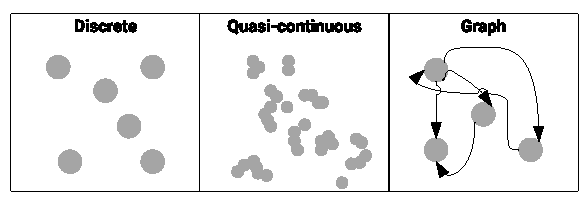
\includegraphics[width=0.8\linewidth]{images/spatialdistribution.pdf}
	\caption{Examples of Discrete, Quasi-continuous and Graph spatial distributions in visualization space, based on various types of spatial reference types. Visual arrangements are present, without loss of generality, in both geographic and abstract spaces.}
	\label{fig:spatialdistribution}
\end{figure}

\begin{defn}\label{dfn:genericpoint_distribution}
	A \emph{Generic Point} induces a \emph{Quasi-Continuous} spatial distribution.
\end{defn}

Generic points are related to entities that can be spatially located in any location within a geographic or abstract grid. Hence, the visual pattern depicted by some of those points induces the notion of smoothness (continuity).

%Figure \ref{fig:continuous} shows a 2D Geographic Heat Map combined with data from citizens' locations while using a route planner mobile application, during their search for nearby stops based on their location. As a citizen can be located anywhere within the city, the visual pattern of data resembles continuity.
%
%\begin{figure*}[hbt]
%	\centering
%	\includegraphics[width=0.6\textwidth]{conceptual/continuous.png}
%	\caption{Example of quasi-continuous spatial distribution in a 2D Geographic Heat Map}
%	\label{fig:continuous}
%\end{figure*}

\begin{defn}\label{dfn:knownpoint_distribution}
	A \emph{Known Point} induces a \emph{Discrete} spatial distribution.
\end{defn}

The requirement of one or more identifier attributes suggests that known points represent entities that have a well-defined location within a region, and are less dense than generic points.

%Figure \ref{fig:discrete} shows a 2D Geographic Heat Map combined with data from realtime schedule requests for bus stops while using a route planner mobile application.
%
%\begin{figure*}[hbt]
%	\centering
%	\includegraphics[width=0.6\textwidth]{conceptual/discrete.png}
%	\caption{Example of discrete spatial distribution in a 2D Geographic Heat Map}
%	\label{fig:discrete}
%\end{figure*}

%\begin{defn}\label{dfn:pointset_distribution}
%A \emph{Point Set} has a \emph{Path} spatial distribution.
%\end{defn}

\begin{defn}
	An \emph{Unordered Point Set} induces a Discrete spatial distribution. Unordered point sets yield structures such as shapes and clusters.
\end{defn}

\begin{defn}
	An \emph{Ordered Point Set} induces a Graph spatial distribution. They form arrangements that resemble the notion of trajectory.
\end{defn}

\begin{defn}
	A \emph{Point Set} inherits the spatial distribution(s) of its points.
\end{defn}

%\begin{defn}
%	A point set inherits the spatial distributions induced by its points. In other words, point sets also induce Discrete and/or Quasi-continuous spatial distributions, according to the types of Points in a set. 
%\end{defn}

The practical purpose of Definition 3.11 is to account for situations in which a visualization provides ways to not only explore point sets as a whole, but to shift the perspective to its intrinsic elements, using interaction mechanisms like semantic zoom. Point sets can be interpreted as paths in the mathematical sense, either ordered or not. Hence, point sets can also induce \emph{Discrete} or \emph{Quasi-Continuous} spatial distributions, depending on the categories of their points.

%sFigure \ref{fig:path} shows an abstract visualization technique that represents the volume of travel intentions between Metro stations in the city of Porto, also using data from a route planer mobile application. Each route plan consists of a point set with two points: origin and destination stations.




%
%\begin{figure}[hbt]
%	\centering
%	\includegraphics[width=0.8\textwidth]{conceptual/path.png}
%	\caption{Example of graph spatial distribution in a chord diagram visualization technique}
%	\label{fig:path}
%\end{figure}
%
%\begin{figure}[hbt]
%	\centering
%	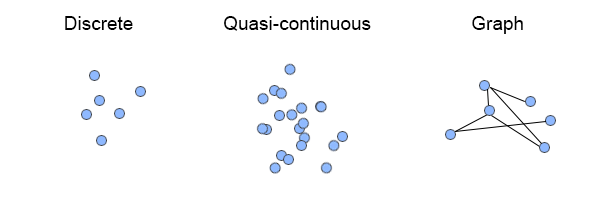
\includegraphics[width=0.85\textwidth]{conceptual/spatialdistribution}
%	\caption{Schematic representation of spatial distributions proposed by the model}
%	\label{fig:spatialdistributions}
%\end{figure}
%

\subsection{Temporal References}\label{sec:temporalreferences}

An entity may have one or more temporal attributes depending on the nature of data. Two types were defined: \emph{Instant} and \emph{Interval}.

\begin{defn}
	An \emph{Instant} is described by a timestamp, i.e. containing date and time, and an optional time zone description.
\end{defn}

\begin{defn}
	An \emph{Interval} is described by two 
	timestamps, corresponding to start and end.
\end{defn}

Although an instant could be considered a zero-length interval in the mathematical sense, we argue that such consideration does not add practical value in the context of data integration and KVTs.

\subsection{Thematic attributes}\label{sec:thematicattributes}

Thematic attributes can have various types, e.g., strings, numerical values, binary file structures or geometric shapes. Due to our orientation towards visualization, we introduce the concept of measures of an entity.

\begin{defn}
	A \emph{Measure} is a certain quantity or degree of something, expressed by a quantitative, ordinal or categorical value.
\end{defn}

In practice, a spatial event instance depicting an accident may have measures as characteristics, such as the number of injured people and damaged vehicles.

%An entity can have more than one measure. We now formalize an intuitive concept of measure, which is inherent to every entity described in the model.
%
%\begin{defn}
%A \emph{Unitary Measure} corresponds to a numeric measure of "1" that is intrinsic to every entity.
%\end{defn}
%
%In practical terms, this measure provides an existential indicator of an entity in a dataset. Such measure intuitively appears when performing simple actions like counting the number of entities in a dataset. For instance, the unitary measure is used in the car accidents dataset to count the total number of accidents during a given period.

\subsection{Transformations}\label{sec:analyzer}

Domain experts carry analytical tasks by performing data transformations (e.g. queries) or more complex operations (e.g. data mining techniques) to extract useful information. We define a \emph{transformation} as a sequence of operations that uses raw data as input, and produces a new dataset as output. This output may contain the same entities found in raw data, and new ones that derive from such operations.

%From a cognitive standpoint, we assume that a transformation can be seen as the formalization of an analytical task, which in turn yields questions about data. In this article, transformations are assumed to be queries. Figure \ref{fig:cognitivetransformation} illustrates such assumption.

%\begin{figure}[ht]
%	\centering
%	\includegraphics[width=0.85\textwidth]{conceptual/conceptualtransformation}
%	\caption[Representation of transformations as the formalization analytical tasks]{Representation of transformations as the formalization of analytical tasks in terms of queries}
%	\label{fig:cognitivetransformation}
%\end{figure}

The output of a transformation, herein defined as a set of \emph{output variables}, may contain spatio-temporal references, depending on the output they generate. Likewise, it can generate new measures based on raw data, or use existing ones as output. The existence of spatial references in the output of a transformation implies that there are also visual spatial patterns associated with it. 
The following proposition demonstrates this statement.

\begin{proposition}
A \textit{transformation} may have zero or more spatial distributions.
\end{proposition}
\begin{proof}
	 Let $T$ be a transformation that yields $\{o_1,...,o_n\}$ as output variables, where $O_s \subseteq O$ is a non-empty subset of $O$ containing spatial references, with $1 \leq i \leq n$. By definition, a spatial reference $a_i$ induces one or more spatial distributions, hence the output of $T$ also induces one or more spatial distributions. In the null case, it suffices to consider that all outputs are attributes other than spatial references.
\end{proof}

%For example, consider a sample dataset showing ticket validations for bus and metro routes in Porto, Portugal, in Figure \ref{fig:example_analyzer}. A simple transformation example is given, which groups the number of ticket validations by fare zones. The count of validations is a new measure built upon existing measures in raw data.
%
%In this example, the transformation is given by the simple SQL query:

%	\begin{lstlisting}
%SELECT Zona, COUNT(*) as CountOfValidations
%FROM table
%GROUP BY Zona
%	\end{lstlisting}
%
%Where $O=\{\texttt{Zona,CountOfValidations}\}$ and $O_s=\{\texttt{Zona}\}$.


%\begin{sidewaysfigure}
%	\centering
%	\includegraphics[width=\textwidth]{conceptual/example_analyzer.png}
%	\caption{Example of transformation. The number of ticket validations is aggregated into fare zones}
%	\label{fig:example_analyzer}
%\end{sidewaysfigure}

\subsection{Visualization techniques}
\label{sec:vis}

A visualization technique has one or more features and provides one or more interaction tasks. Visualization techniques features are the intrinsic components for data visualization. The proposed model specifies four features: \emph{input variable}, \emph{reference frame}, \emph{spatial dimensionality} and \emph{temporal arrangement}. The last three features are derived from a classification of visualization techniques from \cite{Aigner2011}.

\emph{Input variables} are responsible for receiving the values from output variables (of a transformation) that will be mapped onto visual variables.

\emph{Reference frame} describes the ability of a visualization technique to represent \emph{geographic} (georeferenced) data, i.e. map-based visualizations, and \emph{abstract} data.

\emph{Spatial dimensionality} describes the number of dimensions used by the visualization canvas, e.g. 2D or 3D.

\emph{Temporal arrangement} describes how the time dimension is represented on the visualization canvas, e.g. linear, cyclic.

%As an example, consider the prototypical chord diagram visualization technique in Figure \ref{fig:path}. It requires two input variables for source and destination, and one for weight. The prototype provides four interaction tasks: overview, filter, focus plus context, and dynamic queries. The technique has an abstract reference frame, and a linear temporal arrangement. Such conceptual specification is represented in Figure \ref{fig:chord}.
%
%\begin{figure*}[hbt]
%	\centering
%	\includegraphics[width=\textwidth]{conceptual/visualization}
%	\caption{The conceptual description of a possible implementation of the chord diagram visualization technique}
%	\label{fig:chord}
%\end{figure*}

\subsection{Empirical knowledge}
\label{sec:empiricalknowledge}

Empirical knowledge allows for the specification of the users of a KVT, herein considered domain experts, and the annotation of feedback collected during its use.

A user has an analytical profile, which is specified according to the system's objectives. For instance, in our former work, we approached experts that belonged to strategical and operational profiles \citep{Sobral2017}. Such characterization is not meant to be neither exhaustive nor unique.

We define two perspectives for user feedback. The first consists of statements related only to a visualization technique, such as ratings about one or more usability factors as in \cite{Aigner2011}, e.g. visual complexity, or more subjective statements, e.g. ``this visualization is recommended for analyzing ridership from smart card transactions".

The second perspective allows users to provide specialized feedback about visualizations with respect to a transformation, which is defined as a \emph{cross rating}. In cases in which the feedback is provided as a quantitative measure, a technique rating has a rating score related to a rating component. Qualitative feedback is expressed in terms of categorical values. A quantitative rating component is subject to a scale and polarization, i.e. whether its value impacts positively or negatively in the overall rating. Both perspectives for user feedback can feed recommendation methods to provide suggestions of visualization techniques. Section \ref{sec:practical} introduces practical modeling examples of such kinds.

%Figure \ref{fig:empiricalknowledge} provides a conceptual representation of empirical knowledge of two users about the chord diagram technique shown in Figure \ref{fig:path}. User 1 rated the technique with respect to two components: "Visual Complexity", a \emph{quantitative} rating component, and "Recommended analytical profile", a \emph{qualitative} rating component. For instance, visual complexity is a component with negative polarization, in the sense that higher values will are likely to negatively impact the user experience. User 2 rated the technique with respect to the qualitative component "Recommended theme".
%
%\begin{figure}[hbt]
%	\centering
%	\includegraphics[width=\textwidth]{conceptual/empiricalknowledge}
%	\caption[Conceptual representation of empirical knowledge of two users]{Conceptual representation of empirical knowledge of two users about the chord diagram visualization technique. Values in pink and orange depict qualitative and quantitative values, respectively}
%	\label{fig:empiricalknowledge}
%\end{figure}


\begin{figure}[hbt]
	\centering
	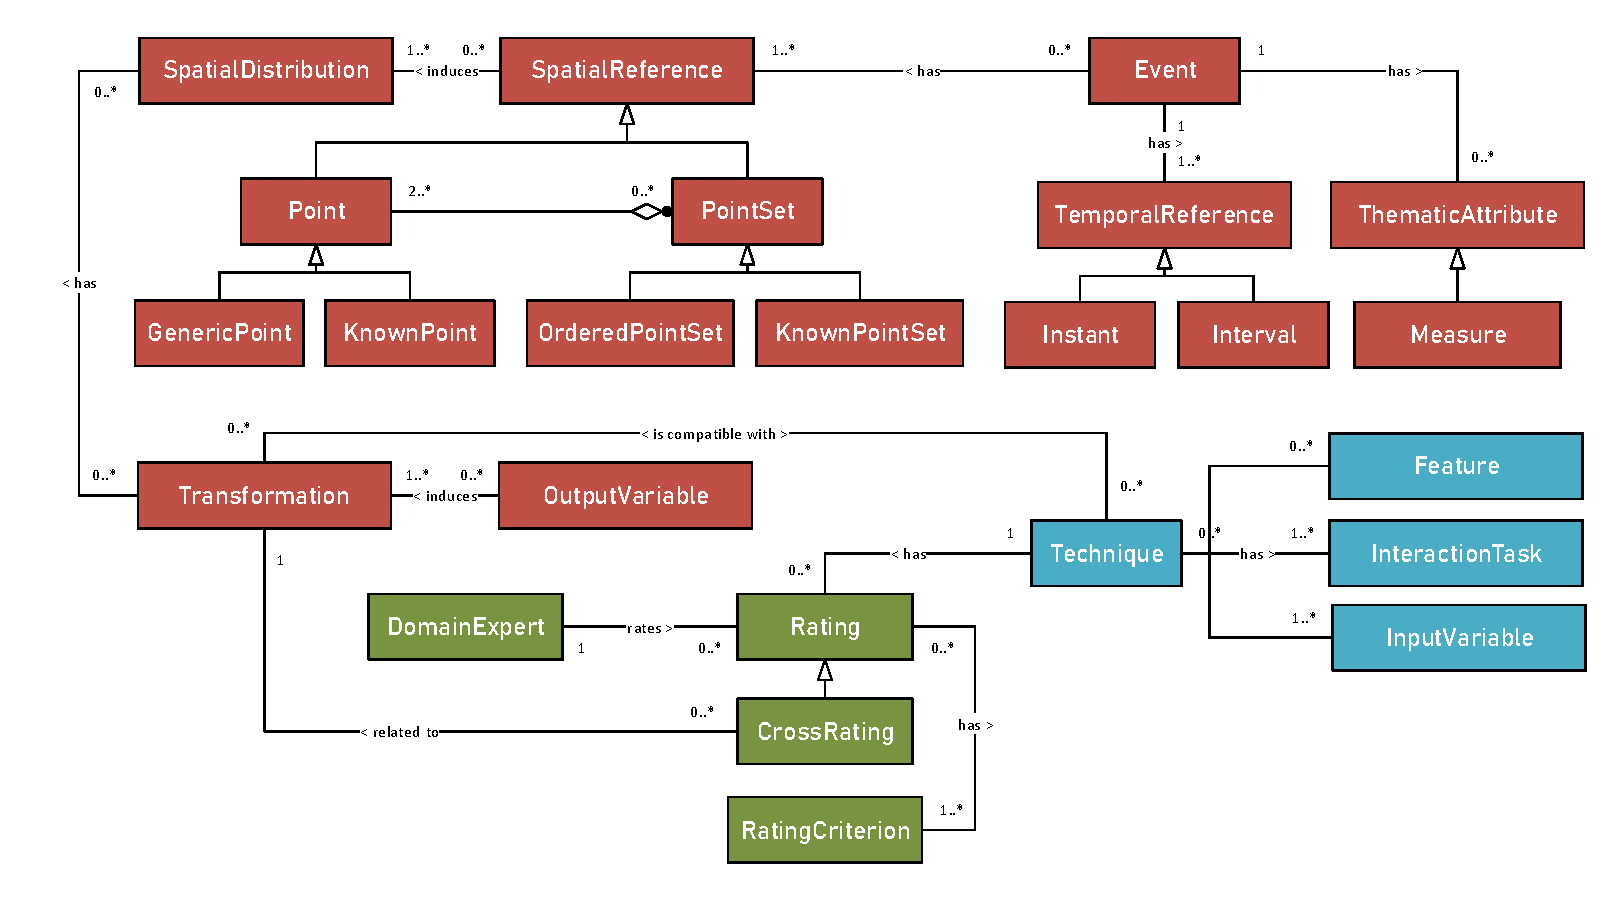
\includegraphics[width=1\textwidth]{images/uml2019}
	\caption[UML Class Diagram for the conceptual model]{UML Class Diagram for the conceptual model, which serves as the basis for the implementation of the VUMO ontology. The three facets represent ITS instance data (gray), visualization technique (blue), and expert knowledge (green).}
	\label{fig:uml}
\end{figure}


\section{The VUMO Ontology}\label{sec:vumo}

%\textcolor{gray}{\textit{This chapter is based on the paper ..., submitted to the International Journal of Transportation Systems}}

%\vspace{5mm}

This section describes the Visualization-oriented Urban Mobility Ontology (VUMO), which lays the semantic foundation for integrating S-T urban mobility data from heterogeneous sources, and building knowledge-assisted visualization tools. VUMO supports the following tasks:

\begin{itemize}
	\item Integration of multi-source heterogeneous urban mobility data related to spatial events, and their description in terms of transportation network elements;
	\item Specification of analytical tasks that domain experts want to carry out in the form of data transformations (queries);
	\item Annotation of visualization techniques implemented in a visualization tool, using concepts from Information Visualization theory;
	\item Annotation of empirical domain expert knowledge, e.g. user information and feedback about visualization techniques in the form of qualitative or quantitative ratings, which can feed recommendation methods;
	\item Rule-based inference of implicit knowledge from instance data that is relevant for the data exploration and visualization process, e.g. implicit links between instances from distinct datasets; characteristics of data transformations; and compatibility between data transformations and visualization techniques.
\end{itemize}

The structure of VUMO is modular, i.e. classes and properties were thought with the goal of having a well defined role on the development of KVTs, according to the following pipelines we defined:

\begin{enumerate}
	\item \emph{Data integration}: visualization tools should allow to integrate data from multiple sources. The data structure not only maintains the original attributes of instance data; the structure is also used to infer visual attributes that can be considered when recommending visualization techniques;
	\item \emph{Visualization technique design and development}: a visualization technique should be characterized in terms of its intrinsic attributes. Such attributes are considered during rule-based inference of compatibility between visualization techniques and data transformations (defined in Subsection \ref{sec:analyzer}), and to aid users on the process of finding appropriate visualization techniques;
	\item \emph{Visualization technique evaluation and specification of users}: user feedback about visualization techniques should be formalized by using the constructs available in the ontology. The annotation of users (domain experts) can also be exploited by recommendation methods.
\end{enumerate}

%VUMO does not constrain the technological stack for the development of visualization techniques, hence they can be developed from scratch or with frameworks such as D3.js or Processing. However, it is naturally assumed that instance data should be expressed in RDF triples.

VUMO is an OWL ontology that conforms to the OWL 2 RL profile, which is a syntactic subset of OWL 2 that supports rule-based inference by trading some of its logical expressiveness \citep{owl}. The implementation of inference rules and functions uses the SPIN vocabulary and modeling language, hence they are expressed as queries in standard SPARQL language, which are \emph{de facto} technologic standards for the Semantic Web. The ontology was built according to a top-down approach, i.e. upper classes and properties were defined and further refined, and reuses existing ontologies for topological spatial relationships (GeoSPARQL) and organization of abstract knowledge (Simple Knowledge Ontology Specification). Given that VUMO is strongly oriented to practical contexts, concepts were modeled after analyzing real-world datasets. In addition, the ontology implements a full semantic counterpart of the Google Transit Feed Specification (GTFS) schema, to facilitate the integration of data published according to this standard.

Subsection \ref{sec:upperclasses} introduces the upper classes of VUMO. Subsections \ref{sec:umc}, \ref{sec:dc}, \ref{sec:vc} and \ref{sec:duc} thoroughly describe the ontology upper classes and their components. Section \ref{sec:vumorules} describes the rules and functions embedded into VUMO that support inference of implicit knowledge.
%Section \ref{sec:vumoreuse} specifies which existing ontologies were reused.
% Subsection \ref{sec:vumosimplecase} describes how VUMO can support user-oriented methodologies for visualization techniques development, according to the aforementioned pipelines.



%\begin{table*}[htbp]
%%\renewcommand{\arraystretch}{1.3}
%\caption{Main features of the VUMO ontology}
%\label{tbl:vumofeatures}
%\begin{tabular}{c|l|l|l}
%    \hline
%      &  Description & Count & Examples\\
%    \hline
%    \hline
%
%    \multirow{5}{*}{\textit{Metrics}}   &   Entities & 100 & Classes, properties and individuals  \\
%	& Classes & X & \texttt{BusStop} \\
%	& Object properties & X & \texttt{hasSpatialDistribution} \\
%	& Data properties & X & \texttt{hasDuration} \\
%	& Individuals & X & \texttt{Strategical} \\
%
%	\hline
%
%    \multirow{3}{*}{\textit{Axioms}}   &   Total of Axioms & 100 & \texttt{:BusStop rdf:type rdfs:Class}  \\
%	& Domain axioms & X & \texttt{BusStop} \\
%	& Range axioms & X & \texttt{hasSpatialDistribution} \\
%
%    \hline
%
%    \multirow{3}{*}{\textit{Annotation}}   &   URI & \multicolumn{2}{l}{\texttt{http://purl.org/vumo\#}}  \\
%    & Namespace & \multicolumn{2}{l}{\texttt{vumo}}   \\
%    & OWL Profile & \multicolumn{2}{l}{OWL RL} \\
%    \hline
%    \hline
%\end{tabular}
%\end{table*}


%The process of ontology development considered the definition of competency questions, i.e. requirements in the form of structured questions that the ontology should answer. An example of competency question is "How is a transportation journey characterized?" \citep{Kathia2013}. In the context of VUMO, we defined the following competency questions:
%
%\begin{enumerate}
%	\item How to characterize an urban mobility event that occurs in a transportation network?
%	\item How to characterize the visual features of an event?
%	\item How to characterize a visualization technique?
%	\item How to characterize a user of a visualization system?
%	\item How to represent the analytical domain tasks of a system user in terms of data transformations?
%	\item How to represent empirical knowledge from system users?
%\end{enumerate}




%}

\subsection{Upper classes}
\label{sec:upperclasses}
% antigo
%The re-use of existing ontologies is a desirable practice, as it enhances interoperability of existing semantic data. The following ontologies are used by VUMO:

%\begin{itemize}
%\item Basic Geo Vocabulary (\textit{geo}): represents information about "latitude, longitude and spatially-located things, using WGS84 as a reference datum";
%\item Semantic Sensor Networks (\textit{ssn}): represents information about sensors, their properties and readings;
%\item General Transit Feed Specification (\textit{gtfs}): describes structural information of PTSs, e.g. stops, routes, schedule and fares.
%\end{itemize}

%VUMO provides a set of rules to (1) infer implicit information in data, (2) derive visualization-related features from data and transformations, based on the conceptual model defined in Section \ref{sec:conceptualmodel}, and (3) to infer compatibility of a visualization with one or more transformations.

%Inference rules are expressed as SPARQL queries with the SPARQL Inference Notation (SPIN) vocabulary.  SPIN also provides an API built on top of Apache Jena, a framework for developing ontology-based applications with inference support. Subsection \ref{subsec:rules} describes VUMO rules.

%Inference rules are expressed with the SPARQL Inference Notation (SPIN) vocabulary. SPIN is a vocabulary that provides an API built on top of Apache Jena, a framework for developing ontology-based applications. Subsection \ref{subsec:rules} describes VUMO rules. Subsection \ref{subsec:rules} describes VUMO rules.

%By design, it is proposed that recommendation algorithms evaluate two criteria: \textit{compatibility} and \textit{appropriateness}. Compatibility ensures that it is possible to visually encode the output of a transformation. Appropriateness enriches the quality of recommendations by processing expert knowledge.% VRSs are expected to implement recommendation algorithms to measure the latter criterion.

VUMO is divided into four upper classes:

\begin{itemize}
	\item \emph{UrbanMobilityConcept (UMC)}: a superclass for all classes that describe urban mobility concepts, including spatial events;
	\item \emph{DataConcept (DC)}: a superclass for all classes that relate to S-T data and data transformations, as in Subsections \ref{sec:spatialreferences}-\ref{sec:analyzer};
	\item \emph{VisualizationConcept (VC)}: a superclass for all classes that characterize a visualization technique, its features and interaction tasks, as in Subsection \ref{sec:vis};
	\item \emph{DomainExpertConcept (DEC)}: a superclass for all classes that characterize domain experts and their empirical knowledge about visualization techniques, as in Subsection \ref{sec:empiricalknowledge}.
\end{itemize}

Table \ref{tbl:vumoroles} shows the role of classes in each pipeline. A main role ($\star$) means that visualization tools developers (and users) will mostly use elements from that class on a specific pipeline. An auxiliary role ($\circ$) means that such a class is mostly referred indirectly (automatically) through rule-based inference, thus not requiring human intervention, unless it is desired to extend the ontology capabilities, e.g. by introducing new rules.
% In the following sections, examples will demonstrate the role of each class across all pipelines.

\begin{small}
	\begin{table}[htb]
		\centering
		\caption{The role of each superclass on the pipelines of a visualization system. A main role ($\star$) indicate a strong, direct use of elements of that class on a pipeline. An auxiliary role ($\circ$) indicate that such class mostly support a specific pipeline, through rule-based inference, thus requiring minimal to none manual intervention.}
		\label{tbl:vumoroles}
		\begin{tabular}{lcccc}
			\toprule
			Pipeline & UMC & DC & VC & DUC \\ \midrule
			Data integration & $\star$ & $\circ$ &  &  \\
			Visualization design and development & $\circ$ & $\circ$ & $\star$ & $\circ$ \\
			Visualization evaluation and system user specification & $\circ$ & $\star$ & $\star$ & $\star$ \\ \bottomrule
		\end{tabular}
	\end{table}
\end{small}




Upper classes branch out into subclasses that represent more specific concepts. VUMO contains Object and Datatype properties to relate instances from the aforementioned classes. Semantic data is herein represented using the standard form, i.e. subject-predicate-object triples, according to the Resource Description Framework (RDF) data model. Table \ref{tab:vumoconcepts} provides a natural language definition for each first-level subclass.

%Throughout the text, classes, properties and instances are written in monospaced font, e.g. \texttt{ns:semanticThing}, where the prefix \texttt{ns} indicates a namespace, i.e. the ontology in which the property is defined. For instance, \texttt{geo} is the prefix of the Basic Geo vocabulary, which is used to describe spatial coordinates \citep{geo}. No prefix was used to refer to VUMO components. 


%\newpage
%\afterpage{
%\begin{landscape}
\setcounter{table}{1}
\begin{sidewaystable}
	%\begin{tiny}
	%\begin{table*}[htbp]
	%\renewcommand{\arraystretch}{1.3}
	\caption{Upper classes of VUMO and their respective first-level subclasses}
	\label{tab:vumoconcepts}
	\centering
	\begin{tabular}{c|l|p{14cm}}
		\toprule
		Upper class  &  Subclass & Definition\\
		\midrule
		
		\multirow{5}{*}{\textit{\shortstack{Urban\\ Mobility\\ Concept \\(UMC)}}}   &   \textit{Agent} & - An entity that is part of the urban mobility network, which can perform actions such as \textit{Event}s.\\
		& \textit{InfrastructureComponent} & - A physical or abstract entity. \textit{Agent}s can use it (in)directly trigger \textit{Event}s, or to provide them with context information.\\
		& \textit{Event} & - An action performed by one or more \textit{Agent}s, which may take place in multiple space and time dimensions.\\
		\hline
		
		\multirow{5}{*}{\textit{\shortstack{Data\\Concept\\(DC)}}}    &   \textit{SpatialReference}	&	- A type of spatial reference.\\
		&	\textit{TemporalReference}	& - A type of temporal reference. \\
		&	\textit{SpatialDistribution}	& - A type of visual arrangement of spatial data. \\
		&	\textit{SpatialDistributionAxiom} & - An abstract container for the spatial distribution axioms defined in the conceptual model. \\
		&	\textit{Transformation} & - A sequence of operations (e.g. query) that yields new information from raw data.  \\
		
		\hline
		\multirow{3}{*}{\textit{\shortstack{Visualization\\Concept\\(VC)}}}	&	\textit{Technique}	& - A visualization technique available in a VUMO-based visualization system. \\
		&	\textit{Feature}	& - An intrinsic characteristic of a \textit{VTechnique}. \\
		&	\textit{InteractionTask}	& - An interaction task available in a \textit{Technique}. \\
		
		\hline
		
		\multirow{11}{*}{\textit{\shortstack{Domain\\Expert\\Concept\\(DEC)}}}		&	\textit{DomainUser}	& - A user of a VUMO-based visualization system. \\
		&	\textit{DomainUserProfile}	& - The profile of a \textit{DomainExpert} with respect to the context of his/her activities, e.g. \textit{Strategical}, \textit{Operational}. \\
		&	\textit{Rating}	& - An abstract container that stores rating information made by a \textit{DomainUser} with respect to a \textit{Technique}. \\
		&	\textit{RatingComponent}		& - An abstract component evaluated in a rating that impacts the user experience, e.g. \textit{Difficulty}, \textit{Visual clutter}. Such components are divided into \textit{Positive/NegativeRatingComponent}. \\
		&	\textit{CrossRating}	& - An abstract container that stores rating information about a \textit{Technique} with respect to a \textit{Transformation}. A \textit{CrossRating} provides a specialized rating by relating a \textit{Technique} to a \textit{Transformation}. \\
		
		
		\bottomrule
	\end{tabular}
	%\end{table}
	%\end{tiny}
	%\end{landscape}
\end{sidewaystable}
%}

%To facilitate understanding, we provide illustrative examples related to the context of Porto, Portugal. The namespace \texttt{porto} is used whenever we refer to instance data related to the city's public transportation system data. Depending on the complexity of the example, we also introduce a visual representation of the corresponding triples for the sake of readability.
%\subsection{UrbanMobilityConcept (UMC)}
%\label{sec:umc}

\subsection{UrbanMobilityConcept (UMC)}
\label{sec:umc}

UMC concepts are fundamental to semantic integration of raw ITS data. The \texttt{Agent} and \texttt{InfrastructureComponent} subclasses group structural concepts of a transportation system. An \texttt{Event} enables to describe distinct types of spatial events, e.g. smart card transactions from AFC systems, trajectories from AVL sensors, among others. Table \ref{tab:umc} provides a natural language definition for the subclasses of UMC.

%\newpage
%\afterpage{
%\begin{landscape}
\setcounter{table}{1}
\begin{sidewaystable}
	%\begin{table}[htb]
	%\renewcommand{\arraystretch}{1.3}
	\caption{First-level and further subclasses of UrbanMobilityConcept (UMC)}
	\label{tab:umc}
	\centering
	\begin{tabular}{c|l|p{12cm}}
		\toprule
		Subclass  &  Second-level subclass & Definition and further subclasses (if applicable)\\
		\midrule
		
		\multirow{3}{*}{\textit{Agent}}   &   \textit{Operator} & - A transportation operator, e.g. bus or subway companies, taxi agencies and shared bicycles operators).\\
		& \textit{Passenger} & - An individual who uses a public transportation system. \\
		& \textit{Vehicle} & - An action performed by one or more \textit{Agent}s, which may take place in multiple space and time dimensions, e.g. buses, trains and bicycles.\\
		\hline
		
		\multirow{7}{*}{\textit{\shortstack{Infrastructure\\Component}}}    &  \textit{Line}	& - A PTS line that may consist of various \textit{Route}s.\\
		&	\textit{Node} &	- A node of the transportation network graph, e.g. \textit{BusStop}, \textit{SubwayStation}, \textit{Sensor}, \textit{BicycleStation}.\\
		&	\textit{Zone}	& - A pre-defined geographic zone used for a specific purpose, e.g. to define fares. \\
		&	\textit{Route} & - A path followed by a \textit{Line}. Lines may consist of several routes\\
		&	\textit{RouteSegment} & - An elementary part of a \textit{Route}, generally defined by two \textit{Node}s. \\
		&	\textit{Ticket}	& - A ticket that allows a passenger to travel within a public transportation network. \\
		&	\textit{TicketType} & - The type of a ticket.  \\
		
		\hline
		\multirow{8}{*}{\textit{Event}}	&	\textit{TravelEvent}	& - A travel made by a passenger within a transportation network triggered by an action, e.g. \textit{TicketValidation}, \textit{BicycleTrip}.\\
		&	\textit{TravelIntention}	& - An intention of traveling within a transportation network, based on information requests, e.g. schedule requests or route plans. \\
		&	\textit{SensorReading}		& - A reading made by a \textit{Sensor}. \\
		&	\textit{SocialMediaPost}	& - A post from social media regarding transportation information. \\
		&	\textit{TripEvent}	&	- A trip made by a \textit{Vehicle}, e.g. bus or taxi. \\
		&	\textit{UnexpectedEvent}	& - An unforeseen \textit{Event}, often capable of (partly) disrupting a transportation network in some way. \\
		
		\bottomrule
	\end{tabular}
	%\end{table}
	%\end{landscape}
	%}
\end{sidewaystable}

%The example below describes two instances: one \texttt{Operator} and one \texttt{Vehicle}, along with some properties.
%
%
%In VUMO, the property \texttt{ownedBy} is defined as the inverse equivalent of \texttt{owns}. Hence, the triple \texttt{porto:STCP :owns porto:Bus3801} could be automatically inferred. The next example shows the instantiation of a bus stop (a node). 

If applicable, an instance can be provided an identification by asserting the property \texttt{hasID} or its semantically equivalent subproperties, such as \texttt{hasInternalID} or \texttt{hasFriendlyID}. To illustrate the utility of multiple ID properties, consider an example of bus stop shown in Figure \ref{fig:stcp_stop} (left) from the city of Porto. \texttt{AEPT1} is a user friendly identification used by passengers to consult schedules using real time services. From the operator's perspective, two internal identifiers are used: \texttt{STCP\_AEPT1} or \texttt{54}. In the AFC dataset, which does not follow a standard schema, the three IDs uniquely determine the stop within their distinct semantic contexts, yet they refer to the same entity. The semantics of the OWL language allows the inference that all given IDs relate to the same entity.

The bus operator (STCP) dataset describes the network according to a different schema: GTFS. The same stop is described in Figure \ref{fig:stcp_stop} (right). After integration, both stop instances are need to be aligned, so that computers can recognize them as semantically equivalent. The \texttt{owl:sameAs} property is used for that purpose. In particular, the latitude and longitude coordinates are slightly different across datasets. The distinct fare zones (N10 and VCD8) are due to the age of datasets, with the GTFS one being the most recent. In Section \ref{sec:practical}, it is discussed how VUMO supported semantic equivalence of fare zones in the context of a recent change in Porto's public transportation network.

\begin{figure}[htbp]
	\centering
	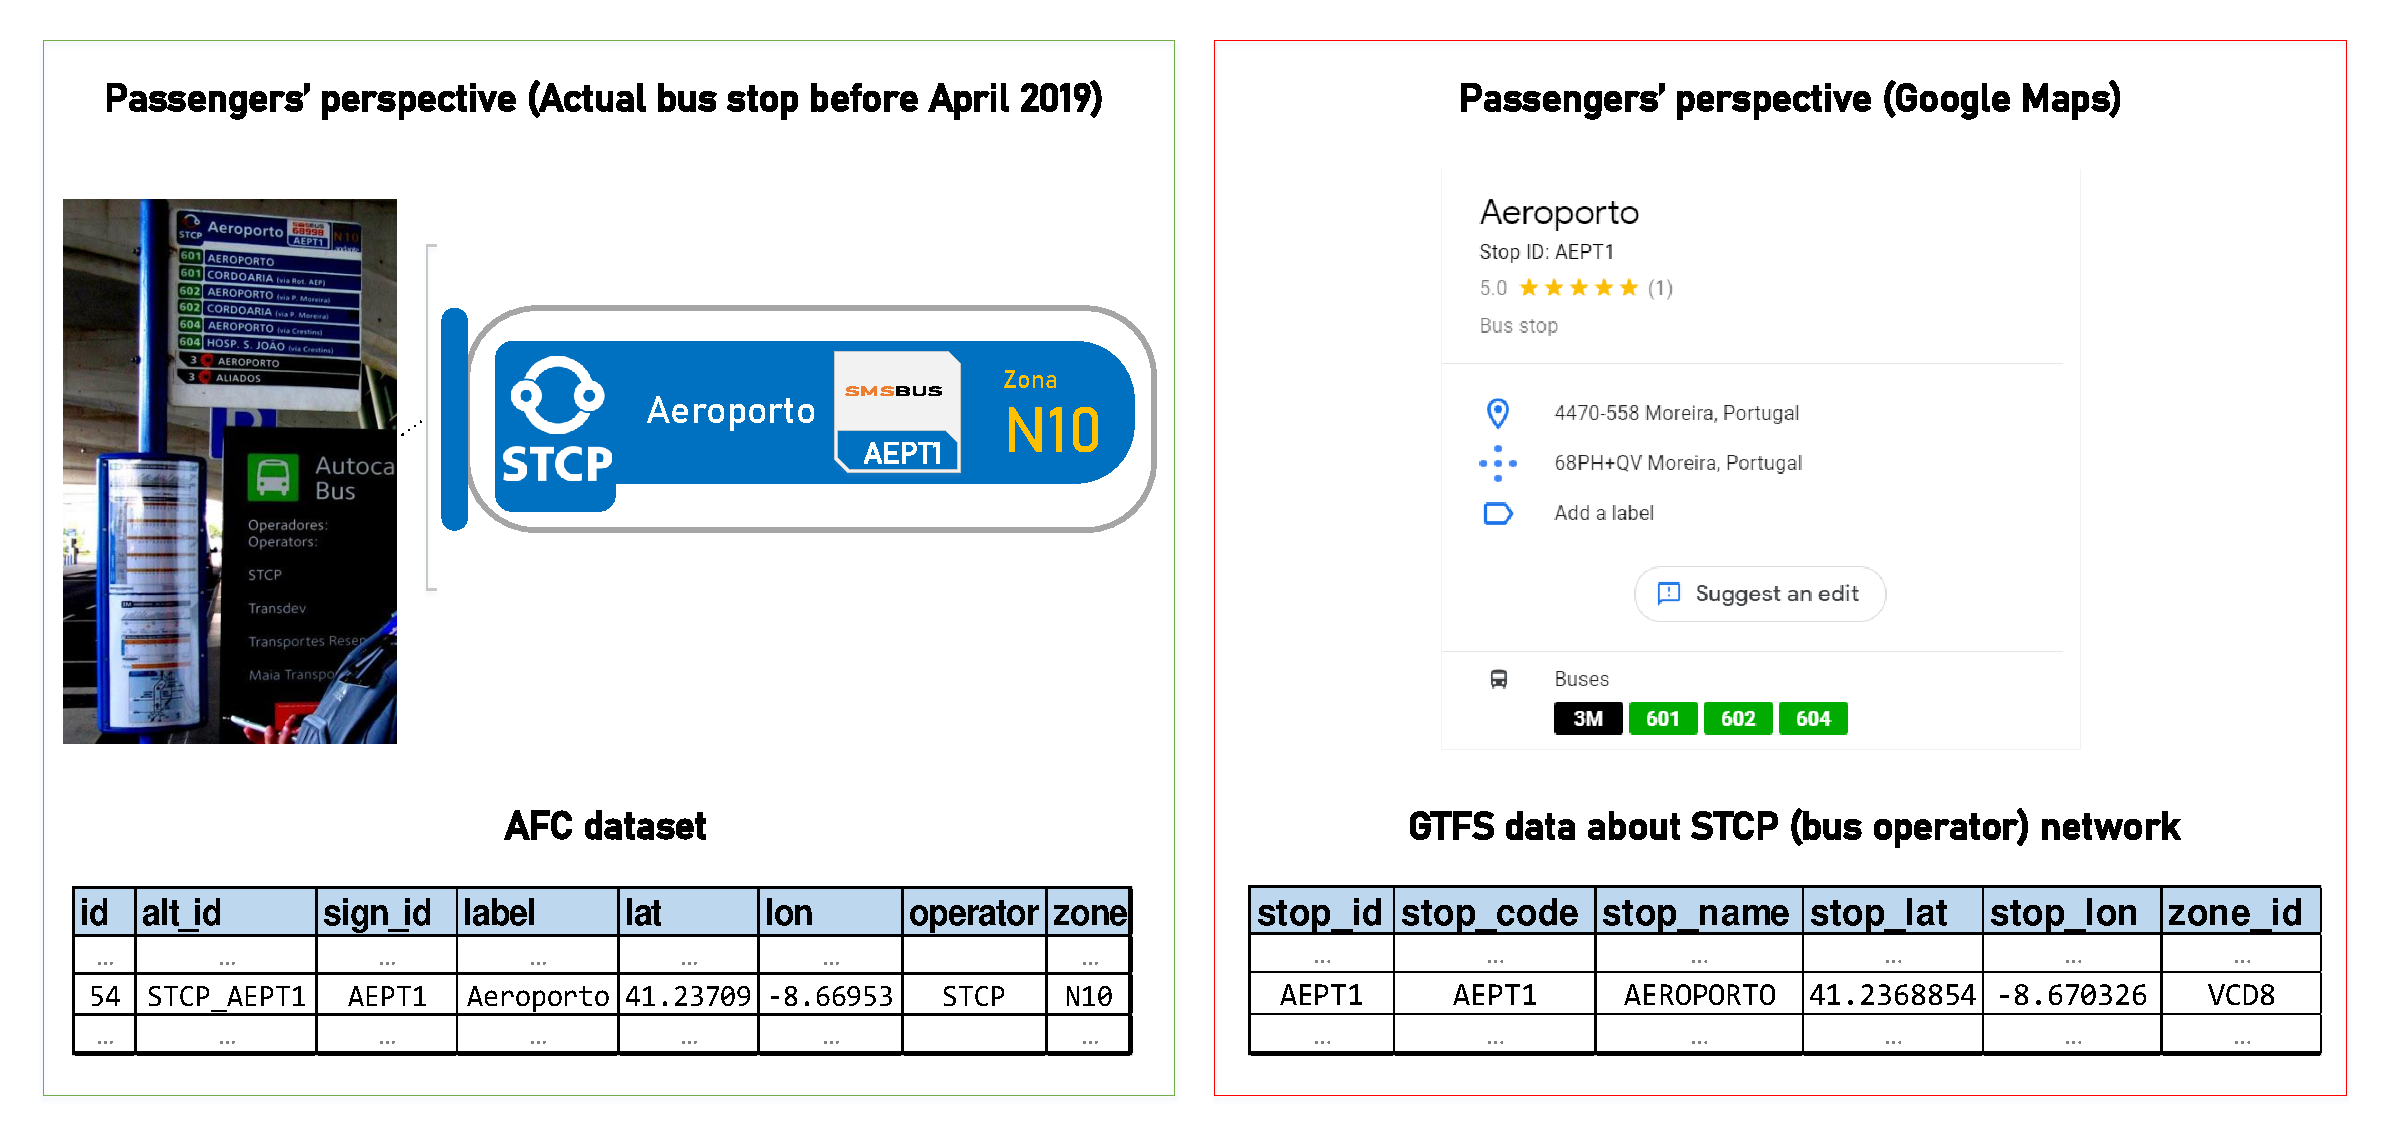
\includegraphics[width=\linewidth]{images/aept_dataset.pdf}
	\caption{An illustration of a bus stop sign of STCP operator in Porto (left), and its representation with the AFC dataset from the smart card operator. The identification AEPT1 is meant to be used by passengers when checking schedules in a real-time service. From the operator's perspective, multiple internal identifications may exist for the same stop. The GTFS representation of the network (right) has a different schema in comparison to the AFC dataset and different values for each attribute, yet they refer to the same bus stop. VUMO's semantics is able to align heterogeneous instance data while preserving their distinctiveness.}
	\label{fig:stcp_stop}
\end{figure}

%
%Figure \ref{fig:aept1} provides a visual representation of the triples that describe the bus stop instance AEPT1. The property \texttt{hasName} is defined as a subproperty of \texttt{rdfs:label} to provide a user-readable version of a resource's name; in this case, \texttt{Aeroporto}. The property \texttt{operates} is an inverse property of \texttt{operatedBy}, thus it is possible to infer the triple

%\begin{figure}[htbp]
%	\centering
%	\includegraphics[width=0.5\linewidth]{vumo_paperbased/portoAEPT1}
%	\caption{Visual representation of the RDF graph that describes the AEPT1 stop}
%	\label{fig:aept1}
%\end{figure}


% \texttt{porto:STCP :serves porto:AEPT1}.
%
%
%The same applies to the properties \texttt{locatedInZone} and \texttt{hasZoneElement}. A zone, for instance, can be described by asserting triples that indicate its boundary points.
%
%
%The instantiation of a line can be described in terms of several routes and their respective route segments, as in the serialization below. Figure \ref{fig:line300} provides a visual representation of the corresponding graph.


%\begin{figure}[htbp]
%	\centering
%	\includegraphics[width=1\linewidth]{vumo_paperbased/line300}
%	\caption{Visual representation of the RDF graph that describes the bus line 300}
%	\label{fig:line300}
%\end{figure}

%A ticket can be instantiated and described in terms of its ticket type, and other properties such as the zone in which it can be used.
%
%
%
%The next three examples show possible modeling approaches for different event types. Firstly, a ticket validation was defined in terms of the trip (instance of \texttt{TripEvent}) in which the validation occurred. An important note is the distinction between the property \texttt{hasDateTime}, which represents instants, and the properties \texttt{hasStartDateTime} and \texttt{hasFinishDateTime}, which are meant to represent intervals.
%
%
%Secondly, the following route plan was defined in terms of its origin and destination locations. Intermediate points (waypoints) can also be represented by using the property \texttt{:hasWaypoint}.
%
%
%Alternatively, the specification may use an interval temporal reference. The property \texttt{hasDuration} can be used to describe the duration of an event. Moreover, it is shown on Section \ref{sec:vumorules} (rule R3) how a VUMO rule can infer the duration of events (a measure) when intervals are specified.
%
%Thirdly, the following description of a car accident was defined in terms of a spatial reference that has no specific identification, i.e. it simply consists of geographical coordinates, and has the form of a blank node.

Measures are available as as subproperties of \texttt{hasMeasure} and expect literal values. Some of the existing properties include:

\begin{itemize}
	\item \texttt{hasDuration};
	\item \texttt{hasNumberOfInjuredPassengers};
	\item \texttt{hasNumberOfAvailableBicycles}.
\end{itemize}

The latter two properties can be used to describe, for example, an \texttt{Accident} or the status of a \texttt{BicycleStation}. It is possible to infer all measures related to a spatial event or entity, as they are subproperties of \texttt{hasMeasure}.

VUMO facilitates the integration of geometry information for spatial references by supporting WKT literals that describe geometric entites like points, polygons and collections of such kinds. The alternative dual representation uses the WGS84 vocabulary to encode latitude and longitude of points. Polygons are represented as linked lists using RDF properties that semantically encode an ordered relation. In practice, most datasets still do not encode geospatial data as WKT elements beforehand. VUMO provides built-in SPIN rules that automatically infer its dual. Figure \ref{fig:umc_spatialtemporalreferences_exemplos}(a) shows an example in which a dataset. In (b), the polygon that describes a fare zone consists of a linked list of points, from which its WKT counterpart was inferred. The dual representation preserves the semantics of geospatial data, even if a RDF triple store does not support GeoSPARQL. The built-in semantics of VUMO allows the inference of spatial references that are not originally asserted in data, due to the transitivity of the property \texttt{location}. For instance, Figure \ref{fig:umc_spatialtemporalreferences_exemplos}(c) demonstrates how a ticket validation instance \texttt{TV1} is automatically inferred to have the zone \texttt{VCD8}, as it contains the bus stop \texttt{AEPT1}.

Temporal references can be expressed in manifold forms depending on the desired type of data granularity, by using the constructs from the Time ontology. For instance, Figure \ref{fig:umc_spatialtemporalreferences_exemplos}(c), the temporal reference is a timestamp. In Figure \ref{fig:umc_spatialtemporalreferences_exemplos}(d), an origin-destination flow measurement \texttt{OD1} has a recurrent temporal reference, \texttt{Weekdays-AM-Peak}, which was created to depict morning peak traffic period between 7 a.m. and 9 a.m.. The representation of temporal references in such a fashion allows for a finer and reusable representation of temporal entities, and facilitates the construction of data queries, which would otherwise be cumbersome to express in relational databases and SQL dialects.

\begin{figure}[htbp]
	\centering
	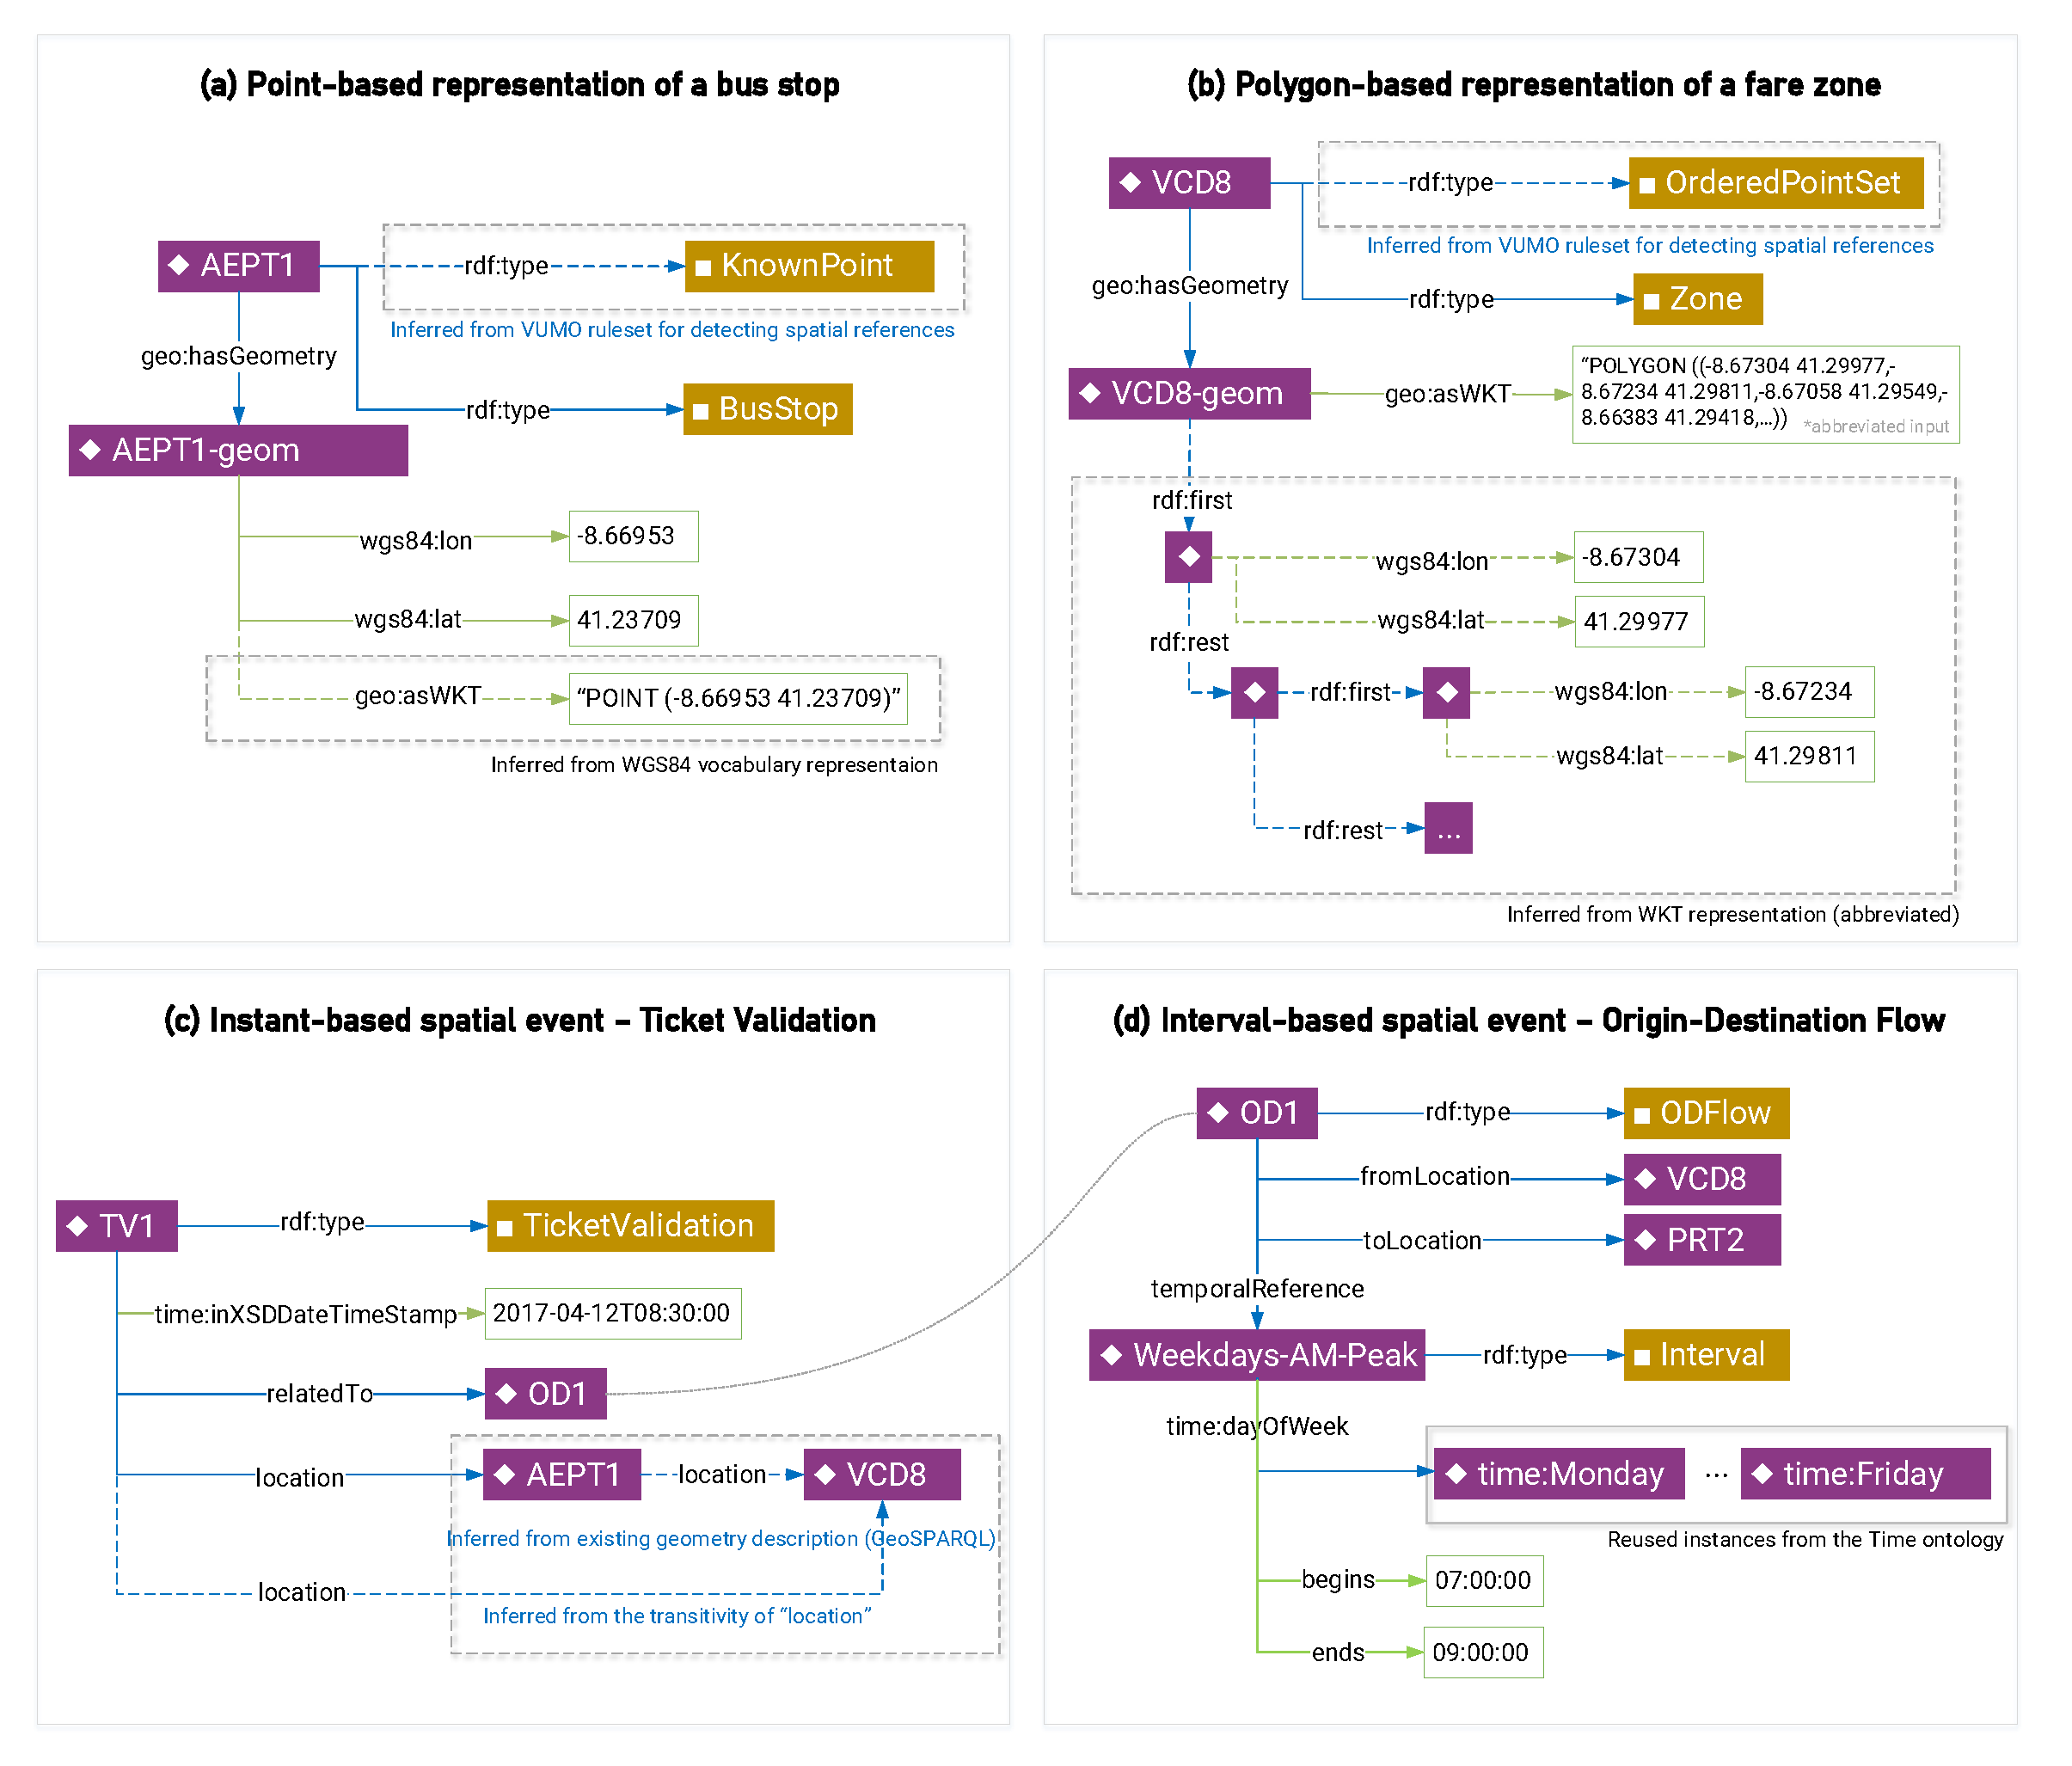
\includegraphics[width=\linewidth]{images/umc_spatialtemporalreferences_exemplos.pdf}
	\caption{Semantic representation of two spatial references and their geometries: a bus stop (left) and a fare zone (right). The AEPT1 instance contains a point-type geometry originally described with the WGS84 vocabulary. The VCD8 instance contains a polygon-type geometry in WKT. VUMO's built-in logic automatically infers the dual representation of each geometry, and the type of spatial reference.}
	\label{fig:umc_spatialtemporalreferences_exemplos}
\end{figure}

As the volume of integrated instance data grows, it is possible to visualize the complex interrelation between datasets. Figure \ref{fig:rdfgraph} shows the interconnection between instance data from various datasets, which is described in Section \ref{sec:practical}. A symbolic notation was adopted for representing data: classes ($\square$) and their instances ($\lozenge$). Object and Datatype properties are represented by blue and green edges. Solid and dashed edges indicate asserted (explicit) and inferred (implicit) triples, respectively.

\begin{sidewaysfigure}
	\centering
	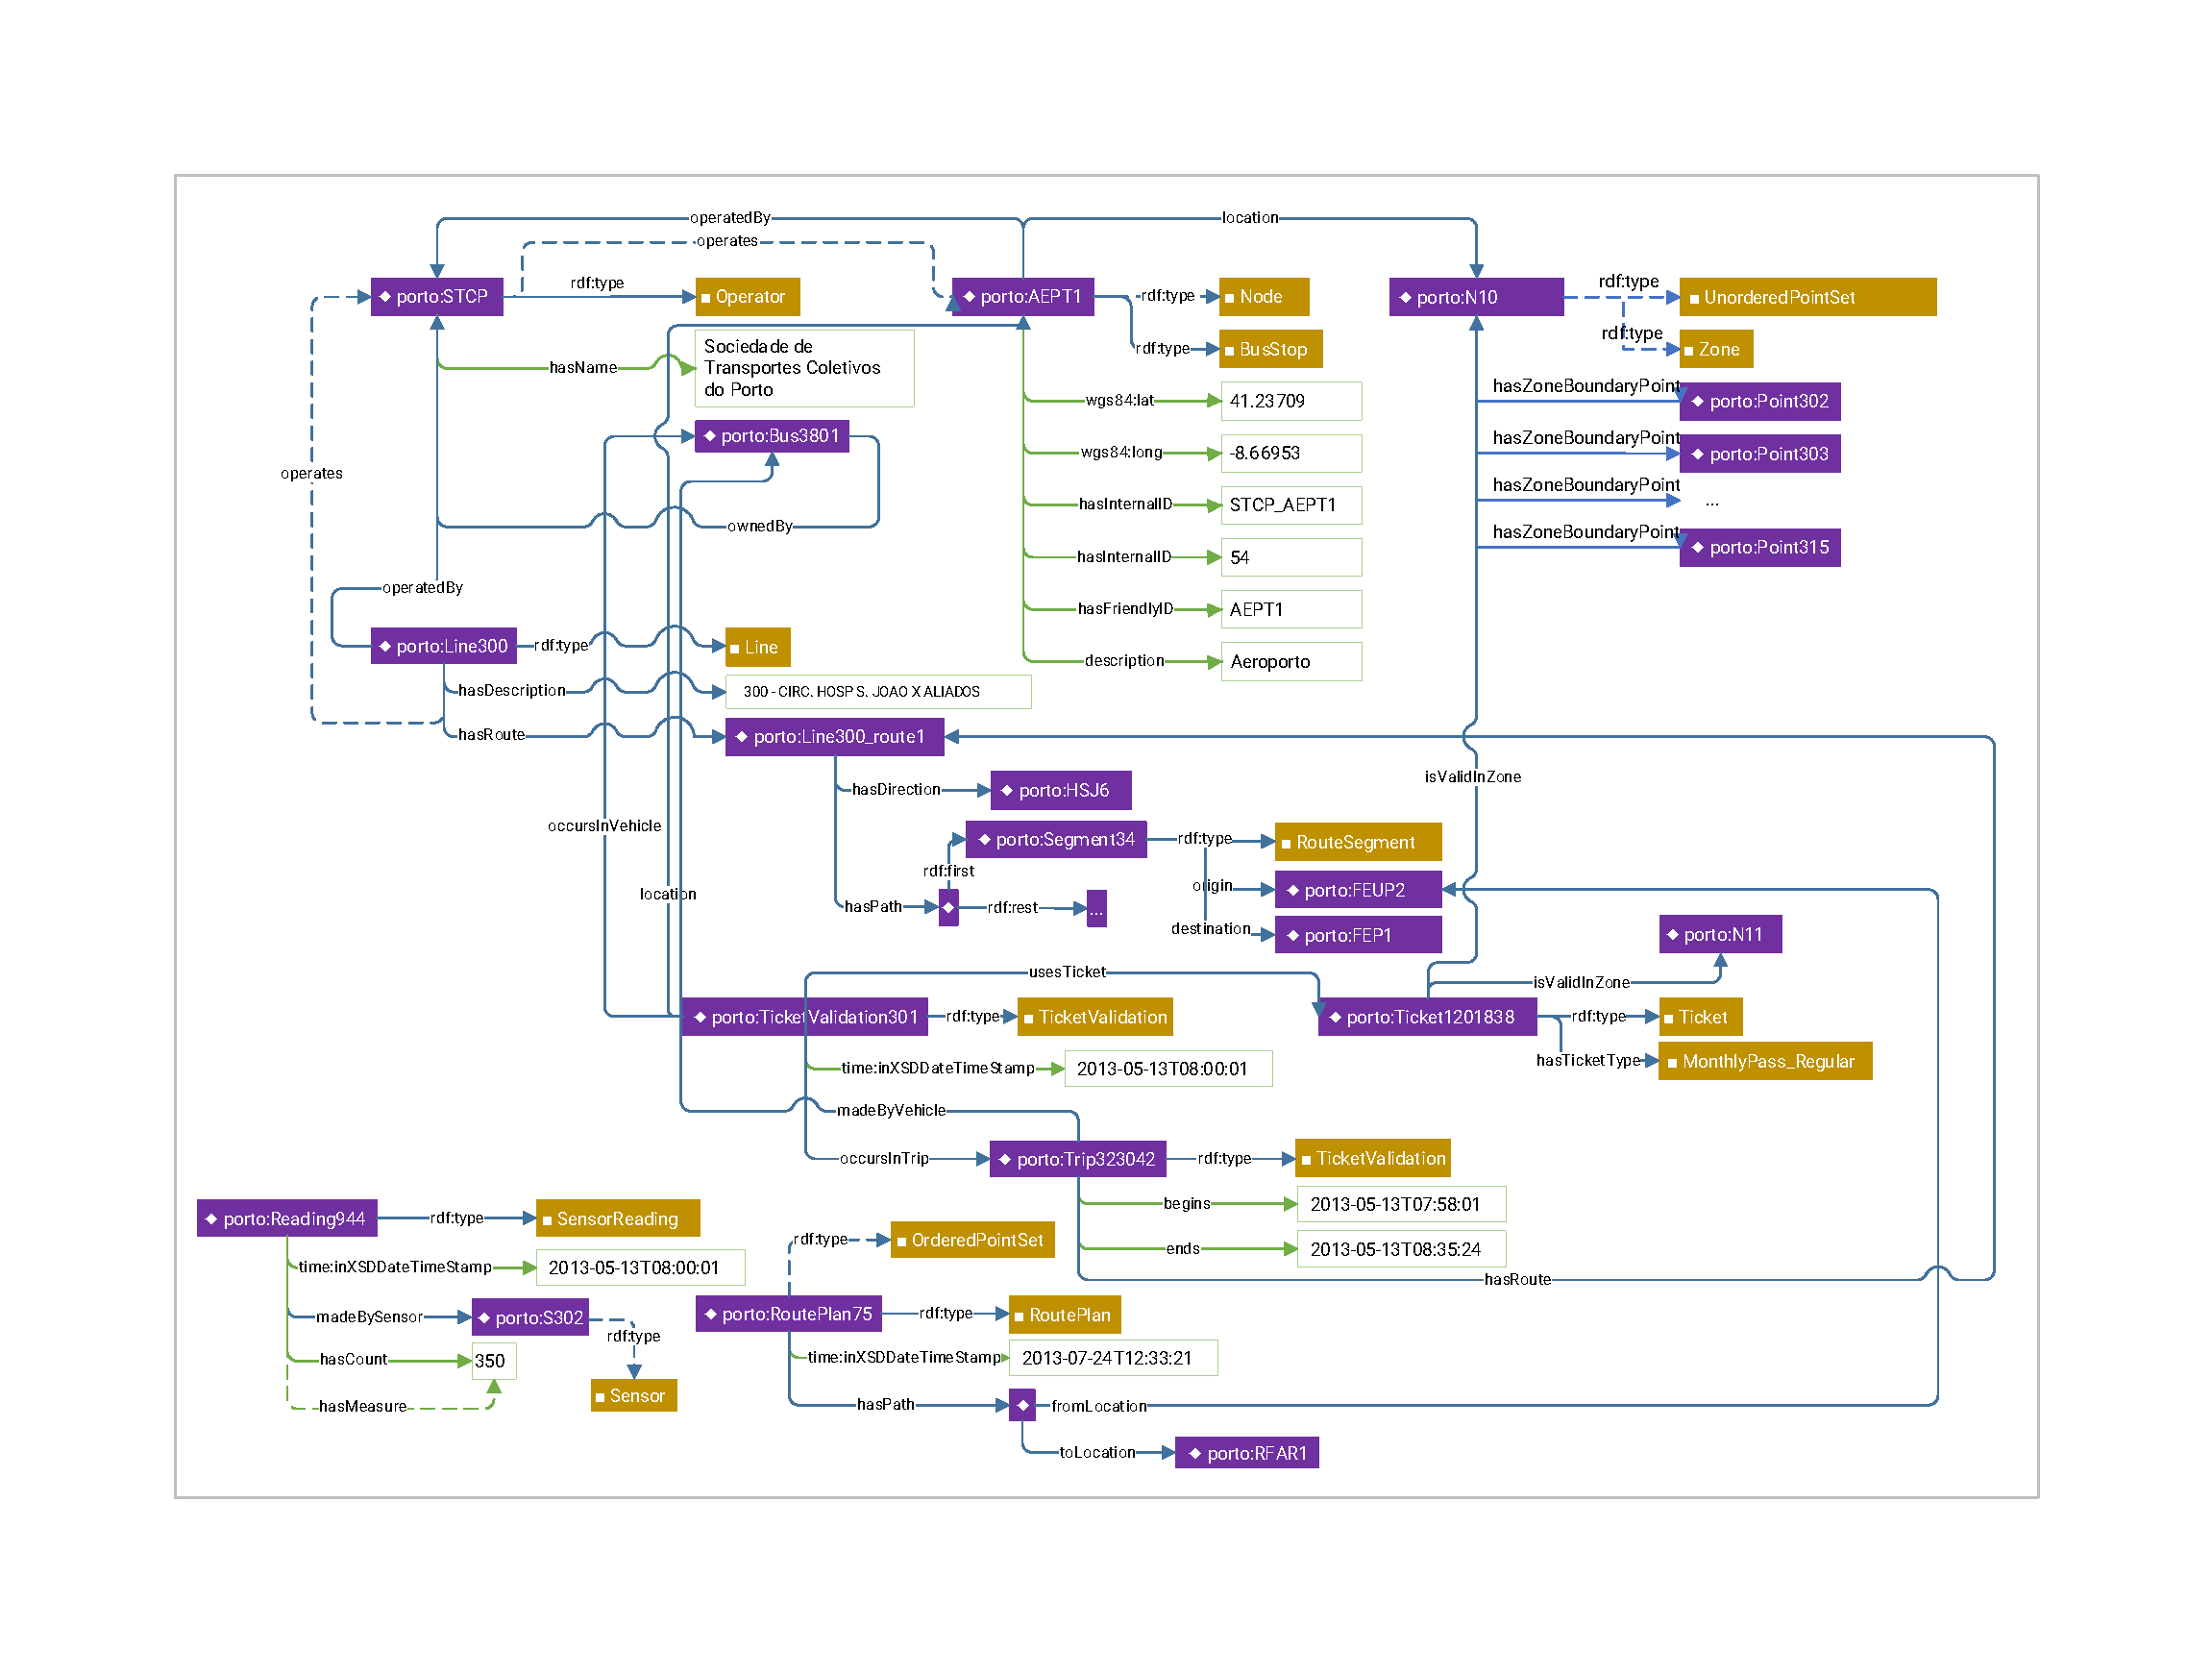
\includegraphics[width=1\linewidth]{images/rdf2}
	\caption{Excerpt of data graph of urban mobility data from Porto, Portugal to be described in Section \ref{sec:practical}, which makes use of several constructs of UMC, and other ontologies such as GeoSPARQL, WGS84, and Time.}
	\label{fig:rdfgraph}
\end{sidewaysfigure}








\subsection{DataConcept (DC)}
\label{sec:dc}

The elements of DC describe structural properties of S-T data and transformations. The subclass \texttt{SpatialReference} is refined into two subclasses:

\begin{itemize}
 \item \texttt{Point}, with further subclasses \texttt{GenericPoint} and \texttt{KnownPoint};
 \item \texttt{PointSet}, with further subclasses \texttt{UnorderedPointSet} and \texttt{OrderedPointSet}.
\end{itemize}

 \texttt{TemporalReference} contains two subclasses: \texttt{Instant} and \texttt{Interval}. The \texttt{Spatial\-Dis\-trib\-ution} class contains three instances: \texttt{Discrete}, \texttt{Quasi-continuous} and \texttt{Graph}.

With the exception of \texttt{Transformation}, the remaining classes defined in DC are not expected to be manipulated directly, as the VUMO rules are responsible for inferring data properties from instance data, i.e. data described in terms of UMC subclasses.

%For instance, a reasoner can infer that the spatial references exemplified in UMC (Subsection \ref{sec:umc}) are a \texttt{KnownPoint}, \texttt{UnorderedPointSet}, \texttt{OrderedPointSet} and \texttt{GenericPoint} respectively, in accordance to the definitions established in Section \ref{sec:modelling}. Hence, the graph of instance data would be semantically enriched with the triples below.

%To instantiate a \textit{Point}, the properties \textit{geo:lat} and \textit{geo:long} are used. If applicable, an identification can be defined with \textit{hasID} or its semantically equivalent subproperties available in VUMO, such as \textit{hasInternalID} or \textit{hasFriendlyID}. To illustrate the utility of multiple ID properties, consider the bus stop shown in Fig. \ref{fig:stcp_stop} from the city of Porto. \textit{AEPT1} is a user friendly identification used by passengers to consult schedules using real time services. From the operator's perspective, one or more identifications can be used, such as \textit{STCP\_AEPT1} or \textit{54}. All IDs uniquely determine the stop within their distinct semantic contexts.


%If a \texttt{PointSet} is subject to a relation of order, properties such as \texttt{hasOrigin} and \textit{hasDestination} are available, as they are subproperties of \textit{hasOrderedSpatialReference}. Otherwise, properties that are not subject to a relation of order should be used, such as \textit{hasZoneBoundaryPoint} or \textit{hasPoint}, which are equivalent subproperties of \textit{hasUnorderedSpatialReference}.

%The description of the subclasses of the \texttt{TemporalReferenceType} class is given in Section \ref{sec:vumoreuse}, in which we discuss the reuse of existing ontologies.

%The definitions of spatial distributions (see Section \ref{subsec:spatialdistributions}) are represented as instances of \texttt{SpatialDistributionAxiom}. The goal of this subclass is to serve as an abstract container for the definitions about spatial distributions that are internally used by VUMO rules to infer the visual patterns of instance data and data transformations.
%
%In practice, spatial distribution axioms are implemented as RDF statements, hence the standard properties \texttt{rdf:subject}, \texttt{rdf:predicate} and \texttt{rdf:object} are used. Notice that the definition of the spatial distribution axiom for a \texttt{PointSet} applies to both subclasses \texttt{Unordered\-PointSet} and \texttt{OrderedPointSet}.

In VUMO, data transformations are modeled as instances of \texttt{Transformation}, and their queries can be expressed in SPARQL. The SPIN vocabulary translates a plain-text query in to a graph. Such specification is seamless to the user. Moreover, we leverage this capability to infer implicit knowledge from transformations, i.e. spatial distributions, tags (themes), and compatibility with visualization techniques.
%
%Recalling the transformation illustrated in Figure \ref{fig:example_analyzer}, which groups the number of ticket validations by fare zones, a possible modeling approach is given by the following example:

%The SPARQL query is represented in plain-text form using the \texttt{spin:query} property from the SPIN vocabulary. Placeholders \texttt{?start} and \texttt{?finish} receive the values specified by users according to the desired time interval. On a technical note, the class \texttt{Transformation} is a subclass of the \texttt{spin:Template} from the SPIN vocabulary \citep{spin}. This class allows the specification of query templates which are meant to be reused by a system.

%Figure \ref{fig:spinquery} illustrates the graph structure that corresponds to this transformation, which is automatically inferred by the SPIN vocabulary. We found appropriate to represent it in a visual way to facilitate visualization, as the graph is not meant to be human-readable. Although it is out of scope to explain how SPIN works, we argue that such example will facilitate the understanding of VUMO rules that extract implicit knowledge from transformations.
%
%The aforementioned query is represented as a blank node, (blank circle). The first two triples indicate the query type (\texttt{SELECT}) and the variable used for grouping the query results (\texttt{?zone}), respectively. Result variables are those that a query will yield as the result of data transformation. The term \emph{result variables} belongs to the SPIN terminology. In this article, the term \emph{output variables} is used to facilitate the comprehension of their relationship with the \emph{input variables} of a visualization technique. The remaining blank nodes represent all conditions expressed inside the \texttt{WHERE} block. The \texttt{FILTER} operator is also expressed internally as a condition.

\subsection{VisualizationConcept (VC)}
\label{sec:vc}

VC allows for the annotation of visualization techniques. The \texttt{Technique} class is used to create instances that represent the visualization techniques implemented in a visualization tool. \texttt{InteractionTask} refers to interactive mechanisms that a technique provides. Some instances are already available in the ontology, e.g. \texttt{SemanticZoom} or \texttt{Filtering}. \texttt{Feature} comprises intrinsic components related to the graphical and data aspects of visualizations. The subclasses of \texttt{Feature} already have a number of pre-defined instances as shown below:

\begin{itemize}
\item \texttt{ReferenceFrame}: \texttt{Abstract}, \texttt{Geographic};
\item \texttt{SpatialDimensionality}: \texttt{2D}, \texttt{3D};
\item \texttt{TemporalArrangement}: \texttt{Linear}, \texttt{Cyclic};
\item \texttt{TemporalRepresentation}: \texttt{Static}, \texttt{Dynamic};
\item \texttt{InputVariable}.
\end{itemize}

%Visualization techniques are seldom immutable representations of data. Interaction tasks provide means of manipulating visualizations, such as zooming or filtering.

Instances for input variables can have any valid Uniform Resource Identifier (URI). In this article, the names \texttt{var1}, \texttt{var2} and \texttt{var3} were used for clarity. The semantics of the property \texttt{hasInputVariable} can automatically infer that such instances belong to the class \texttt{InputVariable}, as VUMO specifies the \texttt{rdfs:range} of this property to \texttt{InputVariable}.

The property \texttt{hasCompatibleValueType} allows the specification of several datatypes that are accepted by an input variable. %We recommend, as good practice, the use of the XSD standard for data types \citep{xmldatatypes}. 
The property \texttt{isRequired} expects a boolean value. It is used to specify whether an input variable is optional or not. This property is also considered by VUMO when evaluating the compatibility of visualization techniques with data transformations.
%
%The bar chart example provides two interaction tasks: dynamic queries and filtering, which can be represented as the following:

\subsection{DomainUserConcept (DUC)}
\label{sec:duc}

DUC allows for the annotation of empirical domain user knowledge. Such knowledge can be used to assess \textit{appropriateness} of visualizations. Users are represented as instances of \texttt{DomainUser}, where each user has one or more \texttt{DomainUserProfile}. VUMO provides two pre-defined instances of user profiles: \texttt{Strategic} or \texttt{Operational}.

%\textit{DomainExpert}s would use a  to carry \textit{AnalyticalTask}s, e.g. "\textit{Ridership and travel intentions to bus stops within a public transportation system zone}". An \textit{AnalyticalTask} consist of one or more \textit{Transformation}s that contain the queries to be executed.

\texttt{TechniqueRating}s are statements made by \texttt{DomainUser}s about a \texttt{Technique}. A \texttt{Techni\-queRating} contain one or more statements regarding \texttt{Rating\-Component}s.

VUMO allows for the annotation of specialized ratings. \texttt{CrossRating}s are used to rate a \texttt{Technique} with respect to a \texttt{Transformation}, according to one or more instances of \texttt{Rating\-Component}s.

% The following specification reflects the illustrative example of Figure \ref{fig:empiricalknowledge}.


\subsection{VUMO rules and functions}
\label{sec:vumorules}

Rules and functions extend the capability of the VUMO ontology on regards to inference of new knowledge beyond the intrinsic semantics of OWL and RDF. We developed a set of rules and functions to automatically infer visualization-related properties from instance data, e.g. types of spatial references and spatial distributions, and to infer implicit knowledge from data transformations and visualization techniques. The proposed rules and functions are not meant to be exhaustive, and can be extended to fit the requirements of KVTs. %The SPIN specification of rules and functions is described in Appendix A.


\subsection{Rules}

%Rules infer implicit knowledge from instance data. Such knowledge facilitates data integration and extracts structural characteristics that are relevant to visualization. Most rules consist of direct implications of the conceptual model (Section \ref{sec:conceptualmodel}).

VUMO contains seven rules, labeled from R1 to R7. They are independent in the sense that the execution of a rule during inference is made independently from the others. In general, inference engines execute rules dynamically as new instance data are ingested into a database.

Rules \textit{R1} and \textit{R2} detect spatial references within instance data and infer their type, i.e. points, point sets, and their subtypes. \textit{R3} infers the duration of intervals if their start and finish times are specified. Rules \textit{R4}, \textit{R5} and \textit{R6} infer characteristics of \textit{Transformation} queries based on their structure, namely: spatial distribution (\textit{R4}), themes (\textit{R5}), use of aggregate functions (\textit{R6}). \textit{R7} infers the compatibility between transformations and visualization techniques.


Tables \ref{tab:vumorules_dataintegration} and \ref{tab:vumorules_transformations} provides the pseudocode representation of rules R1-3 and R4-8, respectively. Inferred triples are represented with a specific notation. For instance, $s \in \mbox{\textit{GenericPoint}}$ is equivalent to "$s$ is an instance of \textit{GenericPoint}"; $t \mbox{\textit{ isCompatibleWith }} v$ denotes a subject-predicate-object triple.

%\textit{R3} derives a new measure - the duration of an interval - based on the start and finish times, if applicable.

\begin{tiny}
\begin{table}[htbp]
%\renewcommand{\arraystretch}{1.3}
\caption{Pseudocode representation of VUMO rules related to data integration}
\label{tab:vumorules_dataintegration}
\centering
\begin{tabular}{p{0.5cm}l}
    \toprule
    Rule & Pseudocode\\
    \midrule

	\multirow{7}{*}{R1} & // R1 infers \textit{Point}s and their subtypes \\
	& $s \leftarrow \text{instance of \textit{rdfs:Resource}}$ // receives an instance of any class  \\
	&  \textbf{if} \textit{containsLatitudeLongitude($s$)} \textbf{then} \\
	& \quad \textbf{if} \textit{containsIdentification($s$)} \textbf{then}\\
	& \quad \quad $s \in \text{\textit{KnownPoint}}$ // infers $s$ as an instance of \textit{KnownPoint} \\
	& \quad \textbf{else} \\
	& \quad \quad $s \in \text{\textit{GenericPoint}}$ // infers $s$ as an instance of \textit{GenericPoint}\\
	\hline
	\multirow{8}{*}{R2} & // R2 infers \textit{PointSet}s and their subtypes \\
	&  $s \leftarrow \text{instance of \textit{rdfs:Resource}}$ // receives an instance of any class  \\
	& $P \leftarrow \bigcup_{s} p$ // Points referred by $s$, if any\\
	&  \textbf{if} $|P| \geq 2$  \textbf{then} // $P$ should have at least two Points \\
	& \quad \textbf{if} \textit{isOrdered($P$)} \textbf{then}\\
	& \quad \quad $P \in \text{\textit{OrderedPointSet}}$ // infers $P$ is an \textit{OrderedPointSet} \\
	& \quad \textbf{else} \\
	& \quad \quad $P \in \text{\textit{UnorderedPointSet}}$ // infers $P$ is an \textit{UnorderedPointSet} \\
	\hline
	\multirow{5}{*}{R3} & // R3 infers the duration of intervals, when applicable\\
	&  $e \leftarrow \text{instance of \textit{Event}}$ \\
	& $p_i,p_f \leftarrow$ // ordered temporal reference properties (initial and final)\\
	&\textbf{if} $(e \quad p_i \quad t_i) \wedge (e \quad p_f \quad t_f)$ \textbf{then} // if triples exist for start and finish times \\
	& \quad $e$ \textit{hasDuration} $(t_f - t_i)$ // inferred triple\\
    \bottomrule
\end{tabular}
\end{table}
\end{tiny}



\textit{R4} analyzes conditional clauses for predicates containing  equivalent subproperties of \textit{hasSpatialReference}. If one or more clauses satisfy that condition, the range of such property is used to retrieve the spatial reference type. The corresponding axiom is then used to retrieve the spatial distribution. %For instance, it follows from \textit{A1} that the query in Fig. X induces a \textit{Discrete} spatial distribution, as the property \textit{occursAtNode} has \textit{KnownPoint} as its range, by definition.

\textit{R5} extracts themes, i.e. tags, that describe the urban mobility concepts related to a \textit{Transformation}. The rule finds condition clauses whose properties' ranges are subclasses of \textit{UrbanMobilityConcept}. Themes provide a natural language description of the contents of a \textit{Transformation}.

\textit{R6} verifies if a \textit{Transformation} returns aggregate data, i.e. if at least one \textit{OutputVariable} contains an aggregate function. Such verification occurs while evaluating compatibility, as a \textit{Technique} may expect disaggregate instance data to perform aggregations externally.


\textit{R7} evaluates the compatibility of a \textit{Transformation} with respect to a \textit{Technique}. Compatibility holds if the aggregate requirements (\textit{R5}) match, and if there exists at least one bijective mapping $m$ such that

%\begin{align}
\begin{align*}
    m \colon & O^{\prime} \subseteq O \rightarrow I \\
    & o_j \longmapsto i_k
\end{align*}

and $\theta(o_j) = \theta(i_k) \ \forall (o_j,i_k)$, where $o_j \in O^{ \prime}$ and $i_k \in I$ are the output and input variables, respectively.

$O$ is the set of all output variables returned by a data transformation. $I$ is the set of all input variables of a visualization technique. $O'$ is a subset of $O$.
The function $\theta$ represents an operator that returns the type of an output or input variable, e.g. string, integer, resource.


%\textit{R7} suggests the analytical profile of a \textit{Transformation} based on the query conditions. In brief, it identifies if how broad/narrow are the concepts described in the query body.

\begin{tiny}
\begin{table}[htbp]
%\renewcommand{\arraystretch}{1.3}
\caption{Pseudocode representation of VUMO rules related to data transformations}
\label{tab:vumorules_transformations}
\centering
\begin{tabular}{p{0.5cm}l}
    \toprule
    Rule & Pseudocode\\
    \midrule

	\multirow{9}{*}{R4} & // R4 infers \textit{SpatialDistribution}s of a \textit{Transformation}\\
	&  $t \leftarrow \text{instance}$, $q_t \leftarrow \text{query within } t$, such that $t \in \text{\textit{Transformation}}$ \\
	& $C \leftarrow \bigcup_{q_t} c$ // condition clauses of $q_t$\\
	&  \textbf{for each} $c \in C$ \textbf{do} \\
	& \quad $p_c \leftarrow \text{\textit{property(}}c\text{\textit{)}}$ // receives the property (predicate) of $c$ \\
	& \quad \textbf{if} $p_c \equiv \text{\textit{hasSpatialReference}}$ \textbf{then} \\
	& \quad \quad $r_{p_c} \leftarrow \text{\textit{range(}}p_c\text{\textit{)}}$ // receives the range of property $p_c$ \\
	& \quad \quad $\sigma_{r_{p_c}} \leftarrow \text{\textit{getSpatialDistribution(}}r_{p_c}\text{\textit{)}}$ \\
	& \quad \quad $t$ \textit{hasSpatialDistribution} $\sigma_{r_{p_c}}$ // inferred triple\\
	\hline
	\multirow{8}{*}{R5} & // R5 infers themes (tags) of a \textit{Transformation}\\
	&  $t \leftarrow \text{instance}$, $q_t \leftarrow \text{query within } t$, such that $t \in \text{\textit{Transformation}}$ \\
	& $C \leftarrow \bigcup_{q_t} c$ // condition clauses in $q_t$\\
	&  \textbf{for each} $c \in C$ \textbf{do} \\
	& \quad $p_c \leftarrow \text{\textit{property(}}c\text{\textit{)}}$ // receives the property (predicate) of $c$ \\
	& \quad \textbf{if} $\text{\textit{range(}}p_c\text{\textit{)}} \equiv \text{\textit{UrbanMobilityConcept}}$ \textbf{then} \\
	& \quad \quad $r_{p_c} \leftarrow \text{\textit{range(}}p_c\text{\textit{)}}$ // receives the range of property $p_c$ \\
	& \quad \quad $t$ \textit{hasTheme} $r_{p_c}$ // inferred triple\\
	\hline
	\multirow{9}{*}{R6} & // R6 infers if the query of a \textit{Transformation} returns aggregate results\\
	&  $t \leftarrow \text{instance}$, $q_t \leftarrow \text{query within } t$, such that $t \in \text{\textit{Transformation}}$ \\
	& $V \leftarrow \bigcup_{q_t} v$ // set of output variables of $q_t$\\
	&  \textbf{for each} $v \in V$ \textbf{do} \\
	& \quad \textbf{if} $\text{\textit{isAggregate(}}v\text{\textit{)}}$ \textbf{then} \\
	& \quad \quad $t$ \textit{returnsAggregateResults} \textit{true} // inferred triple\\
	& \quad \quad \textbf{break} // one occurrence is sufficient \\
	& \quad \textbf{else} \\
	& \quad \quad $t$ \textit{returnsAggregateResults} \textit{false} // inferred triple\\
	\hline
	\multirow{8}{*}{R7} & // R7 infers compatibility of a \textit{Transformation}-\textit{Technique} pair \\
	& $t,v \leftarrow$ instances, such that $t \in \text{\textit{Transformation}}, v \in \text{\textit{Technique}}$ \\
	& $O,I \leftarrow \text{output and input variables sets of $t$, respectively}$\\
	& $\xi \leftarrow \varnothing$ // result set of compatible mappings \\
	& \textbf{if} \textit{meetsAggregateRequirements}($t,v$) \textbf{then} \\
	%& \quad \textbf{if} $\text{\textit{range(}}p_c\text{\textit{)}} \equiv \text{\textit{UrbanMobilityConcept}}$ \textbf{then} \\
	& \quad $\xi \leftarrow \text{\textit{findMapping(}}t,v\text{\textit{)}}$ // stores compatible mappings in $\xi$ \\
	&\quad \textbf{if} $|\xi|\geq 1$ \textbf{then}\\
	&\quad \quad $t$ \textit{isCompatibleWith} $v$ // inferred triple \\
    \bottomrule
\end{tabular}
\end{table}
\end{tiny}


%VUMO provides a set of rules that support data integration and visualization recommendation. Rules were built with the SPIN vocabulary, thus they are specified as SPARQL queries. Ontologies that require rule-based reasoning are classified as OWL-RL ontologies. Focus is given to rules that are relevant for visualization. Reasoning over instance data occurs after data integration.

%The conceptual model defined in Section \ref{sec:conceptualmodel} provides the basis for rules that extract features from data. Rules \textit{R1} and \textit{R2} infer whether an instance is a Point or PointSet, respectively, and to which subclass they belong. As shown in Fig. \ref{subfig:rule_point} and \ref{subfig:rule_pointset},

%The SPIN vocabulary allows the definition of \textit{Transformation} queries as an RDF graph. The following rules consist of meta-queries that infer features from \textit{Transformation}s that are relevant for visualization techniques, based on the content and structure of queries. Two rules were implemented to infer spatial distribution (\textit{\textit{R3}}) and themes (\textit{R4}).

%\textit{R3} infer the spatial distribution(s) of a \textit{Transformation} based on the query conditions, specified within the WHERE clause. Each condition (a triple) is evaluated with respect to its predicate (property). If the property is a subproperty of \textit{hasSpatialReference}, the rule retrieves the range of such property, e.g. a Point. Finally, the rule retrieves the spatial distribution by consulting the respective axiom (A1-A4)

%\begin{figure}[!tbp]
%\centering
%\includegraphics[width=5cm]{vumo_paperbased/rule_spatialdistribution.png}
%\caption{Rule \textit{R3} - Inference of spatial distributions of a \textit{Transformation}}
%\label{fig:rule_spatialdistribution}
%\end{figure}

%\textit{R4} infers the urban mobility concepts related to a \textit{Transformation}. For instance, a query may regard \textit{Event}s such as \textit{TicketValidation}s and \textit{ScheduleRequest}s. Such themes work as tags that can be used by recommendation algorithms. \textit{R4} evaluates whether the conditions contain a predicate that expects an \textit{UrbanMobilityConcept} as a predicate. If it does, the concept is related to the transformation with the \textit{hasTheme} property.

%R5 is an auxiliary rule for inferring whether a query returns aggregated data, i.e. according to an aggregate function, e.g. COUNT(), SUM(). Given that a visualization techniques may be developed to perform data aggregation, such information is important for evaluating compatibility. The rule evaluates whether a query contains an aggregate function, which should be followed by a GROUP BY statement. The \textit{Transformation} receives a new triple using the property \textit{returnsAggregatedData}, which can be \textit{true} or \textit{false}.

%Rule R6 evaluates whether a \textit{Transformation} is compatible with a \textit{Technique}. The first condition verifies if the number of output variables of a \textit{Transformation} is lower than the number of non-optional input variables of a \textit{Technique}. If not, the second condition verifies is there is at least one mapping between variables, i.e. if every \textit{OutputVariable} is mapped onto an \textit{InputVariable} of the same tipe, e.g. numeric. The \textit{Transformation} receives a new triple with predicate \textit{isCompatibleWithTechnique} in case the condition is satisfied.

%\begin{figure}
%\centering
%\subfloat[Rule \textit{R1} -\textit{Point} type inference\label{subfig:rule_point}]{\includegraphics[width=7cm]{vumo_paperbased/rule_point.png}}
%\\
%\subfloat[Rule \textit{R2} - \textit{Pointset} type inference\label{subfig:rule_pointset}]{\includegraphics[width=7cm]{vumo_paperbased/rule_pointset.png}}
%\caption{Rules for inferring \textit{Point}s (a) and \textit{Pointset}s (b)}
%\label{fig:r1r2}
%\end{figure}





\subsection{Functions}

Besides compatibility of evaluation of visualization techniques and data transformations, the evaluation of appropriateness is specific to the implementation of recommendation methods of each KVT. VUMO provides embedded functions to assist methods on retrieving asserted empirical knowledge:

\begin{itemize}
    \item \texttt{getTechniqueRating(t)}: returns all ratings given to a visualization technique \texttt{t};
    \item \texttt{getCrossRating(t,v)}: returns all cross ratings assigned to the a transformation \texttt{t} and a visualization technique \texttt{v};
    \item \texttt{getExpertInfo(e)}: returns asserted knowledged related to domain expert \texttt{e}.
    \item \texttt{getBroaderConcepts(c)}: returns concepts that are broader than \texttt{c}, based on the assertions made with the SKOS vocabulary;
    \item \texttt{getNarrowerConcepts(c)}: returns concepts that are narrower than \texttt{c}, based on the assertions made with the SKOS vocabulary;
\end{itemize}

Functions are also stored as SPARQL queries, and take advantage of the SPIN vocabulary to be executed as such.
%
%VUMO was evaluated for logical consistency using third-party reasoners that run several tests: Pellet, FaCT++ and TopSPIN \citep{spin}. The results indicated no inconsistency errors, e.g. logical contradictions. The OOPS! Pitfall Scanner \citep{oops} was also used to detect issues such as missing annotations, which were corrected. Purposely, some properties do not have information about their domains and ranges, in order to avoid undesired side-effects in terms of axiomatic classifications, as well as to reduce inference time. On regards to practical validity, VUMO was used in practical applications, as will be explained in Chapter \ref{chp:practice}. The ontology was revisited several times to refactor properties, classes and instances names, and their specifications.


%
% \begin{table*}[htbp]
% \begin{tiny}
% \centering
% %\renewcommand{\arraystretch}{1.3}
% \caption{Ontologies reused by VUMO}
% \label{tbl:vumoimported}
% \begin{tabular}{l|l|l}
%     \hline
%     Name & Namespace & URI\\
%     \hline
%     \hline
%
%     \small WGS84 Geo Positioning & \small \texttt{geo} & \small http://www.w3.org/2003/01/geo/wgs84\_pos\# \\
%     \small Time Ontology & \small \texttt{time} & \small https://www.w3.org/TR/owl-time\# \\
%     \small General Transit Feed Specification & \small \texttt{gtfs} & \footnotesize http://vocab.gtfs.org/terms\# \\
%     \small Simple Knowledge Organization System & \small \texttt{skos} & \footnotesize https://www.w3.org/2008/05/skos \\
%     \small Web Ontology Language & \small \texttt{owl2xml} & \footnotesize http://www.w3.org/TR/owl2-syntax/ \\
%     \small Resource Description Framework & \small \texttt{rdf} & \footnotesize http://www.w3.org/1999/02/22-rdf-syntax-ns\# \\
%     \small Resource Description Framework Schema & \small \texttt{rdfs} & \footnotesize http://www.w3.org/2000/01/rdf-schema\# \\
%     \small Extended Markup Language vocabulary & \small \texttt{xml} & \footnotesize http://www.w3.org/XML/1998/namespace \\
%     \small Extensible Markup Language schema & \small \texttt{xsd} & \footnotesize http://www.w3.org/2001/XMLSchema\# \\
%
%     \hline
%     \hline
% \end{tabular}
% \end{tiny}
% \end{table*}

%}

%This section demonstrates VUMO applied to semantic integration of data, annotation of visualizations and expert knowledge. The supporting data is related to the public transportation system of Porto, Portugal, and provide information about (a) smartcard ridership for bus and subway services, description of (b) stops and stations, (c) fare zones, (d) ticket types, and (e) usage data from Move-me schedule consultation service. Move-me is a mobile application that provides real-time information about Porto's public transportation system. Two prototypical visualization techniques were developed to support the demonstration. Expert knowledge was collected through exploratory usability tests with local domain experts, who are involved in strategic and operational decisions for the public transportation system. Two prototypical domain experts were defined based on such knowledge.
%
%\subsection{Semantic integration of data}
%
%Datasets were provided in various formats: CSV (a,b), Excel spreadsheets (c,d), and SQL dumps (e). The mapping of each dataset schema onto the VUMO classes and properties is supported by an \textit{ad hoc} parser which also returns semantic instance data in RDF. The resulting graph was stored in a triple store engine. Fig. \ref{fig:instancedata} illustrates an excerpt of the resulting graph containing elements from original source data.
%
%In particular, dataset (b) is described by the schema shown in Fig. \ref{fig:stcp_stop}, where each row corresponds to a stop. Table \ref{tab:correspondence} shows a possible mapping between the source attributes and VUMO properties.
%
%As the RDF graph is independent of source data and their schemes, it is possible to manipulate data from all datasets simultaneously. For instance, \textit{TicketVal30} and \textit{SchedReq12} have \textit{BusStop54} as a common spatial reference.
%
%It follows from \textit{R1} and \textit{R2} that \textit{BusStop54} and \textit{ZoneN10} are \textit{KnownPoint} and \textit{UnorderedPointSet}, respectively. \textit{TicketVal30} and \textit{ZoneN10} are inferred as instances of \textit{TicketValidation} and \textit{PTSZone}, as they are the domain of properties \textit{hasValidationDateTime} and \textit{hasZoneBoundaryPoint}, respectively. Inferences related to domain and range are native to RDF semantics and do not require the specification of inference rules.
%
%
%\begin{figure*}[!tbp]
%\centering
%\includegraphics[width=\textwidth]{vumo_paperbased/rdf.pdf}
%\caption{Excerpt from RDF graph of mobility data from Porto Public Transportation System}
%\label{fig:instancedata}
%\end{figure*}
%
%\subsection{Visualization Knowledge and Data Transformations}
%
%Map-based and abstract visualization techniques were developed: geographic (\textit{GeoHeatMap}) and calendar (\textit{CalHeatMap}) heat maps, respectively. The former depicts the density of instance data in geographic space. The latter depicts density in a daily arrangement. Each day is assigned to a color according to the number of occurrences.
%
%\textit{GeoHeatMap} requires the following input variables: (a) an event instance; (b,c) spatial (latitude and longitude) and (c) temporal references (instant). Variable (a) receives the entity to be plotted, (b,c) provide the instance coordinates on a map, and (d) is used for temporal filtering. \textit{CalHeatMap} requires the same variables but (b,c). Semantic zoom is available in both techniques. By construction, \textit{CalHeatMap} require aggregate data. \textit{GeoHeatMap} does not. Fig. \ref{fig:vis_user} shows the semantic annotation of both visualization techniques.

%\begin{figure}
%\centering
%\subfloat[Geographic heat map\label{subfig:geoheatmap}]{\includegraphics[width=8.5cm]{vumo_paperbased/geoheatmap}}
%\\
%\subfloat[Calendar heat map\label{subfig:calheatmap}]{\includegraphics[width=8.5cm]{vumo_paperbased/calheatmap}}
%\caption{Prototypical visualization techniques compliant with VUMO}
%\label{fig:visualizations}
%\end{figure}

%Let \textit{porto:T1} and \textit{porto:T2} be two data transformations related to the domain task "Analysis of travel events and intentions". \textit{porto:T1} returns the total of ticket validations, the ID and geographic coordinates of each node during a given time period. \textit{porto:T2} returns the same data, except for the coordinates. Their respective SPARQL query formulation is given by Listing \ref{alg:transformation}. The query searches for a subgraph that matches the triple patterns related to events that occured at a given node. The COUNT() function aggregates the results by node.
%
%Let \textit{AT1} be an instance of \textit{AnalyticalTask} described by "analysis of \textit{TicketValidation}s and \textit{ScheduleRequest}s", and \textit{T1} an instance of \textit{Transformation} that implements the following query with five output variables:
%
%\begin{algorithmic}
%
% \label{alg:transformation1}
%
%  \STATE \textbf{SELECT} \textit{?ev ?lat ?lon ?time} COUNT(\textit{?node}) AS \textit{?total}
%  \STATE \textbf{WHERE \{}
%  \STATE \hspace{5mm} \textit{?ev rdf:type (:TicketValidation OR :ScheduleRequest) .}
%  \STATE \hspace{5mm} \textit{?ev :hasDateTime ?time .}
%  \STATE \hspace{11mm} \textit{occursAtNode ?node .}
%  \STATE \hspace{5mm} \textit{?nodeID geo:lat ?lat .}
%  \STATE \hspace{18mm} \textit{geo:long ?lon .}
%  \STATE \hspace{5mm} \textbf{FILTER (}\textit{?time $\geq$ ?arg1} \&\& \textit{?time $\leq$ ?arg2}\textbf{) \}}
%  \STATE {\textbf{GROUP BY} \textit{?node}}
%\end{algorithmic}
%
%\textit{AT1} is linked to \textit{T1} via the property \textit{hasRelatedTransformation}. An \textit{AnalyticalTask} can be linked to one or more \textit{Transformation}s. Arguments \textit{arg1} and \textit{arg2} are placeholder values that can be changed by the user.
%
%From R3 and axiom A1, it follows that \textit{T1} contains a \textit{Discrete} spatial distribution, as the property \textit{occursAtNode} has \textit{Node} as its range, which is defined as semantically equivalent to a \textit{KnownPoint}. R4 yields the tags \textit{TicketValidation} and \textit{ScheduleRequest}. It follows from R5 that \textit{T1} returns aggregate results due to the COUNT function.
%
%It follows from R6 that \textit{T1} is compatible with \textit{CalHeatMap}, but not \textit{GeoHeatMap}, due to the aggregate results requirement. Consider another instance of \textit{Transformation}, \textit{T2}, that implements the same query as \textit{T1} except for the aggregate function. Hence, \textit{T2} is compatible with \textit{GeoHeatMap}, but not \textit{CalHeatMap}.
%
%\begin{figure*}[htbp]
%\centering
%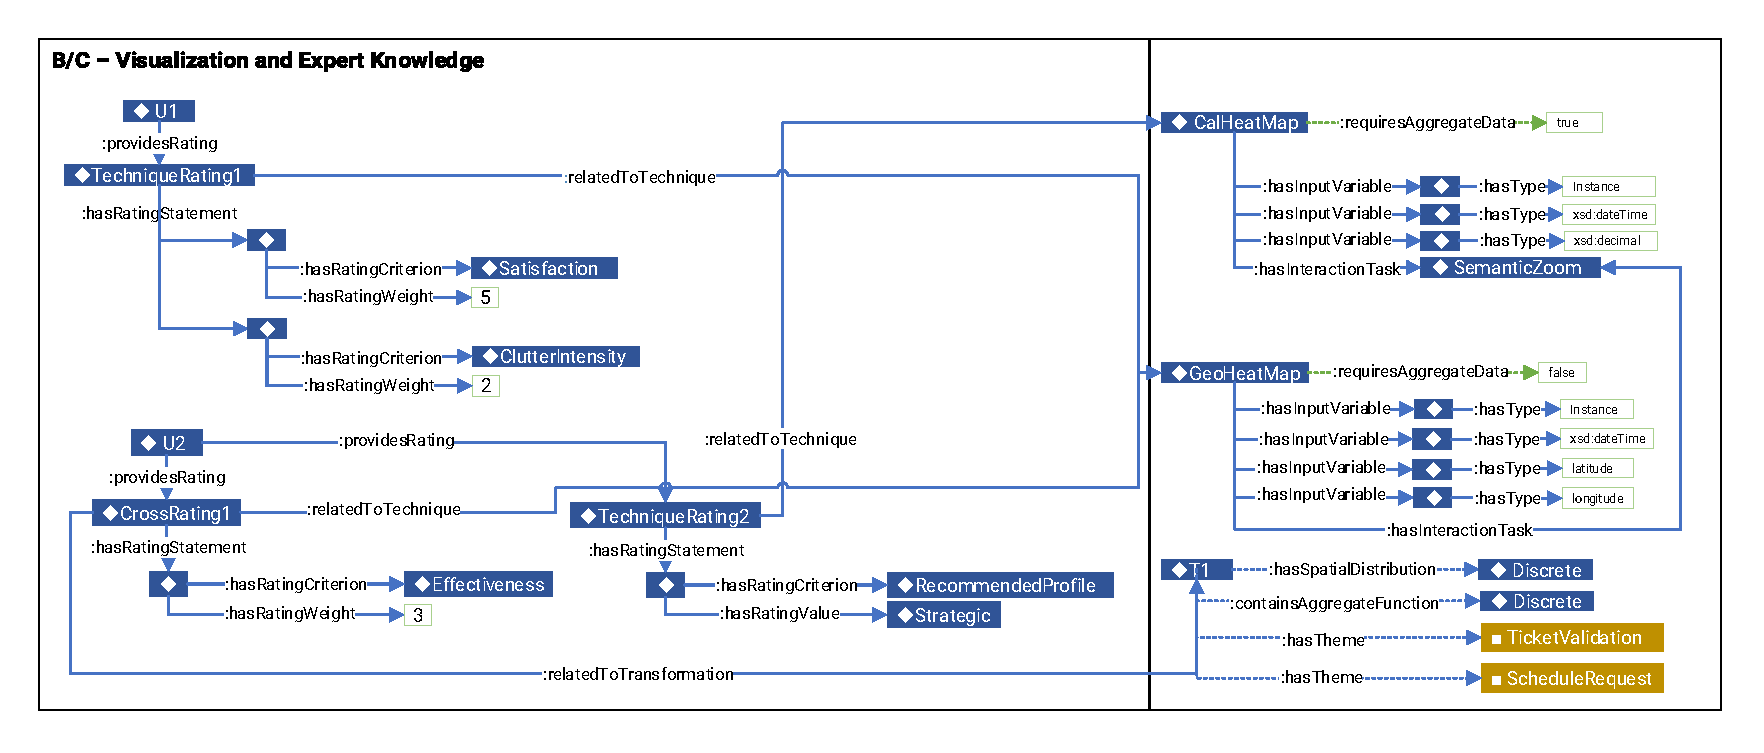
\includegraphics[width=\textwidth]{vumo_paperbased/vis_user.pdf}
%\caption{Excerpt from RDF graph containing visualization and domain experts' knowledge}
%\label{fig:vis_user}
%\end{figure*}
%
%\subsection{Expert Knowledge and Appropriateness Evaluation}
%
%Let \textit{U1} and \textit{U2} be instances of \textit{DomainExpert}, which represent two users of a visualization system, with strategic and operational profiles, respectively. \textit{Strategic} and \textit{Operational} are instances of \textit{DomainUserProfile}. Each user can rate a visualization technique with respect to multiple criteria represented by instances of \textit{RatingCriterion}. Each criterion can be evaluated according to categorical or numerical values. Ratings are stored as instances of \textit{TechniqueRating}. Users can also provide a specialized rating that relates a visualization technique to a data transformation. Such rating is modeled as an instance of \textit{CrossRating}. Fig. \ref{fig:vis_user} exemplifies a general and specialized rating by \textit{U1} and \textit{U2}, respectively.
%
%\textit{U1} stated that the \textit{GeoHeatMap} is appropriate for data transformations that induce a continuous domain. Quantitative ratings were also provided: \textit{Satisfaction} was rated "5" on an arbitrary scale of 0 to 5, and \textit{ClutterIntensity} was rated "2" on the same scale. The latter components are instances of \textit{Positive-} and \textit{NegativeRatingCriteria}, respectively. The type of each component can be used by a recommendation algorithm to define the appropriateness of each visualization technique.
%
%\textit{U2} provided a specialized rating to the same technique and transformation \textit{T1}, and rated "3" on regards to the \textit{Effectiveness} criterion. The same user provided a global rating for \textit{GeoHeatMap}, in which it was stated that the technique is appropriate for users with a \textit{Strategic} profile.
%
%
%\subsection{Asserting new knowledge}
%
%VUMO can be used to formalize new knowledge derived from the use of visualization techniques. In particular, the \textit{CalHeatmap} technique allowed the identification of an abnormal amount of schedule requests for Trindade, the main subway station in Porto. The number of requests is related to the public transportation strike that occurred on June 27th, 2013. The \textit{CalHeatMap} prototype was used to relate all schedule requrest instances on that date to a new event asserted as \textit{Strike27Jun13}, which is an instance of \textit{UnexpectedEvent}. Fig. \ref{fig:strike} shows the resulting graph.
%
%\begin{figure}[htbp]
%\centering
%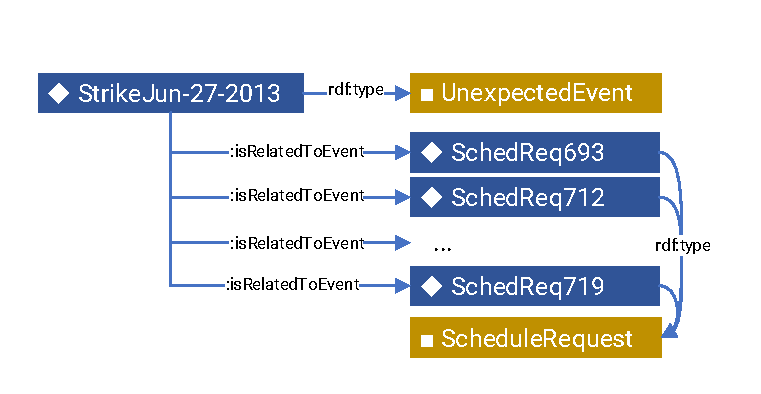
\includegraphics[width=9.3cm]{vumo_paperbased/strike.pdf}
%\caption{An instance of \textit{UnexpectedEvent} represents a public transportation system strike, which is related to several \textit{ScheduleRequest}s}
%\label{fig:strike}
%\end{figure}
%

%\section{Discussion of Results}
%\label{sec:discussion}
%
%For semantic integration of mobility data, the mapping of a dataset schema to VUMO classes and properties should be planned in advance. \textit{Ad hoc} parsers are considered an effective approach to convert raw data onto RDF graphs. A dataset may not be entirely described in terms of VUMO components due to the absence of specific classes or properties. To address that limitation, developers can extend or import additional ontologies which declare additional concepts.
%
%The ontology does not require VRSs to be implemented in a specific programming language. To use VUMO, the only technological requirements are the support to RDF data, OWL ontologies and SPIN inference. Visualization techniques implemented in a VRS should be able to digest RDF data and comply to their annotation, especially on regards to the specification of input variables and interaction features.
%
%VRSs may be impaired by cold start, i.e. absence or lack of sufficient domain expert knowledge to perform recommendations during early system use. VUMO addresses this limitation by evaluating compatibility (\textit{R5}), which can guarantee a minimal set of visualizations for experts to start with.
%
%On regards to transformations, VUMO rules are limited to infer characteristics from queries, as the SPIN vocabulary allows them to be stored as a RDF graph. Still, transformations may assume other specialized forms, e.g. data mining algorithms or simulations. VUMO can still be useful to provide semantic annotation, as developers may manually specify such characteristics.

%The demonstration was performed on a computer with the following configuratrions: I7 32GB of ram. Datasets (a) and e), which contain events data, occupied approximately 1.4 gigabytes. The semantic representation of data as an RDF graph increased to approximately 8 gigabytes, yielding approximately 140 million triples. Despite the size, query operations on an RDF graph tend to keep good performance.

%VUMO can be extended with additional concepts to account for specific needs of various mobility contexts. For instance, new types of events or infrastructure components can be included.

%The SPIN vocabulary provides constructs for building complex rules as SPARQL queries that could not be accomplished using other rule languages such as Semantic Web Rule Language (SWRL).

%VRS may be impaired by cold start, i.e. absence of domain expert knowledge to perform recommendations at start time. Compatibility evaluation (R5) guarantees a minimal set of visualizations, from which experts can start providing recommendations.

%estender a ontologia
%tempo de execucao e tamanho dos arquivos resultantes. em que configuracao?
%todas as propriedades tem domain e range?
%pq SPIN e nao SWRL? *talvez nao seja necessario; dizer apenas sobre SPIN*
%(talvez: inputs para recomendacao)
%num contexto de implementacao, qual e a ordem de inclusao dos dados?

%A system may have not many ratings, and may suffer from cold start. Compatibility guarantees a minimal set of visualizations.

%\begin{table*}[htbp]
%\label{tab:artifacts}
%%\renewcommand{\arraystretch}{1.3}
%\caption{Summary of artifacts that are subject to semantic annotation, according to each phase of a UCD methodology and the three pipelines for the deveopment of semantically-rich, knowledge-assisted visualization systems}
%\label{tab:artifacts}
%\centering
%\begin{footnotesize}
%\begin{tabular}{p{4cm}|l|l}
%    \toprule
%    Pipeline &  Phase & Artifacts for semantic annotation\\
%    \midrule
%    1. Data integration & Transversal to all phases & Integrated urban mobility data\\
%\hline
%     & Problem domain analysis & Analytical profile\\
%    2. Visualization technique  & & Domain users \\
%    design and development & & Data transformations \\
%    & Conceptual development and prototyping & Visualization techniques\\
%		\hline
%    3. Visualization evaluation and specification of system users & Interaction and usability studies & Rating and cross ratings\\
%    \bottomrule
%\end{tabular}
%\end{footnotesize}
%\end{table*}


% This section provides a critical analysis of the VUMO ontology in terms of completeness and scalability. We discuss the proposed formalization of spatiotemporal data, visualization techniques and empirical domain user knowledge, in terms of the corresponding implementations of these concepts in the VUMO ontology.

% An entity is allowed to have multiple spatial and temporal references. Spatial references are asserted as subproperties of \texttt{hasSpatialReference}. Temporal references are asserted as subproperties of \texttt{hasTemporalResourceReference}, if the reference is a resource, or \texttt{hasTempor\-alReference}, if the reference is a literal, e.g. date and time. New subproperties can be instantiated to c, as long as they belong to one of the aforementioned superproperties.

% Points and point sets allow modeling a variety of point-based spatial references found in datasets, which are often specified as one or more geographical coordinates. The built-in rules provide the required logic for inferring the type of spatial reference to instance data, assuming that there is a correct mapping between source data attributes and the properties in the ontology. The proposed implementation makes use of the WGS84 datum, as it is coordinate reference system often found in most datasets.

% The temporal



%
%We presented an illustrative application in which two prototypical visualization techniques were developed and annotated with VUMO. The annotation is expected to be performed by those in charge of the visualization tool development. Finally, we showed how VUMO can support assertion of new knowledge after visual exploration of data.


%\section{A Conceptual Model for a KVT}
%\label{sec:conceptualmodel}
%
%A formalization of spatial urban mobility events is proposed to represent spatiotemporal dimensions and thematic attributes, and to relate those structures to data visualization attributes. The schematic representation of a spatial event is shown in Fig. \ref{fig:uml} as a UML class diagram. Subsections A-D define classes and their interrelations. Subsection \ref{subsec:datatransformations} defines data transformations and their visual attributes.
%
%\begin{figure}[htbp]
%	\centering
%	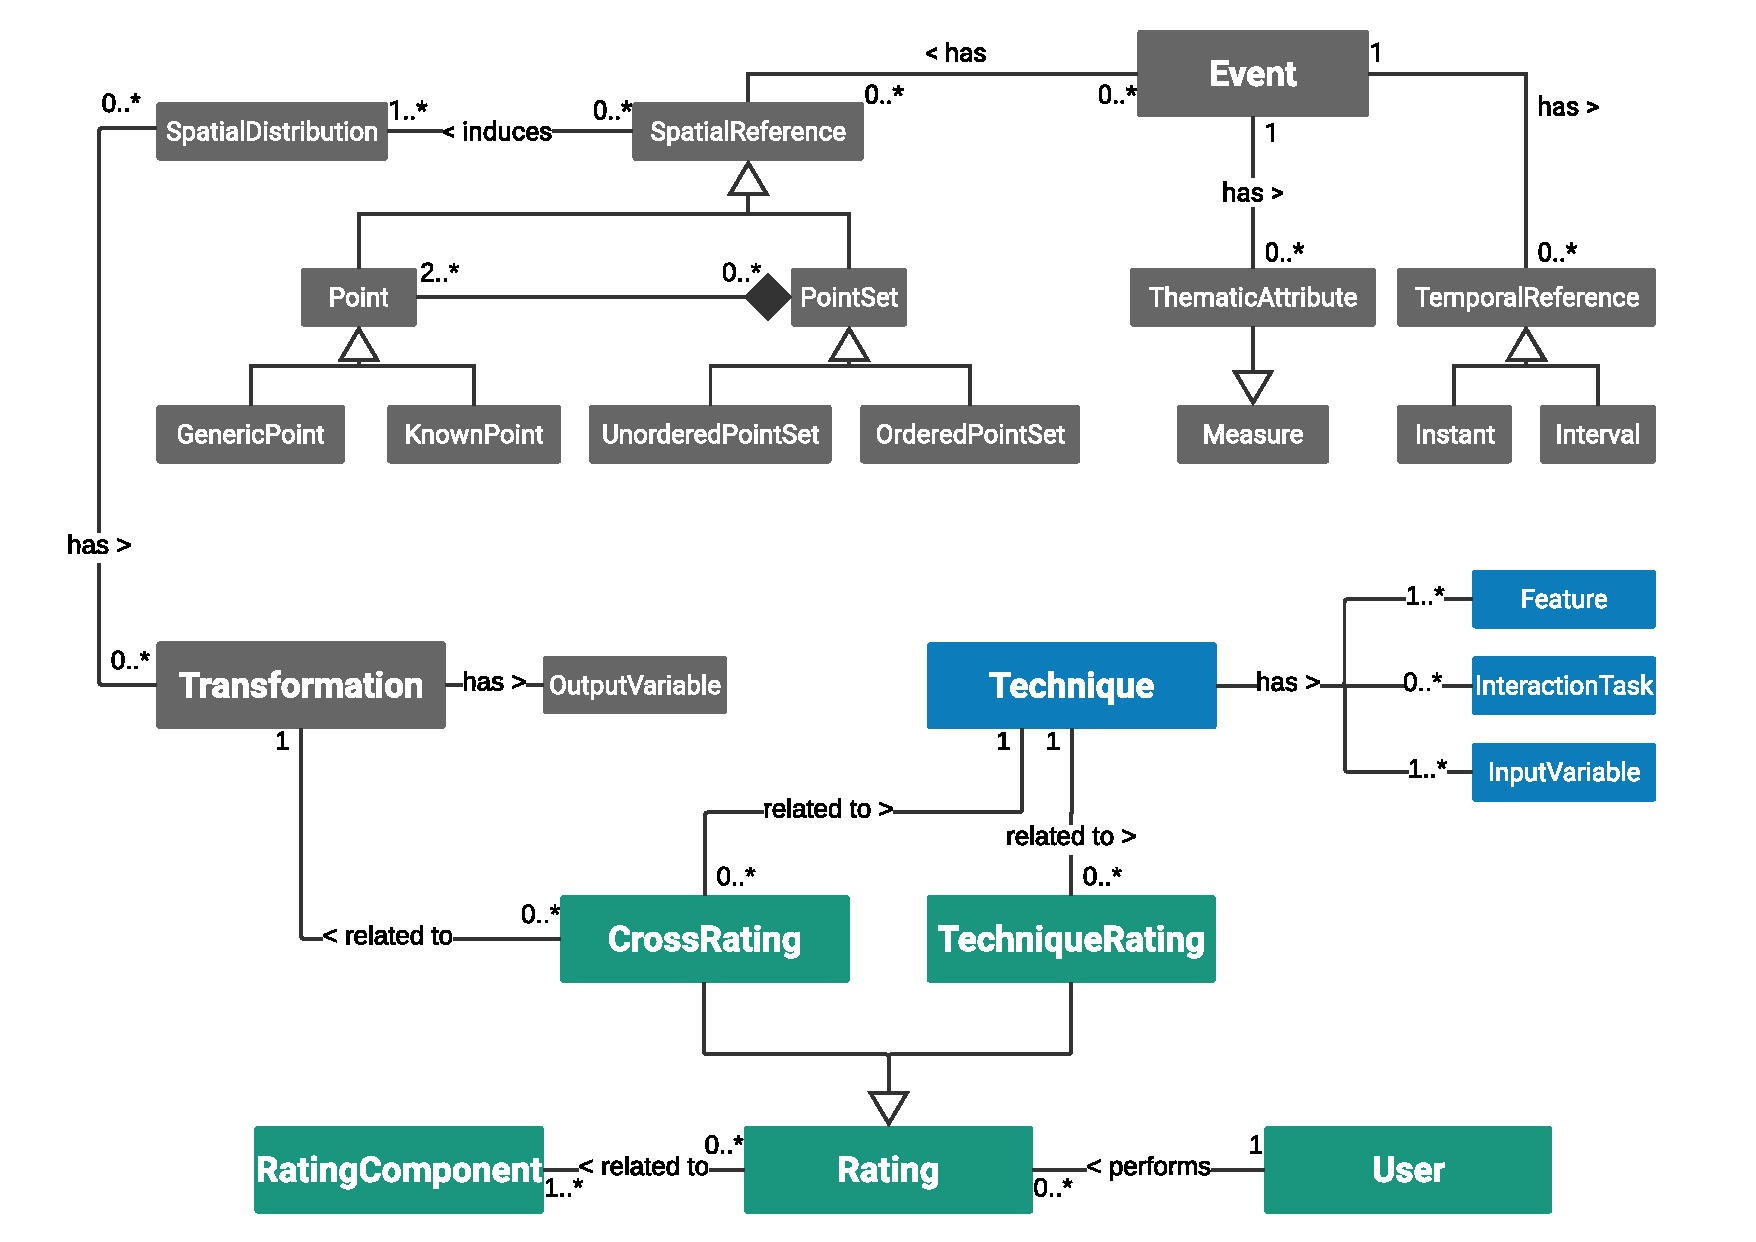
\includegraphics[width=15cm]{images/uml2018}
%	\caption{Schematic representation of an event as a UML Class Diagram. Classes are part of the conceptual model.}
%	\label{fig:uml}
%\end{figure}
%
%%An entity-based perspective was adopted, hence space and time were defined as attributes of every entity. The choice is justified by the structure of semantic data: every entity is an instance that exists per se, and it is described in terms of its attributes.
%
%An \textit{Event} contains spatial and temporal attributes (references), and thematic attributes. Spatial references are divided into two categories: \textit{Point} and \textit{PointSet}. Temporal references can be an \textit{Instant} or \textit{Interval}. Thematic attributes provide context about an entity.
%
%\subsection{Spatial References}
%\label{subsec:spatialreferences}
%
%A \textit{Point} is minimally described by latitude and longitude attributes. This definition is flexible in the sense that other optional attributes may exist, e.g. elevation. Points are divided into two disjoint subcategories: \textit{GenericPoint} and \textit{KnownPoint}.
%
%A \textit{GenericPoint} is a \textit{Point} that does not contain any thematic attribute that acts as an identifier. A \textit{KnownPoint} contains at least one identifier attribute.
%
%\textit{GenericPoint}s are references that, in practice, do not require identification, e.g. the location of a citizen at a given time, retrieved from a GPS-assisted device. \textit{KnownPoint}s are those for which the identification is relevant. For instance, the bus stops of a network are \textit{KnownPoint}s, as it is possible to retrieve their spatial references by knowing their identification, e.g., \textit{STCP\_AEPT1}.
%
%A \textit{PointSet} is an (un)ordered collection of two or more \textit{Point}s. \textit{PointSet}s are divided into two subcategories: \textit{UnorderedPointSet} and \textit{OrderedPointSet}. In contrast to a \textit{Point}, the disjointness assumption is not imposed for two reasons: (1) to account for situations where the notion of order or its absence is semantically irrelevant, and (2) to reduce computational complexity at inference time with VUMO rules.
%
%An \textit{OrderedPointSet} $P$ is well-ordered, i.e. every non-empty subset of $P$ has a least element in this ordering. An \textit{UnorderedPointSet} is a set of points that is not well-ordered.
%
%%An \textit{OrderedPointSet} has points ordered according to attributes that form a relation of order.
%
%An example of \textit{OrderedPointSet} is a passenger route plan, formed by \textit{Point}s which describe the departure and arrival locations. It is possible to infer the rank of any \textit{Point}. In contrast, shapes can be described in terms of \textit{UnorderedPointSet}s, e.g., a set of \textit{Point}s which defines the boundaries of a polygon representing a public transportation system zone.
%
%\subsection{Spatial Distributions}
%
%Spatial references induce distinct visual arrangements, according to their type. Such arrangements are defined Spatial Distributions. Three primary arrangements are considered: \textit{Discrete}, \textit{Quasi-continuous} and \textit{Graph}. Without loss of generality, spatial distributions are present in both geographic and abstract space. Spatial arrangements become apparent as the number of entities increase in visualization space, as shown in Fig. \ref{fig:spatialdistribution}. The following axioms are defined to link spatial reference types to distributions:
%
%\begin{figure}[!t]
%\centering
%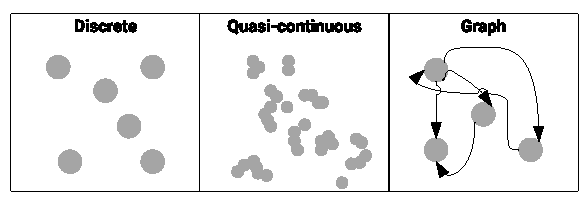
\includegraphics[width=9.2cm]{images/spatialdistribution.pdf}
%\caption{Examples of Discrete, Quasi-continuous and Graph spatial distributions in visualization space.}
%\label{fig:spatialdistribution}
%\end{figure}
%
%\textit{A1}: A \textit{KnownPoint} induces a \textit{Discrete} spatial distribution. The requirement of one or more identifier attributes suggest that \textit{KnownPoint}s represent entities that have a well-defined location within a region, and are less dense than \textit{GenericPoint}s.
%
%\textit{A2}: A \textit{GenericPoint} induces a \textit{Quasi-continuous} spatial distribution. Given that \textit{GenericPoint}s are not identified, they are suitable for representing entities that may be within a broader region in space. Thus, the visual behavior of \textit{Point}s induces a smooth, quasi-continuous arrangement.
%
%\textit{A3}: An \textit{UnorderedPointSet} induces a \textit{Discrete} spatial distribution. \textit{UnorderedPointset}s yield structures such as shapes and clusters, which are well defined in visualization space.
%
%\textit{A4}: An \textit{OrderedPointSet} induces a \textit{Graph} spatial distribution. They form arrangements that resemble the notion of trajectory.
%
%A \textit{PointSet} inherits the spatial distributions induced by its \textit{Point}s. In other words, \textit{PointSet}s also induce \textit{Discrete} and/or \textit{Quasi-continuous} spatial distributions, according to the types of \textit{Point}s in a set. The practical purpose of this definition is to account for situations in which a visualization provides mechanisms to not only explore \textit{PointSet}s as a whole, but to shift the perspective to its elements, using interaction mechanisms like semantic zoom.
%
%\subsection{Temporal References}
%
%An \textit{Event} has one or more temporal references of the following types: \textit{Instant} and \textit{Interval}. An \textit{Instant} is described by a timestamp, and optional parameters, e.g. time zone. An \textit{Interval} contains two timestamps corresponding to its beginning and end.
%
%\subsection{Thematic Attributes and Measures}
%\label{subsec:thematicattributes}
%
%Thematic attributes may be strings or numerical values. If an attribute has a numerical type, it introduces an intrinsic \textit{Measure} to an \textit{Event}. Examples of measures include the number of injured people in an accident, or the number of availale bikes at a docking station.
%
%\subsection{Data Transformations}
%\label{subsec:datatransformations}
%
%Data transformations, e.g., queries, provide additional information that is not explicit in raw data. The output of transformations may return new entities and values as a result of various operations. For instance, a transformation may use raw data to return the number of ticket validations that occurred on a given bus route during a time period.
%
%Part of the output may consist of spaital references, and measures derived from raw data. A transformation may inherit visual arrangements according to the spatial reference types. In fact, let $T$ be a transformation with $\{t_1,...,t_n\}$ as output variables, where $T_s \subseteq T$ is a non-empty subset of $T$ containing spatial references, with $1 \leq i \leq n$. By definition, a spatial reference $t_i$ induces one or more spatial distributions, hence the output of $T$ also induces one or more spatial distributions. % Ts C T.

%\section{The VUMO Ontology}
%\label{sec:vumo}
%
%VUMO is a urban mobility ontology that implements the conceptual model described in Section \ref{sec:conceptualmodel}. Given the orientation towards data visualization, it allows for the semantic annotation of visualization techniques and expert knowledge. The ontology is developed in Web Ontology Language (OWL) according to the OWL 2 RL profile, which is a syntatic subset of OWL 2 that supports rule-based inference \citep{owl}.
%
%%The re-use of existing ontologies is a desirable practice, as it enhances interoperability of existing semantic data. The following ontologies are used by VUMO:
%
%%\begin{itemize}
%%\item Basic Geo Vocabulary (\textit{geo}): represents information about "latitude, longitude and spatially-located things, using WGS84 as a reference datum";
%%\item Semantic Sensor Networks (\textit{ssn}): represents information about sensors, their properties and readings;
%%\item General Transit Feed Specification (\textit{gtfs}): describes structural information of PTSs, e.g. stops, routes, schedule and fares.
%%\end{itemize}
%
%%VUMO provides a set of rules to (1) infer implicit information in data, (2) derive visualization-related features from data and transformations, based on the conceptual model defined in Section \ref{sec:conceptualmodel}, and (3) to infer compatibility of a visualization with one or more transformations.
%
%Inference rules are expressed as SPARQL queries with the SPARQL Inference Notation (SPIN) vocabulary.  SPIN also provides an API built on top of Apache Jena, a framework for developing ontology-based applications with inference support. Subsection \ref{subsec:rules} describes VUMO rules.
%
%%Inference rules are expressed with the SPARQL Inference Notation (SPIN) vocabulary. SPIN is a vocabulary that provides an API built on top of Apache Jena, a framework for developing ontology-based applications. Subsection \ref{subsec:rules} describes VUMO rules. Subsection \ref{subsec:rules} describes VUMO rules.
%
%By design, it is proposed that recommendation algorithms evaluate two criteria: \textit{compatibility} and \textit{appropriateness}. Compatibility ensures that it is possible to visually encode the output of a transformation. Appropriateness enriches the quality of recommendations by processing expert knowledge.% VRSs are expected to implement recommendation algorithms to measure the latter criterion.
%
%\setcounter{table}{1}
%\begin{sidewaystable*}
%%\begin{table*}[ht!]
%	%\renewcommand{\arraystretch}{1.3}
%	\caption{Upper classes of VUMO and their respective first-level subclasses}
%	\label{tab:vumoconcepts}
%	\centering
%	\begin{tabular}{c|l|p{11cm}}
%		\hline
%		Upper class  &  Subclass & Definition\\
%		\hline
%		\hline
%		
%		\multirow{5}{*}{\textit{\shortstack{Urban\\ Mobility\\ Concept \\(UMC)}}}   &   \textit{Agent} & - An entity capable of triggering actions, e.g. \textit{Event}s.\\
%		& \textit{InfrastructureComponent} & - A physical or abstract entity. \textit{Agent}s can use it (in)directly trigger \textit{Event}s, or to provide them with context information.\\
%		& \textit{Event} & - An action performed by one or more \textit{Agent}s, which may take place in multiple space and time dimensions.\\
%		\hline
%		
%		\multirow{4}{*}{\textit{\shortstack{Data\\Concept\\(DC)}}}    &   \textit{SpatialReferenceType}	&	- A type of spatial reference.\\
%		&	\textit{TemporalReferenceType}	& - A type of temporal reference. \\
%		&	\textit{SpatialDistribution}	& - A type of visual arrangement of spatial data. \\
%		&	\textit{Transformation} & - A sequence of operations (e.g. query) that yields new information from raw data.  \\
%		
%		\hline
%		\multirow{3}{*}{\textit{\shortstack{Visualization\\Concept\\(VC)}}}	&	\textit{Technique}	& - A visualization technique available in a VUMO-based VRS.\\
%		&	\textit{Feature}	& - An intrinsic characteristic of a \textit{Technique}. \\
%		&	\textit{InteractionTask}	& - An interaction mechanism available in a \textit{Technique}. \\
%		
%		\hline
%		
%		\multirow{12}{*}{\textit{\shortstack{Domain\\Expert\\Concept\\(DEC)}}}		&	\textit{DomainExpert}	& - A user of a VUMO-based VRS. \\
%		&	\textit{DomainExpertProfile}	& - The profile of a \textit{DomainExpert} with respect to the context of his/her activities, e.g. \textit{Strategic}, \textit{Operational}. \\
%		&	\textit{TechniqueRating}	& - An abstract container that stores rating information made by a \textit{DomainExpert} with respect to a \textit{Technique}. \\
%		&	\textit{RatingCriteria}		& - An abstract component evaluated in a rating that impacts the user experience, e.g. \textit{Difficulty}, \textit{Visual clutter}. Such components are divided into \textit{Positive/NegativeRatingCriteria}. \\
%		&	\textit{CrossRating}	& - An abstract container that stores rating information about a \textit{Technique} with respect to a \textit{Transformation}. A \textit{CrossRating} provides a specialized rating in comparison to a \textit{TechniqueRating}, which does not depend on a \textit{Transformation}. \\
%		&	\textit{AnalyticalTask}	& - An exploratory data analysis task performed by a \textit{DomainExpert}, e.g. ridership analysis. A task is associated with one or more \textit{Transformation}s. \\
%		
%		\hline
%	\end{tabular}
%%\end{table*}
%\end{sidewaystable*}
%
%Four upper classes are defined:
%
%\begin{itemize}
%	\item \textit{UrbanMobilityConcept (UMC)}: concepts that describe public transportation systems and spatial events.
%	\item \textit{DataConcept (DC)}: concepts from the conceptual model (Section \ref{sec:conceptualmodel}).
%	\item \textit{VisualizationConcept (VC)}: concepts for the annotation of visualization techniques, their properties and interaction tasks.
%	\item \textit{DomainExpertConcept (DEC)}: concepts for the annotation of domain experts that would use a VRS, their empirical knowledge about the visualization techniques.
%\end{itemize}
%
%Upper classes branch out into subclasses that represent more specific concepts. VUMO contains Object and Datatype properties to relate instances from the aforementioned classes. Semantic data is herein represented using the standard form, i.e. subject-predicate-object triples, according to the Resource Description Framework (RDF) data model. Table \ref{tab:vumoconcepts} provides a natural language definition for each first-level subclass.
%
%A symbolic notation was adopted for representing semantic data: classes ($\blacksquare$) and their instances ($\blacklozenge$). Object and Datatype properties are represented by blue and green edges. Solid and dashed edges indicate asserted (explicit) and inferred (implicit) triples, respectively. Throughout the text, classes, properties and instances are written in italic, e.g. \textit{ns:semanticThing}, where the prefix \textit{ns} indicates the namespace, i.e. the ontology in which the property is defined. For instance, \textit{geo} is the prefix of the Basic Geo vocabulary, which is used to describe spatial coordinates \citep{Brickley2003}. No prefix is used for VUMO components.
%
%\subsection{UrbanMobilityConcept (UMC)}
%
%UMC concepts are fundamental to semantic integration of raw data. The \textit{Agent} and \textit{InfrastructureComponent} subclasses describe structural concepts of a public transportation system. \textit{Event} describes distinct types of spatial events. Table \ref{tab:umc} describes UMC and its components.
%
%
%\setcounter{table}{1}
%\begin{sidewaystable}
%%\begin{table*}[ht!]
%	%\renewcommand{\arraystretch}{1.3}
%	\caption{First-level and further subclasses of UrbanMobilityConcept (UMC)}
%	\label{tab:umc}
%	\centering
%	\begin{tabular}{c|l|p{12cm}}
%		\hline
%		Subclass  &  Second-level subclass & Definition and further subclasses (if applicable)\\
%		\hline
%		\hline
%		
%		\multirow{3}{*}{\textit{Agent}}   &   \textit{Operator} & - A transportation operator, e.g. bus or subway companies).\\
%		& \textit{Passenger} & - An individual who uses a public transportation system. \\
%		& \textit{Vehicle} & - An action performed by one or more \textit{Agent}s, which may take place in multiple space and time dimensions.\\
%		\hline
%		
%		\multirow{7}{*}{\textit{\shortstack{Infrastructure\\Component}}}    &  \textit{Line}	& - A PTS line that may consist of various \textit{Route}s.\\
%		&	\textit{Node} &	- A node of the transportation network graph, e.g. \textit{BusStop}, \textit{SubwayStation}, \textit{Sensor}.\\
%		&	\textit{PTSZone}	& - A zone defined by a transportation network for a certain purpose, e.g. to define fares. \\
%		&	\textit{Route} & - A path followed by a \textit{Line}. \\
%		&	\textit{RouteSegment} & - A part of a \textit{Route}, generally defined by two \textit{Node}s. \\
%		&	\textit{Ticket}	& - A ticket that allows a passenger to travel within a public transportation network. \\
%		&	\textit{TicketType} & - The type of a ticket.  \\
%		
%		\hline
%		\multirow{8}{*}{\textit{Event}}	&	\textit{TravelEvent}	& - A travel made by a passenger within a transportation network triggered by an action, e.g. \textit{TicketValidation}, \textit{BicycleHire}.\\
%		&	\textit{TravelIntention}	& - An intention of traveling within a transportation network, based on information requests, e.g. schedule requests or route plans. \\
%		&	\textit{SensorReading}		& - A reading made by a \textit{Sensor}. \\
%		&	\textit{SocialMediaPost}	& - A post from social media regarding transportation information. \\
%		&	\textit{TripEvent}	&	- A trip made by a \textit{Vehicle}, e.g. bus or taxi). \\
%		&	\textit{UnexpectedEvent}	& - An unforeseen \textit{Event}, often capable of (partly) disrupting a transportation network in some way. \\
%		
%		\hline
%	\end{tabular}
%%\end{table*}
%\end{sidewaystable}
%
%
%\subsection{DataConcept (DC)}
%
%DC implements the conceptual model defined in Section \ref{sec:conceptualmodel}. The \textit{SpatialReferenceType} subclass is refined into \textit{Point} (\textit{GenericPoint} and \textit{KnownPoint}) and \textit{PointSet} (\textit{UnorderedPointSet} and \textit{OrderedPointSet}). \textit{TemporalReferenceType} contains two subclasses: \textit{Instant} and \textit{Interval}. The \textit{SpatialDistribution} class contains three instances: \textit{Discrete}, \textit{Quasi-continuous} and \textit{Graph}. Axioms A1 to A6 are also implemented as triples.
%
%To instantiate a \textit{Point}, the properties \textit{geo:lat} and \textit{geo:long} are used. If applicable, an identification can be defined with \textit{hasID} or its semantically equivalent subproperties available in VUMO, such as \textit{hasInternalID} or \textit{hasFriendlyID}. To illustrate the utility of multiple ID properties, consider the bus stop shown in Fig. \ref{fig:stcp_stop} from the city of Porto. \textit{AEPT1} is a user friendly identification used by passengers to consult schedules using real time services. From the operator's perspective, one or more identifications can be used, such as \textit{STCP\_AEPT1} or \textit{54}. All IDs uniquely determine the stop within their distinct semantic contexts.
%
%\begin{figure}[!t]
%	\centering
%	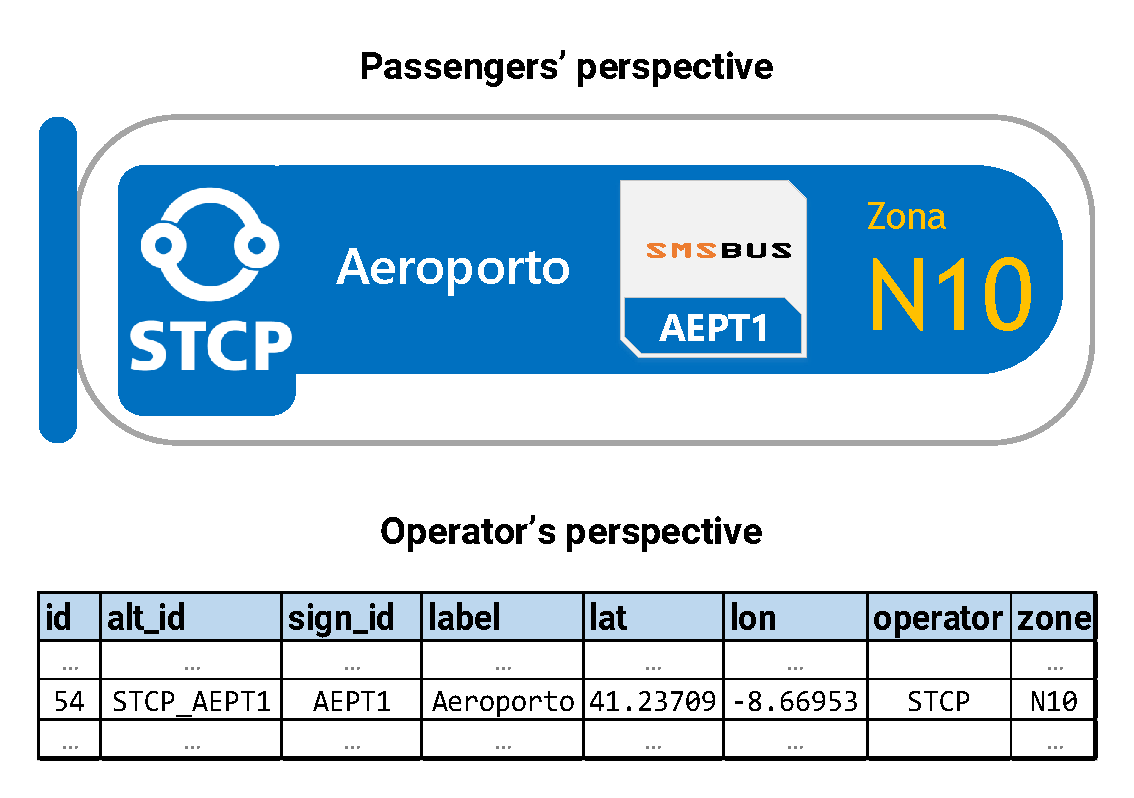
\includegraphics[width=7cm]{images/stop.pdf}
%	\caption{A bus stop of STCP bus operator in Porto. The identification AEPT1 is meant to be used by passengers when checking schedules in a real-time service.}
%	\label{fig:stcp_stop}
%\end{figure}
%
%If a \textit{PointSet} is subject to a relation of order, properties such as \textit{hasOrigin} and \textit{hasDestination} are available, as they are subproperties of \textit{hasOrderedSpatialReference}. Otherwise, properties that are not subject to a relation of order should be used, such as \textit{hasZoneBoundaryPoint} or \textit{hasPoint}, which are equivalent subproperties of \textit{hasUnorderedSpatialReference}.
%
%Measures are defined as subproperties of \textit{hasMeasure}, such as \textit{hasNumberOfInjuredPassengers} and \textit{hasNumberOfAvailableBicycles}, which can describe, for example, an \textit{Accident} or the status of \textit{BicycleStation}.
%
%Data transformations are modeled as instances of \textit{Transformation}, and their queries can be expressed in SPARQL. The SPIN vocabulary allows queries to be stored within the ontology. Moreover, rules analyze transformations to infer characteristics such as spatial distribution or compatibility with visualization techniques. Subsection \ref{subsec:rules} also describes how rules are applied to \textit{Transformation}s.
%
%\subsection{VisualizationConcept (VC)}
%
%VC allows for the annotation of visualization techniques. The \textit{Technique} class is used to create instances that represent the techniques of a VRS. \textit{InteractionTask} refers to interactive features of a mechanisms that a technique provides, e.g. \textit{SemanticZoom} or \textit{Filtering}. \textit{Feature} comprises intrinsic components related to the grapical and data aspects of visualizations. The following subclasses of \textit{Feature} are defined:
%
%\begin{itemize}
%	\item \textit{ReferenceFrame}: the type of visualization space, e.g. \textit{Abstract}, \textit{Geographic};
%	\item \textit{SpatialDimensionality}: the number of spatial dimensions used to represent data, e.g. \textit{2D}, \textit{3D};
%	\item \textit{TemporalRepresentation}: the mode with which time is depicted in a visualization technique, e.g. \textit{Static}, \textit{Dynamic};
%	\item \textit{InputVariable}: a variable that receives values from an output variable and maps it onto a visual feature, e.g. color hue/saturation or shape size. VUMO rules analyze \textit{InputVariable}s to evaluate the compatibility of between \textit{Technique}-\textit{Transformation} pairs.
%\end{itemize}
%
%%Visualization techniques are seldom immutable representations of data. Interaction tasks provide means of manipulating visualizations, such as zooming or filtering.
%
%\subsection{DomainExpertConcept (DEC)}
%
%DEC allows for the annotation of urban mobility experts knowledge. Such knowledge serve as input to recommendation algorithms to assess \textit{appropriateness} of visualizations. Experts (system users) are represented as instances of \textit{DomainExpert}, each one having a \textit{DomainExpertProfile}, e.g. \textit{Strategic} or \textit{Operational}. 
%
%\textit{DomainExpert}s would use a VRS to carry \textit{AnalyticalTask}s, e.g. "\textit{Ridership and travel intentions to bus stops within a public transportation system zone}". An \textit{AnalyticalTask} consist of one or more \textit{Transformation}s that contain the queries to be executed.
%
%\textit{TechniqueRating}s are statements made by \textit{DomainExpert}s about a \textit{Technique}. A \textit{TechniqueRating} contain one or more statements regarding \textit{RatingComponent}s, which are specified according to the requirements of a VRS. For instance, a \textit{TechniqueRating} may assign a score of "5" to a \textit{Technique} with respect to \textit{VisualClutter}, and state that it is recommended to visualize data related to \textit{TicketValidation}s using the \textit{hasRecommendedTheme} property. 
%
%In distinction to existing VRS approaches, VUMO allows for the annotation of specialized ratings. \textit{CrossRating}s are used to rate a \textit{Technique} with respect to a \textit{Transformation}, according to one or more \textit{RatingComponent}s.
%
%\subsection{VUMO rules}
%\label{subsec:rules}
%
%%Rules infer implicit knowledge from instance data. Such knowledge facilitates data integration and extracts structural characteristics that are relevant to visualization. Most rules consist of direct implications of the conceptual model (Section \ref{sec:conceptualmodel}).
%
%Rules \textit{R1} and \textit{R2} detect spatial references within instance data and infer their type, i.e. \textit{Point}s, \textit{PointSet}s, and their subtypes. Rules \textit{R3}, \textit{R4} and \textit{R5} infer characteristics of \textit{Transformation} queries based on their structure, namely: spatial distribution (\textit{R3}), themes (\textit{R4}), and use of aggregate functions (\textit{R5}).
%
%\textit{R3} analyzes conditional clauses for predicates containing  equivalent subproperties of \textit{:hasSpatialReference}. If one or more clauses satisfy that condition, the range of such property is used to retrieve the spatial reference type. The corresponding axiom is then used to retrieve the spatial distribution. %For instance, it follows from \textit{A1} that the query in Fig. X induces a \textit{Discrete} spatial distribution, as the property \textit{occursAtNode} has \textit{KnownPoint} as its range, by definition.
%
%\textit{R4} extracts themes, i.e. tags, that describe the urban mobility concepts related to a \textit{Transformation}. The rule finds condition clauses whose properties' ranges are subclasses of \textit{UrbanMobilityConcept}. Themes provide a natural language description of the contents of a \textit{Transformation}.
%
%\textit{R5} verifies if a \textit{Transformation} returns aggregate data, i.e. if at least one \textit{OutputVariable} contains an aggregate function. Such verification occurs while evaluating compatibility, as a \textit{Technique} may expect disaggregate instance data to perform aggregations externally.
%
%\textit{R6} evaluates the compatibility of a \textit{Transformation} with respect to a \textit{Technique}. Compatibility holds if the aggregate requirements (\textit{R5}) match, and if there exists at least one bijective mapping $m$ such that
%
%%\begin{align}
%\begin{align*}
%	m \colon & O^{\prime} \subseteq O \rightarrow I \\
%	& o_j \longmapsto i_k
%\end{align*}
%
%and $\theta(o_j) = \theta(i_k) \ \forall (o_j,i_k)$, where $o_j \in O^{ \prime}$ and $i_k \in I$ are the output and input variables, respectively. The $\theta$ operator retrieves the type of a variable, e.g. string, integer, instance.
%
%\begin{table}[ht!]
%%\renewcommand{\arraystretch}{1.3}
%\caption{Pseudocode representation of VUMO rules}
%\label{tab:rules}
%\centering
%\begin{tabular}{p{0.3cm}l}
%    \hline
%    \hline
%    Rule& Pseudocode\\
%    \hline
%
%	\multirow{7}{*}{R1} & // R1 infers \textit{Point}s and their subtypes \\
%	& $s \leftarrow \text{instance}$ // receives an instance  \\
%	&  \textbf{if} \textit{containsLatitudeLongitude($s$)} \textbf{then} \\
%	& \quad \textbf{if} \textit{containsIdentification($s$)} \textbf{then}\\
%	& \quad \quad $s \in \text{\textit{KnownPoint}}$ // infers $s$ as an instance of \textit{KnownPoint} \\
%	& \quad \textbf{else} \\
%	& \quad \quad $s \in \text{\textit{GenericPoint}}$ // infers $s$ as an instance of \textit{GenericPoint}\\
%	\hline
%	\multirow{8}{*}{R2} & // R2 infers \textit{PointSet}s and their subtypes \\
%	&  $s \leftarrow \text{instance}$  \\
%	& $P \leftarrow \bigcup_{s} p$ // Points referred by $s$, if any\\
%	&  \textbf{if} $|P| \geq 2$  \textbf{then} // $P$ should have at least two Points \\
%	& \quad \textbf{if} \textit{isOrdered($P$)} \textbf{then}\\
%	& \quad \quad $P \in \text{\textit{OrderedPointSet}}$ // infers $P$ is an \textit{OrderedPointSet} \\
%	& \quad \textbf{else} \\
%	& \quad \quad $P \in \text{\textit{UnorderedPointSet}}$ // infers $P$ is an \textit{UnorderedPointSet} \\
%	\hline
%	\multirow{9}{*}{R3} & // R3 infers \textit{SpatialDistribution}s of a \textit{Transformation}\\
%	&  $t \leftarrow \text{instance}$, $q_t \leftarrow \text{query within } t$, such that $t \in \text{\textit{Transformation}}$ \\
%	& $C \leftarrow \bigcup_{q_t} c$ // condition clauses of $q_t$\\
%	&  \textbf{for each} $c \in C$ \textbf{do} \\
%	& \quad $p_c \leftarrow \text{\textit{property(}}c\text{\textit{)}}$ // receives the property (predicate) of $c$ \\
%	& \quad \textbf{if} $p_c \equiv \text{\textit{hasSpatialReference}}$ \textbf{then} \\
%	& \quad \quad $r_{p_c} \leftarrow \text{\textit{range(}}p_c\text{\textit{)}}$ // receives the range of property $p_c$ \\
%	& \quad \quad $\sigma_{r_{p_c}} \leftarrow \text{\textit{getSpatialDistribution(}}r_{p_c}\text{\textit{)}}$ \\
%	& \quad \quad $t$ \textit{hasSpatialDistribution} $\sigma_{r_{p_c}}$ // inferred triple\\
%	\hline
%	\multirow{8}{*}{R4} & // R4 infers themes (tags) of a \textit{Transformation}\\
%	&  $t \leftarrow \text{instance}$, $q_t \leftarrow \text{query within } t$, such that $t \in \text{\textit{Transformation}}$ \\
%	& $C \leftarrow \bigcup_{q_t} c$ // condition clauses in $q_t$\\
%	&  \textbf{for each} $c \in C$ \textbf{do} \\
%	& \quad $p_c \leftarrow \text{\textit{property(}}c\text{\textit{)}}$ // receives the property (predicate) of $c$ \\
%	& \quad \textbf{if} $\text{\textit{range(}}p_c\text{\textit{)}} \equiv \text{\textit{UrbanMobilityConcept}}$ \textbf{then} \\
%	& \quad \quad $r_{p_c} \leftarrow \text{\textit{range(}}p_c\text{\textit{)}}$ // receives the range of property $p_c$ \\
%	& \quad \quad $t$ \textit{hasTheme} $r_{p_c}$ // inferred triple\\
%	\hline
%	\multirow{9}{*}{R5} & // R5 infers if the query of a \textit{Transformation} returns aggregate results\\
%	&  $t \leftarrow \text{instance}$, $q_t \leftarrow \text{query within } t$, such that $t \in \text{\textit{Transformation}}$ \\
%	& $V \leftarrow \bigcup_{q_t} v$ // set of output variables of $q_t$\\
%	&  \textbf{for each} $v \in V$ \textbf{do} \\
%	& \quad \textbf{if} $\text{\textit{isAggregate(}}v\text{\textit{)}}$ \textbf{then} \\
%	& \quad \quad $t$ \textit{returnsAggregateResults} \textit{true} // inferred triple\\
%	& \quad \quad \textbf{break} // one occurrence is sufficient \\
%	& \quad \textbf{else} \\
%	& \quad \quad $t$ \textit{returnsAggregateResults} \textit{false} // inferred triple\\
%	\hline
%	\multirow{9}{*}{R6} & // R6 infers compatibility of a \textit{Transformation}-\textit{Technique} pair \\
%	& $t,v \leftarrow$ instances, such that $t \in \text{\textit{Transformation}}, v \in \text{\textit{Technique}}$ \\
%	& $O,I \leftarrow \text{output and input variables sets of $t$, respectively}$\\
%	& $\xi \leftarrow \varnothing$ // result set of compatible mappings \\
%	& \textbf{if} \textit{meetsAggregateRequirements}($t,v$) \textbf{then} \\
%	& \quad \textbf{if} $\text{\textit{range(}}p_c\text{\textit{)}} \equiv \text{\textit{UrbanMobilityConcept}}$ \textbf{then} \\
%	& \quad $\xi \leftarrow \text{\textit{findMapping(}}t,v\text{\textit{)}}$ // stores compatible mappings in $\xi$ \\
%	&\quad \textbf{if} $|\xi|\geq 1$ \textbf{then}\\
%	&\quad \quad $t$ \textit{isCompatibleWith} $v$ // inferred triple \\
%    \hline
%    \hline
%\end{tabular}
%\end{table}
%
%Table \ref{tab:rules} provides the pseudocode representation of rules R1-6. Inferred triples are represented with a specific notation. For instance, $s \in \mbox{\textit{GenericPoint}}$ is equivalent to "$s$ is an instance of \textit{GenericPoint}"; $t \mbox{\textit{ isCompatibleWith }} v$ denotes a subject-predicate-object triple.
%
%
%%VUMO provides a set of rules that support data integration and visualization recommendation. Rules were built with the SPIN vocabulary, thus they are specified as SPARQL queries. Ontologies that require rule-based reasoning are classified as OWL-RL ontologies. Focus is given to rules that are relevant for visualization. Reasoning over instance data occurs after data integration.
%
%%The conceptual model defined in Section \ref{sec:conceptualmodel} provides the basis for rules that extract features from data. Rules \textit{R1} and \textit{R2} infer whether an instance is a Point or PointSet, respectively, and to which subclass they belong. As shown in Fig. \ref{subfig:rule_point} and \ref{subfig:rule_pointset}, 
%
%%The SPIN vocabulary allows the definition of \textit{Transformation} queries as an RDF graph. The following rules consist of meta-queries that infer features from \textit{Transformation}s that are relevant for visualization techniques, based on the content and structure of queries. Two rules were implemented to infer spatial distribution (\textit{\textit{R3}}) and themes (\textit{R4}).
%
%%\textit{R3} infer the spatial distribution(s) of a \textit{Transformation} based on the query conditions, specified within the WHERE clause. Each condition (a triple) is evaluated with respect to its predicate (property). If the property is a subproperty of \textit{hasSpatialReference}, the rule retrieves the range of such property, e.g. a Point. Finally, the rule retrieves the spatial distribution by consulting the respective axiom (A1-A4)
%
%%\begin{figure}[!tbp]
%%\centering
%%\includegraphics[width=5cm]{images/rule_spatialdistribution.png}
%%\caption{Rule \textit{R3} - Inference of spatial distributions of a \textit{Transformation}}
%%\label{fig:rule_spatialdistribution}
%%\end{figure}
%
%%\textit{R4} infers the urban mobility concepts related to a \textit{Transformation}. For instance, a query may regard \textit{Event}s such as \textit{TicketValidation}s and \textit{ScheduleRequest}s. Such themes work as tags that can be used by recommendation algorithms. \textit{R4} evaluates whether the conditions contain a predicate that expects an \textit{UrbanMobilityConcept} as a predicate. If it does, the concept is related to the transformation with the \textit{hasTheme} property.
%
%%R5 is an auxiliary rule for inferring whether a query returns aggregated data, i.e. according to an aggregate function, e.g. COUNT(), SUM(). Given that a visualization techniques may be developed to perform data aggregation, such information is important for evaluating compatibility. The rule evaluates whether a query contains an aggregate function, which should be followed by a GROUP BY statement. The \textit{Transformation} receives a new triple using the property \textit{returnsAggregatedData}, which can be \textit{true} or \textit{false}.
%
%%Rule R6 evaluates whether a \textit{Transformation} is compatible with a \textit{Technique}. The first condition verifies if the number of output variables of a \textit{Transformation} is lower than the number of non-optional input variables of a \textit{Technique}. If not, the second condition verifies is there is at least one mapping between variables, i.e. if every \textit{OutputVariable} is mapped onto an \textit{InputVariable} of the same tipe, e.g. numeric. The \textit{Transformation} receives a new triple with predicate \textit{isCompatibleWithTechnique} in case the condition is satisfied.
%
%%\begin{figure}
%%\centering
%%\subfloat[Rule \textit{R1} -\textit{Point} type inference\label{subfig:rule_point}]{\includegraphics[width=7cm]{images/rule_point.png}}
%%\\
%%\subfloat[Rule \textit{R2} - \textit{Pointset} type inference\label{subfig:rule_pointset}]{\includegraphics[width=7cm]{images/rule_pointset.png}}
%%\caption{Rules for inferring \textit{Point}s (a) and \textit{Pointset}s (b)}
%%\label{fig:r1r2}
%%\end{figure}

\section{Practical Applications}
\label{sec:practical}

This section demonstrates VUMO applied to semantic integration of data, annotation of visualizations and expert knowledge. The supporting data is related to the public transportation system of Porto, Portugal, and provide information about (a) smart card ridership for bus and subway services, description of (b) stops and stations, (c) fare zones, (d) ticket types, and (e) usage data from Move-me schedule consultation service. Move-me is a mobile application that provides real-time information about Porto's public transportation system. Two prototypical visualization techniques were developed to support the demonstration. Expert knowledge was collected through exploratory usability tests with local domain experts, who are involved in strategic and operational decisions for the public transportation system. Two prototypical domain experts were defined based on such knowledge.

\subsection{Semantic integration of data}

Datasets were provided in various formats: CSV (a,b), Excel spreadsheets (c,d), and SQL dumps (e). The mapping of each dataset schema onto the VUMO classes and properties is supported by an \textit{ad hoc} parser which also returns semantic instance data in RDF. The resulting graph was stored in a triple store engine. Figure \ref{fig:rdfgraph} illustrates an excerpt of the resulting graph containing elements from original source data.

In particular, dataset (b) is described by the schema shown in Fig. \ref{fig:stcp_stop}, where each row corresponds to a stop. Table \ref{tab:correspondence} shows a possible mapping between the source attributes and VUMO properties.

As the RDF graph is independent of source data and their schemes, it is possible to manipulate data from all datasets simultaneously. For instance, \textit{TicketValidation301} and \textit{SchedReq12} have \textit{BusStop54} as a common spatial reference.

It follows from \textit{R1} and \textit{R2} that \textit{AEPT1} and \textit{N10} are \textit{KnownPoint} and \textit{OrderedPointSet}, respectively. \textit{TicketValidation301} and \textit{N10} are inferred as instances of \textit{TicketValidation} and \textit{Zone}, as they are the domain of properties \textit{hasValidationDateTime} and \textit{hasZoneBoundaryPoint}, respectively. Inferences related to domain and range are native to RDF semantics and do not require the specification of inference rules.

\begin{table}[ht!]
%\renewcommand{\arraystretch}{1.3}
\caption{Mapping between attributes of (b) and VUMO properties}
\label{tab:correspondence}
\centering
\begin{tabular}{lll}
    \hline
    \hline
    Source attribute & Target property & Property type\\
    \hline

	id & \textit{hasID} & Datatype\\
	alt\_id & \textit{hasID} & Datatype\\
	sign\_id & \textit{hasFriendlyID} & Datatype\\
	label & \textit{hasName} & Datatype\\
	lat & \textit{wgs84:lat} & Datatype\\
	lon & \textit{wgs84:lon} & Datatype\\
	operator & \textit{operatedBy} & Object\\
	zoneID & \textit{location} & Object \\
    \hline
    \hline
\end{tabular}
\end{table}

%\begin{figure}[!tbp]
%\centering
%\includegraphics[width=\textwidth]{images/rdf.pdf}
%\caption{Excerpt from RDF graph of mobility data from Porto Public Transportation System}
%\label{fig:instancedata}
%\end{figure}

\subsection{Visualization Knowledge and Data Transformations}

Map-based and abstract visualization techniques were developed: geographic (\textit{GeoHeatMap}) and calendar (\textit{CalHeatMap}) heat maps, respectively. The former depicts the density of instance data in geographic space. The latter depicts density in a daily arrangement. Each day is assigned to a color according to the number of occurrences.

\textit{GeoHeatMap} requires the following input variables: (a) an event instance; (b,c) spatial (latitude and longitude) and (c) temporal references (instant). Variable (a) receives the entity to be plotted, (b,c) provide the instance coordinates on a map, and (d) is used for temporal filtering. \textit{CalHeatMap} requires the same variables but (b,c). Semantic zoom is available in both techniques. By construction, \textit{CalHeatMap} require aggregate data. \textit{GeoHeatMap} does not. Fig. \ref{fig:vis_user} shows the semantic annotation of both visualization techniques.

\begin{figure}
\centering
\subfloat[Geographic heat map\label{subfig:geoheatmap}]{\includegraphics[width=8.5cm]{images/geoheatmap}}
\\
\subfloat[Calendar heat map\label{subfig:calheatmap}]{\includegraphics[width=8.5cm]{images/calheatmap}}
\caption{Prototypical visualization techniques compliant with VUMO}
\label{fig:visualizations}
\end{figure}

%Let \textit{porto:T1} and \textit{porto:T2} be two data transformations related to the domain task "Analysis of travel events and intentions". \textit{porto:T1} returns the total of ticket validations, the ID and geographic coordinates of each node during a given time period. \textit{porto:T2} returns the same data, except for the coordinates. Their respective SPARQL query formulation is given by Listing \ref{alg:transformation}. The query searches for a subgraph that matches the triple patterns related to events that occured at a given node. The COUNT() function aggregates the results by node.

Let \textit{AT1} be an instance of \textit{AnalyticalTask} described by "analysis of \textit{TicketValidation}s and \textit{ScheduleRequest}s", and \textit{T1} an instance of \textit{Transformation} that implements the following query with five output variables:

\begin{algorithmic}
  
 \label{alg:transformation1}

  \STATE \textbf{SELECT} \textit{?ev ?lat ?lon ?time} COUNT(\textit{?node}) AS \textit{?total}
  \STATE \textbf{WHERE \{}
  \STATE \hspace{5mm} \textit{?ev rdf:type (:TicketValidation OR :ScheduleRequest) .}
  \STATE \hspace{5mm} \textit{?ev time:inXSDDateTimeStamp ?time .}
  \STATE \hspace{11mm} \textit{location ?node .}
  \STATE \hspace{5mm} \textit{?nodeID wgs84:lat ?lat .}
  \STATE \hspace{18mm} \textit{wgs84:lon ?lon .}
  \STATE \hspace{5mm} \textbf{FILTER (}\textit{?time $\geq$ ?arg1} \&\& \textit{?time $\leq$ ?arg2}\textbf{) \}}
  \STATE {\textbf{GROUP BY} \textit{?node}}
\end{algorithmic}

\textit{AT1} is linked to \textit{T1} via the property \textit{hasRelatedTransformation}. An \textit{AnalyticalTask} can be linked to one or more \textit{Transformation}s. Arguments \textit{arg1} and \textit{arg2} are placeholder values that can be changed by the user.

From R4, it follows that \textit{T1} contains a \textit{Discrete} spatial distribution, as the property \textit{occursAtNode} has \textit{Node} as its range, which is defined as semantically equivalent to a \textit{KnownPoint}. R4 yields the tags \textit{TicketValidation} and \textit{ScheduleRequest}. It follows from R6 that \textit{T1} returns aggregate results due to the COUNT function.

It follows from R7 that \textit{T1} is compatible with \textit{CalHeatMap}, but not \textit{GeoHeatMap}, due to the aggregate results requirement. Consider another instance of \textit{Transformation}, \textit{T2}, that implements the same query as \textit{T1} except for the aggregate function. Hence, \textit{T2} is compatible with \textit{GeoHeatMap}, but not \textit{CalHeatMap}.

\begin{sidewaysfigure}
\centering
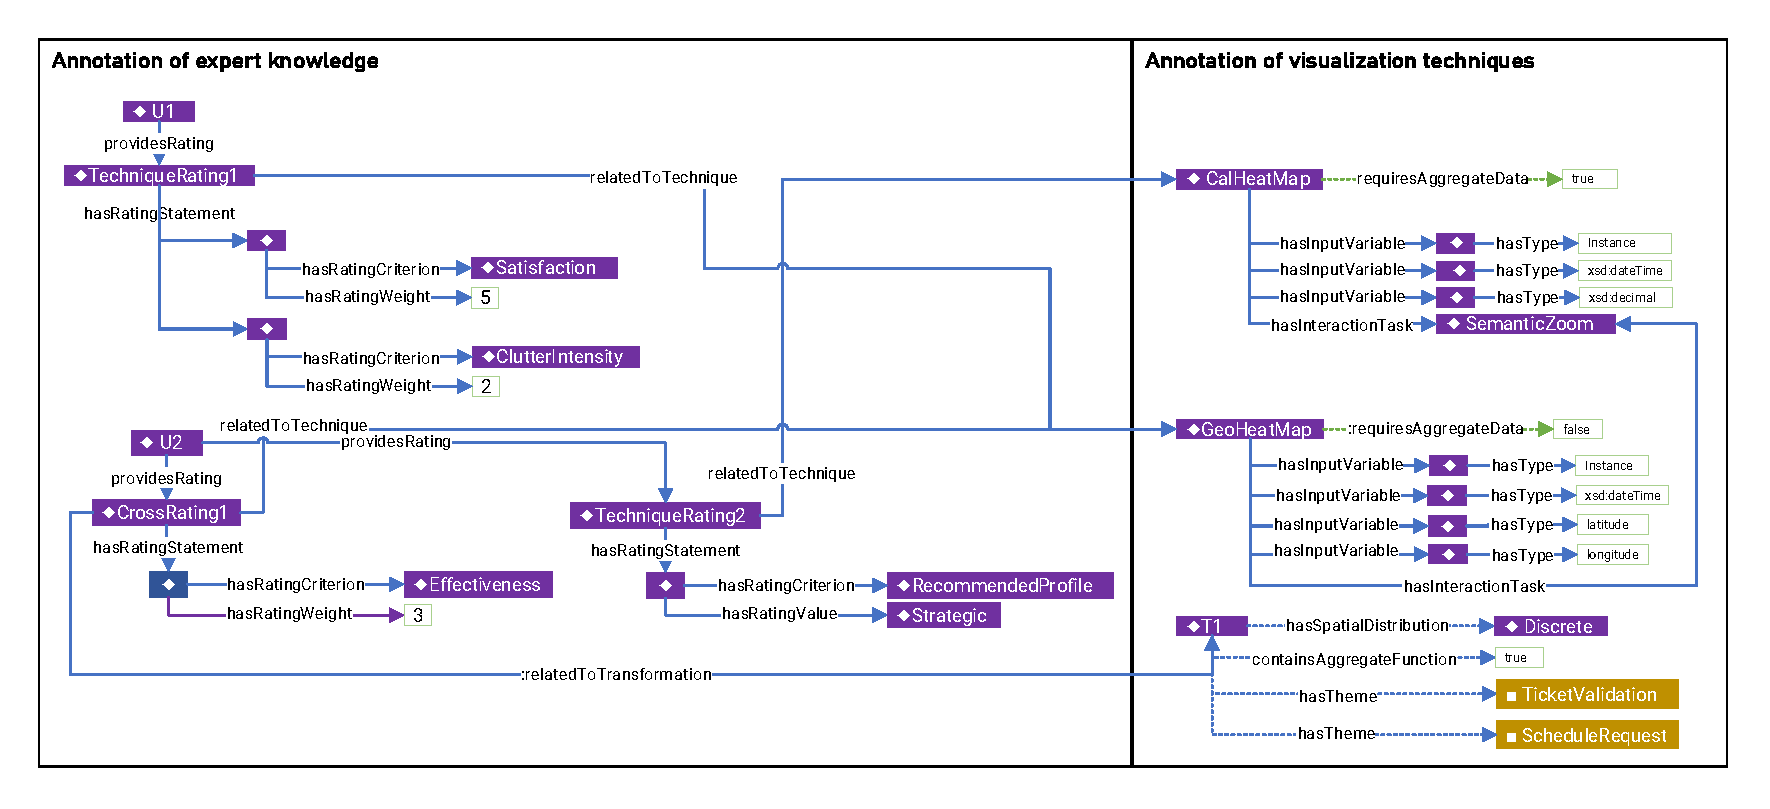
\includegraphics[width=\textwidth]{images/vis_user2.pdf}
\caption{Excerpt from RDF graph containing annotations about experts' knowledge (b) and visualization techniques (c).}
\label{fig:vis_user}
\end{sidewaysfigure}

\subsection{Expert Knowledge and Appropriateness Evaluation}

Let \textit{U1} and \textit{U2} be instances of \textit{DomainUser}, which represent two users of a visualization system, with strategic and operational profiles, respectively. \textit{Strategic} and \textit{Operational} are instances of \textit{DomainUserProfile}. Each user can rate a visualization technique with respect to multiple criteria represented by instances of \textit{RatingComponent}. Each criterion can be evaluated according to categorical or numerical values. Ratings are stored as instances of \textit{TechniqueRating}. Users can also provide a specialized rating that relates a visualization technique to a data transformation. Such rating is modeled as an instance of \textit{CrossRating}. Fig. \ref{fig:vis_user} exemplifies a general and specialized rating by \textit{U1} and \textit{U2}, respectively.

\textit{U1} stated that the \textit{GeoHeatMap} is appropriate for data transformations that induce a continuous domain. Quantitative ratings were also provided: \textit{Satisfaction} was rated "5" on an arbitrary scale of 0 to 5, and \textit{ClutterIntensity} was rated "2" on the same scale. The latter components are instances of \textit{Positive-} and \textit{NegativeRatingCriteria}, respectively. The type of each component can be used by a recommendation algorithm to define the appropriateness of each visualization technique.

\textit{U2} provided a specialized rating to the same technique and transformation \textit{T1}, and rated "3" on regards to the \textit{Effectiveness} criterion. The same user provided a global rating for \textit{GeoHeatMap}, in which it was stated that the technique is appropriate for users with a \textit{Strategic} profile.

%Appropriateness evaluation is specific to the urecommendation algorithm that should be implemented by a VRS. VUMO provides embedded functions (helpers) to assist methods on retrieving knowledge:
%
%\begin{itemize}
%    \item \textit{getTechniqueRating(t)}: returns all numeric ratings given to a visualization technique \textit{t};
%    \item \textit{getCrossRating(t,v)}: returns all cross ratings assigned to the visualization-transformation pair \textit{(t,v)};
%    \item \textit{getExpertInfo(e)}: returns asserted knowledged related to domain expert \textit{e}.
%\end{itemize}
%
%Helpers are also stored as SPARQL queries, and take advantage of the SPIN vocabulary to be executed as functions.

\subsection{Asserting new knowledge}

VUMO can be used to formalize new knowledge derived from the use of visualization techniques. In particular, the \textit{CalHeatmap} technique allowed the identification of an abnormal amount of schedule requests for Trindade, the main subway station in Porto. The number of requests is related to the public transportation strike that occurred on June 27th, 2013. The \textit{CalHeatMap} prototype was used to relate all schedule requrest instances on that date to a new event asserted as \textit{Strike27Jun13}, which is an instance of \textit{UnexpectedEvent}. Fig. \ref{fig:strike} shows the resulting graph.

\begin{figure}[!t]
\centering
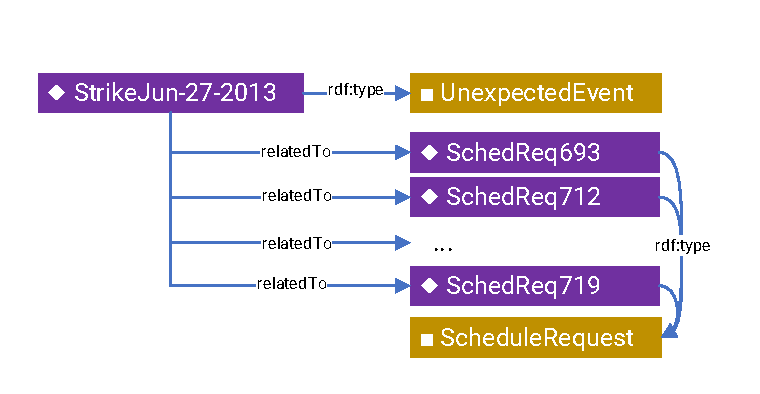
\includegraphics[width=9.3cm]{images/strike2.pdf}
\caption{An instance of \textit{UnexpectedEvent} represents a public transportation system strike, which is related to several \textit{ScheduleRequest}s}
\label{fig:strike}
\end{figure}


\section{Discussion of Results}
\label{sec:discussion}

For semantic integration of mobility data, the mapping of a dataset schema to VUMO classes and properties should be planned in advance. \textit{Ad hoc} parsers are considered an effective approach to convert raw data onto RDF graphs. A dataset may not be entirely described in terms of VUMO components due to the absence of specific classes or properties. To address that limitation, developers can extend or import additional ontologies which declare additional concepts.

The ontology does not require KVTs to be implemented in a specific programming language. To use VUMO, the only technological requirements are the support to RDF data, OWL ontologies and SPIN inference. Visualization techniques implemented in a VRS should be able to digest RDF data and comply to their annotation, especially on regards to the specification of input variables and interaction features.

KVTs may be impaired by cold start, i.e. absence or lack of sufficient domain expert knowledge to perform recommendations during early system use. VUMO addresses this limitation by evaluating compatibility (\textit{R5}), which can guarantee a minimal set of visualizations for experts to start with.

On regards to transformations, VUMO rules are limited to infer characteristics from queries, as the SPIN vocabulary allows them to be stored as a RDF graph. Still, transformations may assume other specialized forms, e.g. data mining algorithms or simulations. VUMO can still be useful to provide semantic annotation, as developers may manually specify such characteristics.


\section{Conclusion and Further Work}
\label{sec:conclusion}

This article proposed an ontology-based approach to integration and visualization of spatio-temporal urban mobility data from ITS. The core contribution is VUMO, an ontology that provides the semantic foundation for the development of Knowledge-assisted Visualization Systems. Such topic, to the best of our knowledge, has not yet been explored in Transportation studies.

The ontology provides two contributions; it specifies a formal vocabulary for describing spatial events in terms of the components of transportation networks, taking advantage of acknowledged ontologies for representing geospatial (GeoSPARQL, WGS84) and temporal (Time) data. The available constructs. Furthermore, visualization techniques can be described in terms of its features. Expert knowledge can be represented in terms of analytical profile of domain experts, ratings of visualization techniques, and analytical tasks consisting of one or more transformations.

A conceptual model, also introduced by this paper, was implemented into VUMO to derive visual features from such events, according to their semantic description. Such features are exploited by an expandable built-in ruleset to infer, for example, which visualizations are compatible and appropriate to represent a (sub)set of instance data.

A demonstration based on the city of Porto, Portugal, was introduced as a case study. It showed how multiple heterogeneous datasets could be semantically integrated. Prototypical visualization techniques and domain experts were defined to illustrate the implications of their characteristics on recommendation results.

As the ontology converges to its first stable version, an official specification and documentation will be disclosed, which will. Recently, the SPIN rule language has been standardized into SHACL (Shapes Constraint Language) by the W3C; the language is considered to be an evolution of OWL. We plan to translate VUMO into SHACL, so that researchers and practitioners can opt for OWL or SHACL, in accordance to their requirements. Nonetheless, we alert the reader that, by the time of this thesis, few Semantic Web based systems fully support SHACL. We also plan to provide an online shared repository for reuse of empirical knowledge. This would allow researchers and practitioners from various contexts to reuse knowledge made public from other studies or actual practical contexts. This idea is aligned with our orientation towards the involvement of domain experts throughout the visualization process. Moreover, the idea is also aligned with the Semantic Web principle of reusing existing knowledge, to enhance the capability of other systems that also make use of such technologies.

\section*{Acknowledgements}

 We thank Transportes Intermodais do Porto (TIP) and Optimiza\c{c}\~{a}o e Planeamento de Transportes S.A. (OPT) for providing the datasets.



\section*{Funding}

This work was funded by Funda\c{c}\~{a}o para Ci\^{e}ncia e Tecnologia (FCT), grant number PD/BD/105910/2014, by the ERDF - European Regional Development Fund through the Operational Programme for Competitiveness and Internationalisation - COMPETE 2020 Programme, and by National Funds through the Portuguese funding agency, FCT - Fundação para a Ciência e a Tecnologia within project POCI-01-0145-FEDER-032053 / PTDC/ECI-TRA/32053/2017.


\bibliographystyle{apacite}
\bibliography{library}



\end{document}
